% Options for packages loaded elsewhere
% Options for packages loaded elsewhere
\PassOptionsToPackage{unicode}{hyperref}
\PassOptionsToPackage{hyphens}{url}
\PassOptionsToPackage{dvipsnames,svgnames,x11names}{xcolor}
%
\documentclass[
  spanish,
  letterpaper,
]{scrbook}
\usepackage{xcolor}
\usepackage[top=2.4cm,bottom=2.4cm,left=2.6cm,right=2.4cm]{geometry}
\usepackage{amsmath,amssymb}
\setcounter{secnumdepth}{5}
\usepackage{iftex}
\ifPDFTeX
  \usepackage[T1]{fontenc}
  \usepackage[utf8]{inputenc}
  \usepackage{textcomp} % provide euro and other symbols
\else % if luatex or xetex
  \usepackage{unicode-math} % this also loads fontspec
  \defaultfontfeatures{Scale=MatchLowercase}
  \defaultfontfeatures[\rmfamily]{Ligatures=TeX,Scale=1}
\fi
\usepackage{lmodern}
\ifPDFTeX\else
  % xetex/luatex font selection
  \setmainfont[]{Arial}
  \setmonofont[]{Courier New}
\fi
% Use upquote if available, for straight quotes in verbatim environments
\IfFileExists{upquote.sty}{\usepackage{upquote}}{}
\IfFileExists{microtype.sty}{% use microtype if available
  \usepackage[]{microtype}
  \UseMicrotypeSet[protrusion]{basicmath} % disable protrusion for tt fonts
}{}
\makeatletter
\@ifundefined{KOMAClassName}{% if non-KOMA class
  \IfFileExists{parskip.sty}{%
    \usepackage{parskip}
  }{% else
    \setlength{\parindent}{0pt}
    \setlength{\parskip}{6pt plus 2pt minus 1pt}}
}{% if KOMA class
  \KOMAoptions{parskip=half}}
\makeatother
% Make \paragraph and \subparagraph free-standing
\makeatletter
\ifx\paragraph\undefined\else
  \let\oldparagraph\paragraph
  \renewcommand{\paragraph}{
    \@ifstar
      \xxxParagraphStar
      \xxxParagraphNoStar
  }
  \newcommand{\xxxParagraphStar}[1]{\oldparagraph*{#1}\mbox{}}
  \newcommand{\xxxParagraphNoStar}[1]{\oldparagraph{#1}\mbox{}}
\fi
\ifx\subparagraph\undefined\else
  \let\oldsubparagraph\subparagraph
  \renewcommand{\subparagraph}{
    \@ifstar
      \xxxSubParagraphStar
      \xxxSubParagraphNoStar
  }
  \newcommand{\xxxSubParagraphStar}[1]{\oldsubparagraph*{#1}\mbox{}}
  \newcommand{\xxxSubParagraphNoStar}[1]{\oldsubparagraph{#1}\mbox{}}
\fi
\makeatother

\usepackage{color}
\usepackage{fancyvrb}
\newcommand{\VerbBar}{|}
\newcommand{\VERB}{\Verb[commandchars=\\\{\}]}
\DefineVerbatimEnvironment{Highlighting}{Verbatim}{commandchars=\\\{\}}
% Add ',fontsize=\small' for more characters per line
\usepackage{framed}
\definecolor{shadecolor}{RGB}{241,243,245}
\newenvironment{Shaded}{\begin{snugshade}}{\end{snugshade}}
\newcommand{\AlertTok}[1]{\textcolor[rgb]{0.68,0.00,0.00}{#1}}
\newcommand{\AnnotationTok}[1]{\textcolor[rgb]{0.37,0.37,0.37}{#1}}
\newcommand{\AttributeTok}[1]{\textcolor[rgb]{0.40,0.45,0.13}{#1}}
\newcommand{\BaseNTok}[1]{\textcolor[rgb]{0.68,0.00,0.00}{#1}}
\newcommand{\BuiltInTok}[1]{\textcolor[rgb]{0.00,0.23,0.31}{#1}}
\newcommand{\CharTok}[1]{\textcolor[rgb]{0.13,0.47,0.30}{#1}}
\newcommand{\CommentTok}[1]{\textcolor[rgb]{0.37,0.37,0.37}{#1}}
\newcommand{\CommentVarTok}[1]{\textcolor[rgb]{0.37,0.37,0.37}{\textit{#1}}}
\newcommand{\ConstantTok}[1]{\textcolor[rgb]{0.56,0.35,0.01}{#1}}
\newcommand{\ControlFlowTok}[1]{\textcolor[rgb]{0.00,0.23,0.31}{\textbf{#1}}}
\newcommand{\DataTypeTok}[1]{\textcolor[rgb]{0.68,0.00,0.00}{#1}}
\newcommand{\DecValTok}[1]{\textcolor[rgb]{0.68,0.00,0.00}{#1}}
\newcommand{\DocumentationTok}[1]{\textcolor[rgb]{0.37,0.37,0.37}{\textit{#1}}}
\newcommand{\ErrorTok}[1]{\textcolor[rgb]{0.68,0.00,0.00}{#1}}
\newcommand{\ExtensionTok}[1]{\textcolor[rgb]{0.00,0.23,0.31}{#1}}
\newcommand{\FloatTok}[1]{\textcolor[rgb]{0.68,0.00,0.00}{#1}}
\newcommand{\FunctionTok}[1]{\textcolor[rgb]{0.28,0.35,0.67}{#1}}
\newcommand{\ImportTok}[1]{\textcolor[rgb]{0.00,0.46,0.62}{#1}}
\newcommand{\InformationTok}[1]{\textcolor[rgb]{0.37,0.37,0.37}{#1}}
\newcommand{\KeywordTok}[1]{\textcolor[rgb]{0.00,0.23,0.31}{\textbf{#1}}}
\newcommand{\NormalTok}[1]{\textcolor[rgb]{0.00,0.23,0.31}{#1}}
\newcommand{\OperatorTok}[1]{\textcolor[rgb]{0.37,0.37,0.37}{#1}}
\newcommand{\OtherTok}[1]{\textcolor[rgb]{0.00,0.23,0.31}{#1}}
\newcommand{\PreprocessorTok}[1]{\textcolor[rgb]{0.68,0.00,0.00}{#1}}
\newcommand{\RegionMarkerTok}[1]{\textcolor[rgb]{0.00,0.23,0.31}{#1}}
\newcommand{\SpecialCharTok}[1]{\textcolor[rgb]{0.37,0.37,0.37}{#1}}
\newcommand{\SpecialStringTok}[1]{\textcolor[rgb]{0.13,0.47,0.30}{#1}}
\newcommand{\StringTok}[1]{\textcolor[rgb]{0.13,0.47,0.30}{#1}}
\newcommand{\VariableTok}[1]{\textcolor[rgb]{0.07,0.07,0.07}{#1}}
\newcommand{\VerbatimStringTok}[1]{\textcolor[rgb]{0.13,0.47,0.30}{#1}}
\newcommand{\WarningTok}[1]{\textcolor[rgb]{0.37,0.37,0.37}{\textit{#1}}}

\usepackage{longtable,booktabs,array}
\newcounter{none} % for unnumbered tables
\usepackage{calc} % for calculating minipage widths
% Correct order of tables after \paragraph or \subparagraph
\usepackage{etoolbox}
\makeatletter
\patchcmd\longtable{\par}{\if@noskipsec\mbox{}\fi\par}{}{}
\makeatother
% Allow footnotes in longtable head/foot
\IfFileExists{footnotehyper.sty}{\usepackage{footnotehyper}}{\usepackage{footnote}}
\makesavenoteenv{longtable}
\usepackage{graphicx}
\makeatletter
\newsavebox\pandoc@box
\newcommand*\pandocbounded[1]{% scales image to fit in text height/width
  \sbox\pandoc@box{#1}%
  \Gscale@div\@tempa{\textheight}{\dimexpr\ht\pandoc@box+\dp\pandoc@box\relax}%
  \Gscale@div\@tempb{\linewidth}{\wd\pandoc@box}%
  \ifdim\@tempb\p@<\@tempa\p@\let\@tempa\@tempb\fi% select the smaller of both
  \ifdim\@tempa\p@<\p@\scalebox{\@tempa}{\usebox\pandoc@box}%
  \else\usebox{\pandoc@box}%
  \fi%
}
% Set default figure placement to htbp
\def\fps@figure{htbp}
\makeatother



\ifLuaTeX
\usepackage[bidi=basic,shorthands=off]{babel}
\else
\usepackage[bidi=default,shorthands=off]{babel}
\fi
\ifPDFTeX
\else
\babelfont{rm}[]{Arial}
\fi
\ifLuaTeX
  \usepackage{selnolig} % disable illegal ligatures
\fi


\setlength{\emergencystretch}{3em} % prevent overfull lines

\providecommand{\tightlist}{%
  \setlength{\itemsep}{0pt}\setlength{\parskip}{0pt}}



 


\usepackage{fancyhdr}
\usepackage{xcolor}
\usepackage{titlesec}
\usepackage{graphicx}
\usepackage{longtable}
\usepackage{booktabs}
\definecolor{umgblue}{HTML}{1F4E79}
\definecolor{umggray}{HTML}{646464}
\definecolor{umglight}{HTML}{EEF1F4}
\pagestyle{fancy}
\fancyhf{}
\lhead{\textcolor{umggray}{Editorial Académica}}
\rhead{\textcolor{umggray}{Ingeniería en Sistemas}}
\cfoot{\textcolor{umggray}{\thepage}}
\renewcommand{\headrulewidth}{0.3pt}
\renewcommand{\headrule}{\hbox to\headwidth{\color{umgblue}\leaders\hrule height \headrulewidth\hfill}}
\titleformat{\chapter}{\Huge\bfseries\color{umgblue}}{\thechapter}{1em}{}
\titleformat{\section}{\Large\bfseries\color{umgblue}}{\thesection}{1em}{}
\titleformat{\subsection}{\large\bfseries\color{umggray}}{\thesubsection}{1em}{}
\makeatletter
\@ifpackageloaded{tcolorbox}{}{\usepackage[skins,breakable]{tcolorbox}}
\@ifpackageloaded{fontawesome5}{}{\usepackage{fontawesome5}}
\definecolor{quarto-callout-color}{HTML}{909090}
\definecolor{quarto-callout-note-color}{HTML}{0758E5}
\definecolor{quarto-callout-important-color}{HTML}{CC1914}
\definecolor{quarto-callout-warning-color}{HTML}{EB9113}
\definecolor{quarto-callout-tip-color}{HTML}{00A047}
\definecolor{quarto-callout-caution-color}{HTML}{FC5300}
\definecolor{quarto-callout-color-frame}{HTML}{acacac}
\definecolor{quarto-callout-note-color-frame}{HTML}{4582ec}
\definecolor{quarto-callout-important-color-frame}{HTML}{d9534f}
\definecolor{quarto-callout-warning-color-frame}{HTML}{f0ad4e}
\definecolor{quarto-callout-tip-color-frame}{HTML}{02b875}
\definecolor{quarto-callout-caution-color-frame}{HTML}{fd7e14}
\makeatother
\makeatletter
\@ifpackageloaded{bookmark}{}{\usepackage{bookmark}}
\makeatother
\makeatletter
\@ifpackageloaded{caption}{}{\usepackage{caption}}
\AtBeginDocument{%
\ifdefined\contentsname
  \renewcommand*\contentsname{Tabla de contenidos}
\else
  \newcommand\contentsname{Tabla de contenidos}
\fi
\ifdefined\listfigurename
  \renewcommand*\listfigurename{Listado de Figuras}
\else
  \newcommand\listfigurename{Listado de Figuras}
\fi
\ifdefined\listtablename
  \renewcommand*\listtablename{Listado de Tablas}
\else
  \newcommand\listtablename{Listado de Tablas}
\fi
\ifdefined\figurename
  \renewcommand*\figurename{Figura}
\else
  \newcommand\figurename{Figura}
\fi
\ifdefined\tablename
  \renewcommand*\tablename{Tabla}
\else
  \newcommand\tablename{Tabla}
\fi
}
\@ifpackageloaded{float}{}{\usepackage{float}}
\floatstyle{ruled}
\@ifundefined{c@chapter}{\newfloat{codelisting}{h}{lop}}{\newfloat{codelisting}{h}{lop}[chapter]}
\floatname{codelisting}{Listado}
\newcommand*\listoflistings{\listof{codelisting}{Listado de Listados}}
\makeatother
\makeatletter
\makeatother
\makeatletter
\@ifpackageloaded{caption}{}{\usepackage{caption}}
\@ifpackageloaded{subcaption}{}{\usepackage{subcaption}}
\makeatother
\usepackage{bookmark}
\IfFileExists{xurl.sty}{\usepackage{xurl}}{} % add URL line breaks if available
\urlstyle{same}
\hypersetup{
  pdftitle={Portada},
  pdflang={es},
  colorlinks=true,
  linkcolor={Maroon},
  filecolor={Maroon},
  citecolor={Blue},
  urlcolor={Blue},
  pdfcreator={LaTeX via pandoc}}


\title{Portada}
\author{}
\date{}
\begin{document}
\frontmatter
\maketitle

\renewcommand*\contentsname{Contenido}
{
\setcounter{tocdepth}{2}
\tableofcontents
}

\mainmatter
\bookmarksetup{startatroot}

\chapter{Portada}\label{portada}

\begin{titlepage}
\centering
\vspace*{1.5cm}
{\Large UNIVERSIDAD MARIANO GÁLVEZ DE GUATEMALA\par}
\vspace{0.4cm}
{\large Facultad de Ingeniería en Sistemas\par}
\vspace{1.5cm}
{\Huge\bfseries SISTEMAS OPERATIVOS I\par}
\vspace{0.5cm}
{\Large Introducción y fundamentos\par}
\vspace{1.2cm}
{\LARGE Clase 1\par}
\vspace{0.3cm}
{\Large Introducción a los Sistemas Operativos\par}
\vfill
{\Large Ing. Jorge Luis García Chacón\par}
\vspace{0.5cm}
{\large Segundo Semestre - Edición 2026\par}
\vspace{1.2cm}
{\itshape El libro que nos hubiera gustado tener cuando estudiábamos Ingeniería.\par}
\end{titlepage}
\clearpage

\bookmarksetup{startatroot}

\chapter{Acerca de este volumen}\label{acerca-de-este-volumen}

{\def\LTcaptype{none} % do not increment counter
\begin{longtable}[]{@{}ll@{}}
\toprule\noalign{}
Campo & Información \\
\midrule\noalign{}
\endhead
\bottomrule\noalign{}
\endlastfoot
Universidad & Universidad Mariano Gálvez de Guatemala \\
Facultad & Ingeniería en Sistemas \\
Colección & Editorial Académica de Ingeniería en Sistemas \\
Curso & Sistemas Operativos I \\
Clase & Introducción a los Sistemas Operativos \\
Docente & Ing. Jorge Luis García Chacón \\
Edición & 2026 \\
\end{longtable}
}

\begin{tcolorbox}[enhanced jigsaw, arc=.35mm, bottomrule=.15mm, bottomtitle=1mm, breakable, colback=white, colbacktitle=quarto-callout-note-color!10!white, colframe=quarto-callout-note-color-frame, coltitle=black, left=2mm, leftrule=.75mm, opacityback=0, opacitybacktitle=0.6, rightrule=.15mm, title=\textcolor{quarto-callout-note-color}{\faInfo}\hspace{0.5em}{Propósito de la colección}, titlerule=0mm, toprule=.15mm, toptitle=1mm]

Esta colección transforma la experiencia docente en materiales
universitarios claros, actuales, prácticos y reutilizables.

\end{tcolorbox}

\begin{tcolorbox}[enhanced jigsaw, arc=.35mm, bottomrule=.15mm, bottomtitle=1mm, breakable, colback=white, colbacktitle=quarto-callout-tip-color!10!white, colframe=quarto-callout-tip-color-frame, coltitle=black, left=2mm, leftrule=.75mm, opacityback=0, opacitybacktitle=0.6, rightrule=.15mm, title=\textcolor{quarto-callout-tip-color}{\faLightbulb}\hspace{0.5em}{Lema editorial}, titlerule=0mm, toprule=.15mm, toptitle=1mm]

Diseñar una vez. Enseñar toda la vida.

\end{tcolorbox}

\bookmarksetup{startatroot}

\chapter{Presentación de la clase}\label{presentaciuxf3n-de-la-clase}

Bienvenidos al curso de \textbf{Sistemas Operativos I}. En esta primera
clase estudiaremos el software que coordina prácticamente todo lo que
ocurre en una computadora, un teléfono, un servidor o un dispositivo
inteligente.

Imagine que enciende su computadora y, en pocos segundos, puede abrir un
navegador, reproducir música, guardar archivos, conectarse a Internet y
utilizar varios programas al mismo tiempo. Mientras usted observa una
pantalla aparentemente sencilla, el equipo está detectando dispositivos,
reservando memoria, iniciando servicios, creando procesos, aplicando
controles de seguridad y organizando el acceso al almacenamiento.

La pieza que coordina esas actividades es el \textbf{sistema operativo}.

\begin{tcolorbox}[enhanced jigsaw, arc=.35mm, bottomrule=.15mm, bottomtitle=1mm, breakable, colback=white, colbacktitle=quarto-callout-note-color!10!white, colframe=quarto-callout-note-color-frame, coltitle=black, left=2mm, leftrule=.75mm, opacityback=0, opacitybacktitle=0.6, rightrule=.15mm, title=\textcolor{quarto-callout-note-color}{\faInfo}\hspace{0.5em}{Idea central de la clase}, titlerule=0mm, toprule=.15mm, toptitle=1mm]

El sistema operativo administra recursos, ofrece servicios a los
programas y crea un entorno seguro y utilizable para las personas y las
aplicaciones.

\end{tcolorbox}

\section{Objetivos de aprendizaje}\label{objetivos-de-aprendizaje}

Al finalizar esta clase, el estudiante será capaz de:

\begin{itemize}
\tightlist
\item
  Explicar qué es un sistema operativo y por qué es indispensable.
\item
  Identificar la relación entre usuario, aplicaciones, sistema operativo
  y hardware.
\item
  Reconocer las funciones principales del sistema operativo.
\item
  Diferenciar una interfaz gráfica de una interfaz de línea de comandos.
\item
  Clasificar sistemas operativos según su propósito y forma de trabajo.
\item
  Explicar, de manera introductoria, qué son el kernel, los procesos y
  las llamadas al sistema.
\item
  Identificar el sistema operativo, la versión y las características
  básicas de su propio equipo.
\end{itemize}

\begin{tcolorbox}[enhanced jigsaw, arc=.35mm, bottomrule=.15mm, bottomtitle=1mm, breakable, colback=white, colbacktitle=quarto-callout-tip-color!10!white, colframe=quarto-callout-tip-color-frame, coltitle=black, left=2mm, leftrule=.75mm, opacityback=0, opacitybacktitle=0.6, rightrule=.15mm, title=\textcolor{quarto-callout-tip-color}{\faLightbulb}\hspace{0.5em}{El libro que nos hubiera gustado tener}, titlerule=0mm, toprule=.15mm, toptitle=1mm]

En este curso no memorizaremos listas aisladas. Relacionaremos cada
concepto con situaciones que un ingeniero encontrará al administrar
computadoras, servidores, redes y aplicaciones.

\end{tcolorbox}

\bookmarksetup{startatroot}

\chapter{¿Qué es un sistema
operativo?}\label{quuxe9-es-un-sistema-operativo}

Un \textbf{sistema operativo} es el software fundamental que administra
los recursos de un sistema informático y proporciona servicios comunes
para que las aplicaciones puedan ejecutarse.

Actúa como intermediario entre:

\begin{itemize}
\tightlist
\item
  las personas que utilizan el equipo;
\item
  las aplicaciones;
\item
  el hardware;
\item
  y los dispositivos conectados.
\end{itemize}

Sin un sistema operativo, cada programa tendría que conocer directamente
cómo funciona cada modelo de procesador, disco, teclado, tarjeta de red
o pantalla. El sistema operativo reduce esa complejidad mediante
servicios y abstracciones.

\begin{figure}[H]

{\centering 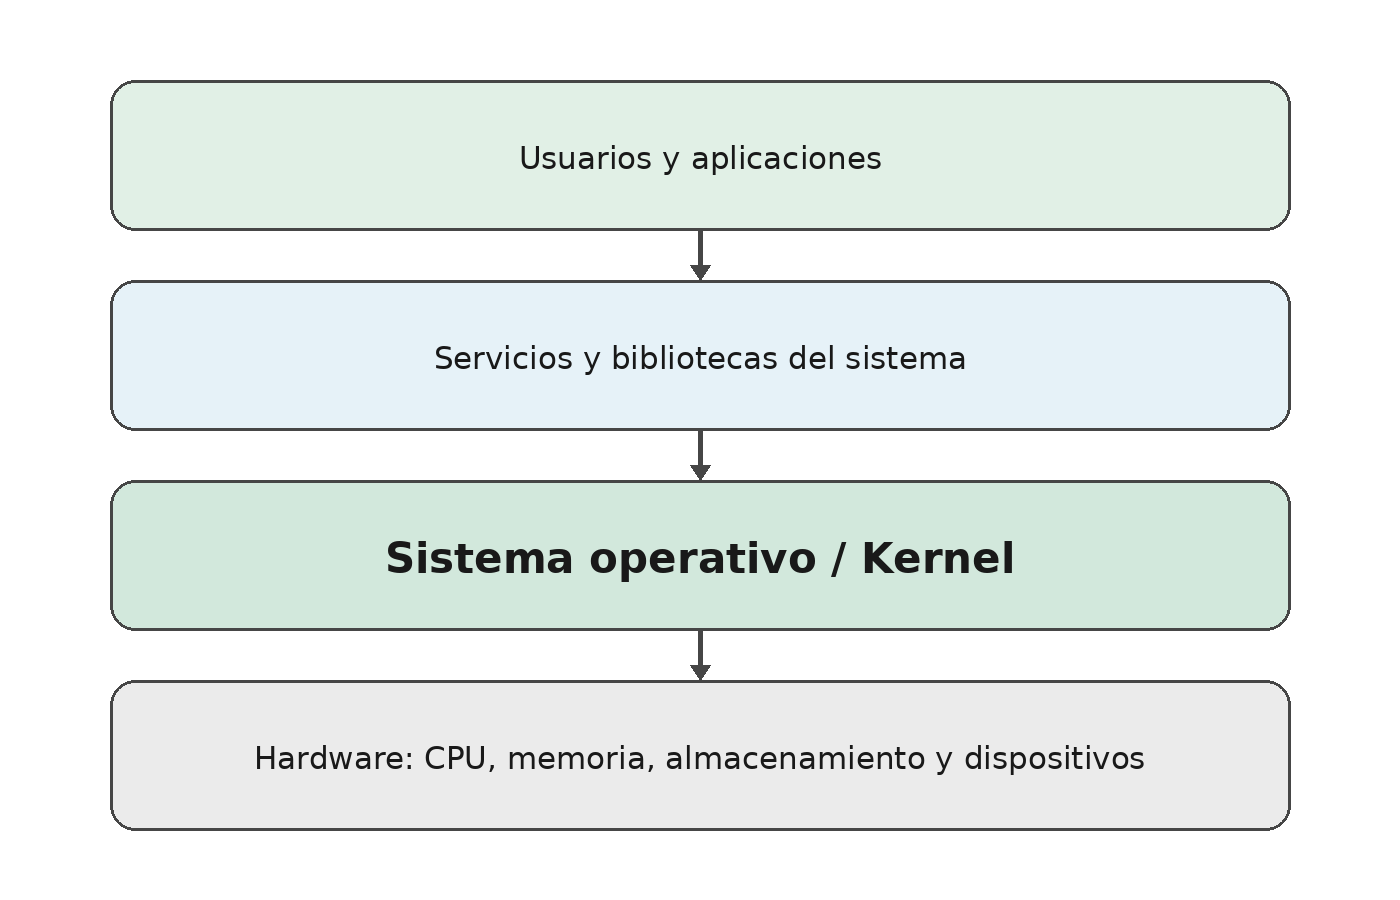
\includegraphics[width=0.88\linewidth,height=\textheight,keepaspectratio]{capitulos/../assets/img/capas_sistema_operativo.png}

}

\caption{Capas principales de un sistema informático}

\end{figure}%

\section{Una comparación sencilla}\label{una-comparaciuxf3n-sencilla}

Pensemos en un hotel:

\begin{itemize}
\tightlist
\item
  Los \textbf{huéspedes} representan a los usuarios y aplicaciones.
\item
  Las \textbf{habitaciones, energía, ascensores y servicios} representan
  los recursos de hardware.
\item
  La \textbf{administración del hotel} representa al sistema operativo.
\end{itemize}

Cada huésped utiliza servicios sin controlar directamente toda la
infraestructura. La administración asigna recursos, organiza
prioridades, establece reglas y evita conflictos.

\begin{tcolorbox}[enhanced jigsaw, arc=.35mm, bottomrule=.15mm, bottomtitle=1mm, breakable, colback=white, colbacktitle=quarto-callout-important-color!10!white, colframe=quarto-callout-important-color-frame, coltitle=black, left=2mm, leftrule=.75mm, opacityback=0, opacitybacktitle=0.6, rightrule=.15mm, title=\textcolor{quarto-callout-important-color}{\faExclamation}\hspace{0.5em}{Importante}, titlerule=0mm, toprule=.15mm, toptitle=1mm]

El sistema operativo no es únicamente la apariencia del escritorio. La
interfaz gráfica es solo una de sus capas. Debajo de ella existen
procesos, controladores, servicios, mecanismos de seguridad y un kernel
que trabaja continuamente.

\end{tcolorbox}

\bookmarksetup{startatroot}

\chapter{El kernel: núcleo del sistema
operativo}\label{el-kernel-nuxfacleo-del-sistema-operativo}

El \textbf{kernel} es la parte central del sistema operativo. Se ejecuta
con privilegios elevados y controla el acceso a los recursos esenciales
del computador.

Entre sus responsabilidades se encuentran:

\begin{itemize}
\tightlist
\item
  planificar el uso del procesador;
\item
  administrar la memoria;
\item
  controlar dispositivos mediante controladores;
\item
  coordinar operaciones de entrada y salida;
\item
  aplicar mecanismos de protección;
\item
  ofrecer servicios a los programas mediante llamadas al sistema.
\end{itemize}

El kernel no debe confundirse con todo el sistema operativo. Un sistema
completo también incluye bibliotecas, utilidades, servicios,
herramientas administrativas e interfaces de usuario.

\section{Modo usuario y modo
privilegiado}\label{modo-usuario-y-modo-privilegiado}

Los procesadores modernos permiten separar al menos dos niveles de
ejecución:

{\def\LTcaptype{none} % do not increment counter
\begin{longtable}[]{@{}
  >{\raggedright\arraybackslash}p{(\linewidth - 4\tabcolsep) * \real{0.3333}}
  >{\raggedright\arraybackslash}p{(\linewidth - 4\tabcolsep) * \real{0.3333}}
  >{\raggedright\arraybackslash}p{(\linewidth - 4\tabcolsep) * \real{0.3333}}@{}}
\toprule\noalign{}
\begin{minipage}[b]{\linewidth}\raggedright
Nivel
\end{minipage} & \begin{minipage}[b]{\linewidth}\raggedright
Característica principal
\end{minipage} & \begin{minipage}[b]{\linewidth}\raggedright
Ejemplo
\end{minipage} \\
\midrule\noalign{}
\endhead
\bottomrule\noalign{}
\endlastfoot
Modo usuario & Acceso limitado; las aplicaciones no controlan
directamente todo el hardware & Navegador, editor de texto,
reproductor \\
Modo kernel o privilegiado & Acceso a operaciones críticas y recursos
protegidos & Kernel, controladores y componentes esenciales \\
\end{longtable}
}

Esta separación evita que un error común en una aplicación tenga acceso
irrestricto a toda la memoria o a los dispositivos del sistema.

\begin{tcolorbox}[enhanced jigsaw, arc=.35mm, bottomrule=.15mm, bottomtitle=1mm, breakable, colback=white, colbacktitle=quarto-callout-warning-color!10!white, colframe=quarto-callout-warning-color-frame, coltitle=black, left=2mm, leftrule=.75mm, opacityback=0, opacitybacktitle=0.6, rightrule=.15mm, title=\textcolor{quarto-callout-warning-color}{\faExclamationTriangle}\hspace{0.5em}{Error común}, titlerule=0mm, toprule=.15mm, toptitle=1mm]

Decir que una aplicación ``habla directamente con el hardware'' suele
ser una simplificación. En la mayoría de los casos, la aplicación
solicita servicios al sistema operativo, y este coordina la operación
con el hardware.

\end{tcolorbox}

\bookmarksetup{startatroot}

\chapter{Funciones principales de un sistema
operativo}\label{funciones-principales-de-un-sistema-operativo}

\section{Gestión de procesos}\label{gestiuxf3n-de-procesos}

Un \textbf{proceso} es un programa en ejecución. El sistema operativo
debe decidir:

\begin{itemize}
\tightlist
\item
  qué proceso utiliza el procesador;
\item
  durante cuánto tiempo;
\item
  cuándo se pausa;
\item
  cuándo continúa;
\item
  y cómo se comunica con otros procesos.
\end{itemize}

Cuando una persona abre un navegador, un editor y una videollamada, el
equipo parece ejecutar todo simultáneamente. En realidad, el sistema
operativo distribuye el tiempo del procesador entre muchas actividades,
aprovechando además los múltiples núcleos de la CPU.

\section{Gestión de memoria}\label{gestiuxf3n-de-memoria}

El sistema operativo asigna memoria a cada proceso y procura que una
aplicación no modifique sin autorización la memoria de otra.

También puede utilizar \textbf{memoria virtual}, una técnica que permite
organizar el espacio de direcciones de los procesos y, cuando es
necesario, apoyar temporalmente la memoria física con almacenamiento
secundario.

\section{Gestión de archivos y
almacenamiento}\label{gestiuxf3n-de-archivos-y-almacenamiento}

El sistema operativo organiza la información mediante archivos,
carpetas, permisos y sistemas de archivos.

Entre sus tareas se encuentran:

\begin{itemize}
\tightlist
\item
  crear, leer, modificar y eliminar archivos;
\item
  organizar directorios;
\item
  controlar permisos;
\item
  registrar ubicaciones y metadatos;
\item
  coordinar el uso de discos, memorias USB y otras unidades.
\end{itemize}

\section{Gestión de dispositivos}\label{gestiuxf3n-de-dispositivos}

Los dispositivos poseen características distintas. Para utilizarlos, el
sistema operativo emplea \textbf{controladores} o \emph{drivers}.

Un controlador traduce solicitudes generales del sistema a operaciones
específicas del dispositivo. Gracias a esta capa, una aplicación puede
imprimir sin conocer todos los detalles internos de cada impresora.

\section{Seguridad y protección}\label{seguridad-y-protecciuxf3n}

El sistema operativo administra usuarios, sesiones, permisos,
credenciales y aislamiento entre procesos.

La seguridad no consiste únicamente en utilizar una contraseña. También
incluye:

\begin{itemize}
\tightlist
\item
  controlar quién puede acceder a un archivo;
\item
  limitar privilegios;
\item
  proteger la memoria;
\item
  aplicar actualizaciones;
\item
  registrar eventos;
\item
  bloquear operaciones no autorizadas.
\end{itemize}

\section{Redes y comunicación}\label{redes-y-comunicaciuxf3n}

Los sistemas operativos modernos incluyen una pila de red que permite
utilizar protocolos, interfaces, puertos y servicios de comunicación.

Cuando un navegador accede a una página web, el sistema operativo
participa en la resolución de nombres, el envío de paquetes, la
recepción de información y la entrega de datos a la aplicación
correspondiente.

\begin{tcolorbox}[enhanced jigsaw, arc=.35mm, bottomrule=.15mm, bottomtitle=1mm, breakable, colback=white, colbacktitle=quarto-callout-tip-color!10!white, colframe=quarto-callout-tip-color-frame, coltitle=black, left=2mm, leftrule=.75mm, opacityback=0, opacitybacktitle=0.6, rightrule=.15mm, title=\textcolor{quarto-callout-tip-color}{\faLightbulb}\hspace{0.5em}{En la práctica profesional}, titlerule=0mm, toprule=.15mm, toptitle=1mm]

Cuando un servidor deja de responder, un administrador no debería
comenzar reinstalando el sistema operativo. Primero revisa el uso de
CPU, memoria, disco, red, procesos y registros para identificar la causa
del problema.

\end{tcolorbox}

\bookmarksetup{startatroot}

\chapter{Breve evolución de los sistemas
operativos}\label{breve-evoluciuxf3n-de-los-sistemas-operativos}

La evolución de los sistemas operativos está estrechamente relacionada
con la evolución del hardware y las necesidades de los usuarios.

\section{Primeras computadoras}\label{primeras-computadoras}

En las primeras generaciones, los programas se cargaban manualmente y el
operador controlaba gran parte del proceso. El tiempo de la computadora
era costoso y se perdía mucho tiempo preparando cada trabajo.

\section{Monitor residente}\label{monitor-residente}

El \textbf{monitor residente} permanecía en memoria y automatizaba parte
de la carga y ejecución de programas. Fue un paso inicial hacia la
coordinación automática de trabajos.

\section{Procesamiento por lotes}\label{procesamiento-por-lotes}

El procesamiento por lotes agrupó varios trabajos para ejecutarlos
secuencialmente con poca interacción humana. Esta modalidad mejoró la
utilización del equipo, aunque el usuario debía esperar para recibir
resultados.

\section{Multiprogramación y tiempo
compartido}\label{multiprogramaciuxf3n-y-tiempo-compartido}

La multiprogramación permitió mantener varios trabajos en memoria y
utilizar el procesador mientras otro esperaba una operación de entrada o
salida.

El tiempo compartido extendió esta idea para atender a varios usuarios
de forma interactiva, ofreciendo la impresión de que cada uno disponía
del sistema.

\section{Computadoras personales e interfaces
gráficas}\label{computadoras-personales-e-interfaces-gruxe1ficas}

Las computadoras personales acercaron la informática a hogares y
oficinas. Las interfaces gráficas facilitaron el uso mediante ventanas,
iconos, menús y dispositivos apuntadores.

\section{Internet, dispositivos móviles, nube y
virtualización}\label{internet-dispositivos-muxf3viles-nube-y-virtualizaciuxf3n}

Los sistemas actuales ya no se limitan a una computadora de escritorio.
Existen sistemas para:

\begin{itemize}
\tightlist
\item
  servidores físicos y virtuales;
\item
  teléfonos y tabletas;
\item
  dispositivos integrados;
\item
  infraestructura en la nube;
\item
  vehículos y equipos industriales;
\item
  plataformas de contenedores.
\end{itemize}

\begin{tcolorbox}[enhanced jigsaw, arc=.35mm, bottomrule=.15mm, bottomtitle=1mm, breakable, colback=white, colbacktitle=quarto-callout-note-color!10!white, colframe=quarto-callout-note-color-frame, coltitle=black, left=2mm, leftrule=.75mm, opacityback=0, opacitybacktitle=0.6, rightrule=.15mm, title=\textcolor{quarto-callout-note-color}{\faInfo}\hspace{0.5em}{Perspectiva histórica}, titlerule=0mm, toprule=.15mm, toptitle=1mm]

Los sistemas antiguos como MS-DOS, Windows XP o las primeras versiones
de Mac OS siguen siendo importantes para comprender la evolución, pero
no deben presentarse como el panorama tecnológico actual.

\end{tcolorbox}

\bookmarksetup{startatroot}

\chapter{Panorama actual de sistemas
operativos}\label{panorama-actual-de-sistemas-operativos}

La siguiente tabla presenta familias relevantes para un estudiante de
Ingeniería en Sistemas.

{\def\LTcaptype{none} % do not increment counter
\begin{longtable}[]{@{}
  >{\raggedright\arraybackslash}p{(\linewidth - 4\tabcolsep) * \real{0.3333}}
  >{\raggedright\arraybackslash}p{(\linewidth - 4\tabcolsep) * \real{0.3333}}
  >{\raggedright\arraybackslash}p{(\linewidth - 4\tabcolsep) * \real{0.3333}}@{}}
\toprule\noalign{}
\begin{minipage}[b]{\linewidth}\raggedright
Familia
\end{minipage} & \begin{minipage}[b]{\linewidth}\raggedright
Uso frecuente
\end{minipage} & \begin{minipage}[b]{\linewidth}\raggedright
Característica general
\end{minipage} \\
\midrule\noalign{}
\endhead
\bottomrule\noalign{}
\endlastfoot
Windows & Equipos personales, organizaciones y estaciones de trabajo &
Amplio ecosistema comercial y compatibilidad de aplicaciones \\
Windows Server & Servidores empresariales & Servicios de red,
identidades, virtualización y administración centralizada \\
GNU/Linux & Servidores, nube, desarrollo, escritorio, supercomputación y
sistemas integrados & Código abierto, variedad de distribuciones y gran
capacidad de automatización \\
macOS & Computadoras Mac & Integración estrecha entre hardware y
software de Apple \\
Android & Teléfonos, tabletas, televisores y dispositivos & Plataforma
móvil basada en el kernel Linux \\
iOS/iPadOS & iPhone y iPad & Integración con el ecosistema y hardware de
Apple \\
Sistemas de tiempo real & Industria, vehículos, telecomunicaciones y
control & Respuesta predecible dentro de límites temporales \\
\end{longtable}
}

\section{Windows y Windows Server}\label{windows-y-windows-server}

A julio de 2026, Windows 11 continúa como la familia principal de
escritorio de Microsoft. Microsoft mantiene información oficial de
versiones y canales de actualización en su portal de salud de versiones.
Windows Server 2025 es la versión LTSC vigente de la plataforma de
servidores y se orienta a seguridad, virtualización, almacenamiento e
integración híbrida.

La línea de tiempo incluida en el material original muestra parte de la
evolución de Windows. Se conserva como referencia histórica, pero debe
leerse junto con la información actualizada de esta sección.

\begin{figure}[H]

{\centering 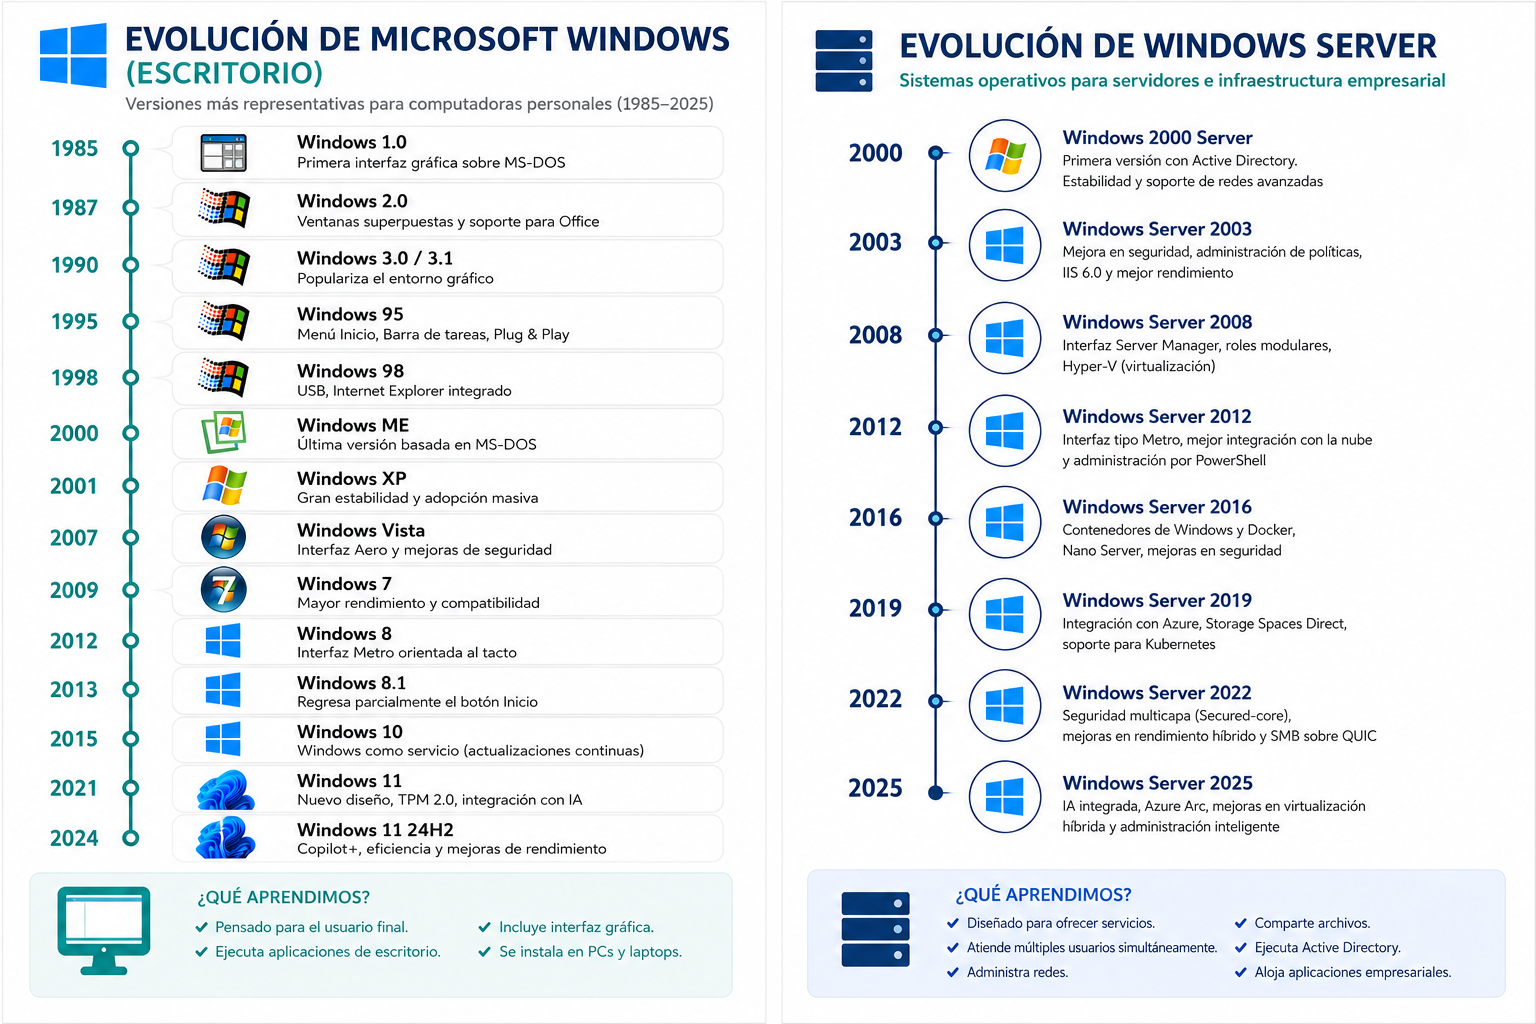
\includegraphics[width=0.82\linewidth,height=\textheight,keepaspectratio]{capitulos/../assets/img/linea_tiempo_windows_material_original.png}

}

\caption{Evolución de Windows en el material original de la clase}

\end{figure}%

\section{GNU/Linux}\label{gnulinux}

Linux es el kernel iniciado por Linus Torvalds. Cuando se combina con
herramientas, bibliotecas, gestores de paquetes y entornos de usuario,
forma sistemas completos distribuidos en variantes como Ubuntu, Debian,
Fedora, Rocky Linux, AlmaLinux o Arch Linux.

Ubuntu 24.04 LTS continúa siendo una versión de soporte prolongado
ampliamente utilizada. Las versiones LTS priorizan estabilidad y
mantenimiento extendido, una característica valiosa en organizaciones y
servidores.

\begin{tcolorbox}[enhanced jigsaw, arc=.35mm, bottomrule=.15mm, bottomtitle=1mm, breakable, colback=white, colbacktitle=quarto-callout-important-color!10!white, colframe=quarto-callout-important-color-frame, coltitle=black, left=2mm, leftrule=.75mm, opacityback=0, opacitybacktitle=0.6, rightrule=.15mm, title=\textcolor{quarto-callout-important-color}{\faExclamation}\hspace{0.5em}{Precisión terminológica}, titlerule=0mm, toprule=.15mm, toptitle=1mm]

Linux es técnicamente el kernel. En el uso cotidiano se habla de
``sistema operativo Linux'', pero una expresión más precisa para muchas
distribuciones es GNU/Linux o simplemente el nombre de la distribución:
Ubuntu, Debian, Fedora, etc.

\end{tcolorbox}

\section{macOS}\label{macos}

macOS es el sistema operativo de las computadoras Mac. A julio de 2026,
macOS Tahoe 26 es la versión estable con actualizaciones de seguridad
publicadas por Apple; macOS 27 se encuentra anunciado o en ciclo previo
a su disponibilidad general según el momento de consulta.

Para un libro reutilizable es preferible enseñar la familia, su
arquitectura general y sus herramientas, en lugar de depender únicamente
del número de versión.

\section{Android e iOS}\label{android-e-ios}

Android domina una gran variedad de dispositivos móviles y utiliza el
kernel Linux como base, aunque su entorno de aplicaciones y servicios es
diferente al de una distribución GNU/Linux de escritorio.

Android 17 fue publicado en junio de 2026. En el ecosistema Apple, iOS
26 continúa como versión estable con actualizaciones de seguridad,
mientras iOS 27 fue anunciado para una etapa posterior.

\begin{tcolorbox}[enhanced jigsaw, arc=.35mm, bottomrule=.15mm, bottomtitle=1mm, breakable, colback=white, colbacktitle=quarto-callout-tip-color!10!white, colframe=quarto-callout-tip-color-frame, coltitle=black, left=2mm, leftrule=.75mm, opacityback=0, opacitybacktitle=0.6, rightrule=.15mm, title=\textcolor{quarto-callout-tip-color}{\faLightbulb}\hspace{0.5em}{Consejo del Ingeniero}, titlerule=0mm, toprule=.15mm, toptitle=1mm]

Las versiones cambian con rapidez. En la práctica profesional, siempre
consulte la documentación oficial antes de planificar una instalación,
una actualización o una migración.

\end{tcolorbox}

\bookmarksetup{startatroot}

\chapter{Interfaces de usuario}\label{interfaces-de-usuario}

Una interfaz permite que una persona interactúe con el sistema
operativo.

\section{Interfaz gráfica de
usuario}\label{interfaz-gruxe1fica-de-usuario}

La \textbf{GUI} (\emph{Graphical User Interface}) utiliza ventanas,
iconos, menús, botones y otros elementos visuales.

Sus ventajas incluyen:

\begin{itemize}
\tightlist
\item
  facilidad de aprendizaje;
\item
  descubrimiento visual de opciones;
\item
  interacción mediante mouse, pantalla táctil o teclado;
\item
  buena experiencia para tareas generales.
\end{itemize}

\section{Interfaz de línea de
comandos}\label{interfaz-de-luxednea-de-comandos}

La \textbf{CLI} (\emph{Command-Line Interface}) permite escribir
instrucciones en una terminal o intérprete de comandos.

Entre sus ventajas se encuentran:

\begin{itemize}
\tightlist
\item
  automatización mediante scripts;
\item
  administración remota;
\item
  precisión y repetibilidad;
\item
  menor consumo de recursos en muchos escenarios;
\item
  acceso rápido a herramientas avanzadas.
\end{itemize}

\begin{figure}[H]

{\centering 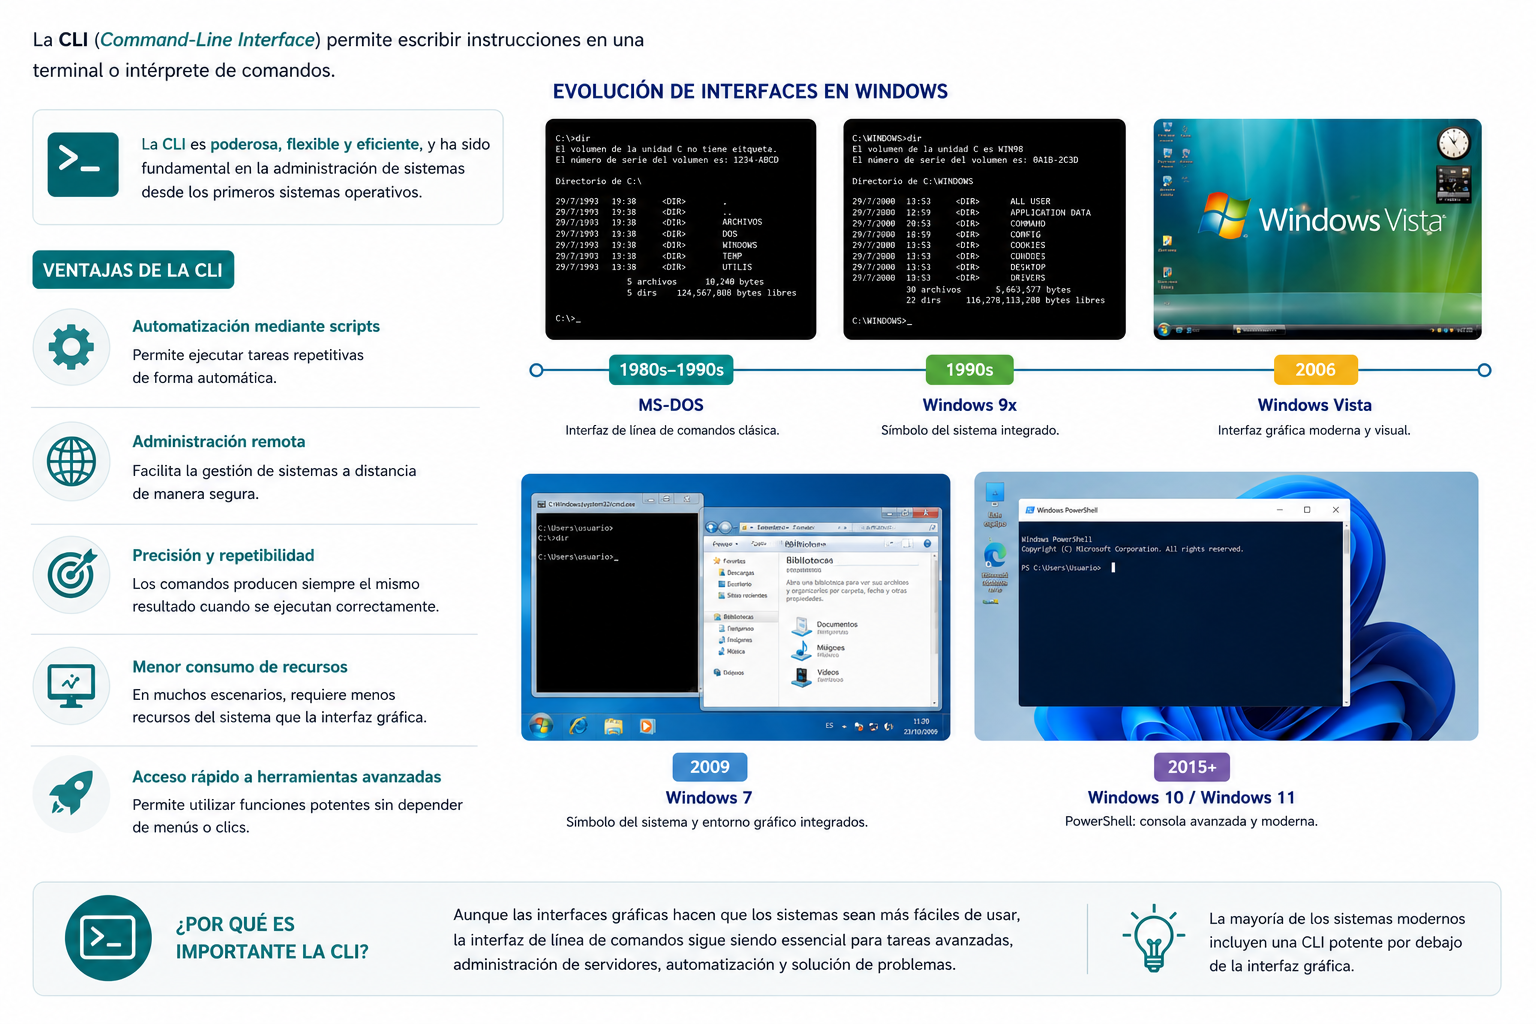
\includegraphics[width=0.85\linewidth,height=\textheight,keepaspectratio]{capitulos/../assets/img/interfaces_material_original.png}

}

\caption{Ejemplos de interfaces conservados del material original}

\end{figure}%

\section{No son enemigas}\label{no-son-enemigas}

GUI y CLI no deben verse como opciones excluyentes. Un profesional
utiliza ambas según la tarea.

{\def\LTcaptype{none} % do not increment counter
\begin{longtable}[]{@{}ll@{}}
\toprule\noalign{}
Situación & Interfaz conveniente \\
\midrule\noalign{}
\endhead
\bottomrule\noalign{}
\endlastfoot
Configurar una opción ocasional & GUI \\
Repetir la misma tarea en 100 equipos & CLI y automatización \\
Explorar visualmente archivos & GUI \\
Administrar un servidor remoto & CLI \\
Analizar procesos rápidamente & GUI o CLI, según el contexto \\
\end{longtable}
}

\begin{tcolorbox}[enhanced jigsaw, arc=.35mm, bottomrule=.15mm, bottomtitle=1mm, breakable, colback=white, colbacktitle=quarto-callout-tip-color!10!white, colframe=quarto-callout-tip-color-frame, coltitle=black, left=2mm, leftrule=.75mm, opacityback=0, opacitybacktitle=0.6, rightrule=.15mm, title=\textcolor{quarto-callout-tip-color}{\faLightbulb}\hspace{0.5em}{En la práctica profesional}, titlerule=0mm, toprule=.15mm, toptitle=1mm]

PowerShell, Bash y otras shells permiten convertir procedimientos
manuales en scripts repetibles. Esa capacidad reduce errores y facilita
administrar muchos equipos.

\end{tcolorbox}

\bookmarksetup{startatroot}

\chapter{Clasificación de los sistemas
operativos}\label{clasificaciuxf3n-de-los-sistemas-operativos}

Un sistema operativo puede pertenecer a varias categorías al mismo
tiempo.

\section{Monotarea y multitarea}\label{monotarea-y-multitarea}

\begin{itemize}
\tightlist
\item
  \textbf{Monotarea:} ejecuta una tarea principal a la vez.
\item
  \textbf{Multitarea:} administra varios procesos concurrentes y
  distribuye recursos entre ellos.
\end{itemize}

Los sistemas generales actuales son multitarea.

\section{Monousuario y multiusuario}\label{monousuario-y-multiusuario}

\begin{itemize}
\tightlist
\item
  \textbf{Monousuario:} está diseñado principalmente para una sesión o
  usuario a la vez.
\item
  \textbf{Multiusuario:} permite atender varios usuarios y separar
  recursos, permisos y sesiones.
\end{itemize}

Un servidor Linux o Windows Server puede atender múltiples usuarios y
servicios simultáneamente.

\section{Procesamiento por lotes}\label{procesamiento-por-lotes-1}

Ejecuta conjuntos de trabajos con poca interacción durante el
procesamiento. Sigue siendo útil en tareas como generación nocturna de
reportes, respaldo de información o procesamiento masivo de datos.

\section{Tiempo compartido}\label{tiempo-compartido}

Distribuye el tiempo de CPU entre múltiples usuarios o procesos
interactivos, proporcionando respuestas suficientemente rápidas para
mantener la sensación de atención individual.

\section{Sistemas de red y
distribuidos}\label{sistemas-de-red-y-distribuidos}

Un sistema operativo de red facilita compartir servicios y recursos
entre equipos conectados. Un sistema distribuido coordina componentes
ubicados en diferentes nodos para ofrecer un servicio integrado.

\section{Sistemas de tiempo real}\label{sistemas-de-tiempo-real}

Un sistema de tiempo real debe responder dentro de límites temporales
definidos.

\begin{itemize}
\tightlist
\item
  \textbf{Tiempo real duro:} incumplir el plazo puede producir una falla
  crítica.
\item
  \textbf{Tiempo real blando:} el retraso reduce la calidad del
  servicio, pero no necesariamente causa una falla catastrófica.
\end{itemize}

Ejemplos:

\begin{itemize}
\tightlist
\item
  control industrial;
\item
  sistemas automotrices;
\item
  telecomunicaciones;
\item
  robótica;
\item
  instrumentación médica;
\item
  control de energía.
\end{itemize}

\begin{figure}[H]

{\centering 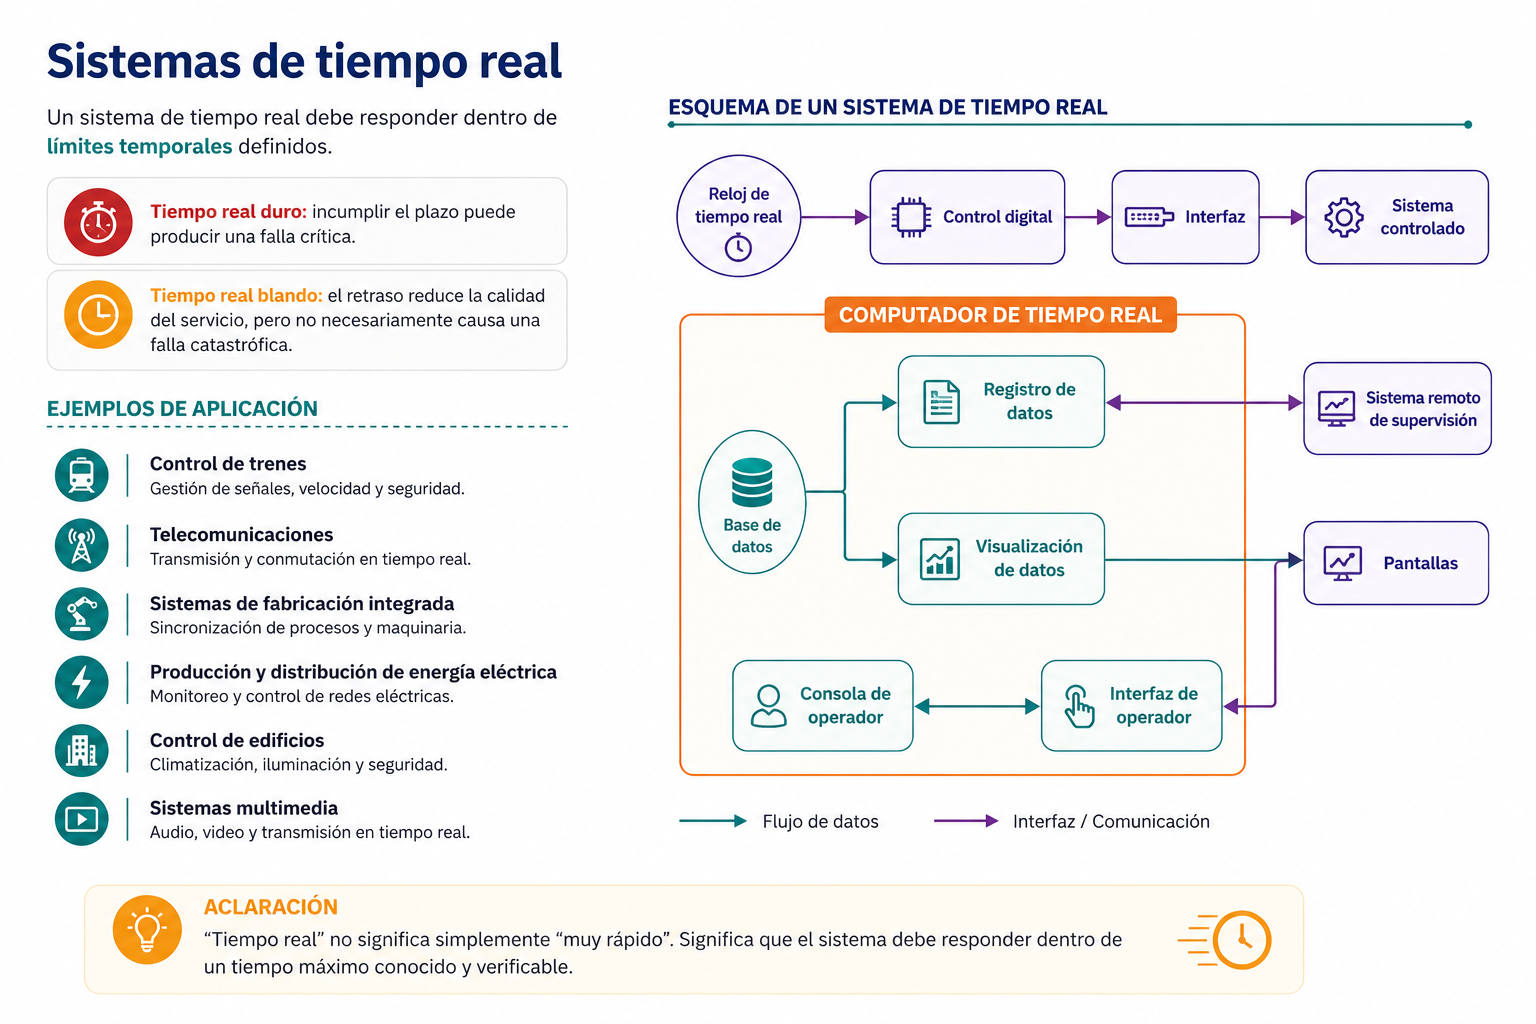
\includegraphics[width=0.72\linewidth,height=\textheight,keepaspectratio]{capitulos/../assets/img/sistema_tiempo_real_material_original.png}

}

\caption{Esquema de sistema de tiempo real tomado del material original}

\end{figure}%

\begin{tcolorbox}[enhanced jigsaw, arc=.35mm, bottomrule=.15mm, bottomtitle=1mm, breakable, colback=white, colbacktitle=quarto-callout-warning-color!10!white, colframe=quarto-callout-warning-color-frame, coltitle=black, left=2mm, leftrule=.75mm, opacityback=0, opacitybacktitle=0.6, rightrule=.15mm, title=\textcolor{quarto-callout-warning-color}{\faExclamationTriangle}\hspace{0.5em}{Aclaración}, titlerule=0mm, toprule=.15mm, toptitle=1mm]

``Tiempo real'' no significa simplemente ``muy rápido''. Significa que
el sistema debe responder dentro de un tiempo máximo conocido y
verificable.

\end{tcolorbox}

\bookmarksetup{startatroot}

\chapter{Llamadas al sistema}\label{llamadas-al-sistema}

Las aplicaciones necesitan solicitar servicios al kernel. Para hacerlo
utilizan \textbf{llamadas al sistema}.

Algunos servicios típicos son:

\begin{itemize}
\tightlist
\item
  abrir o cerrar un archivo;
\item
  crear un proceso;
\item
  reservar memoria;
\item
  comunicarse por red;
\item
  leer datos de un dispositivo;
\item
  consultar la hora del sistema.
\end{itemize}

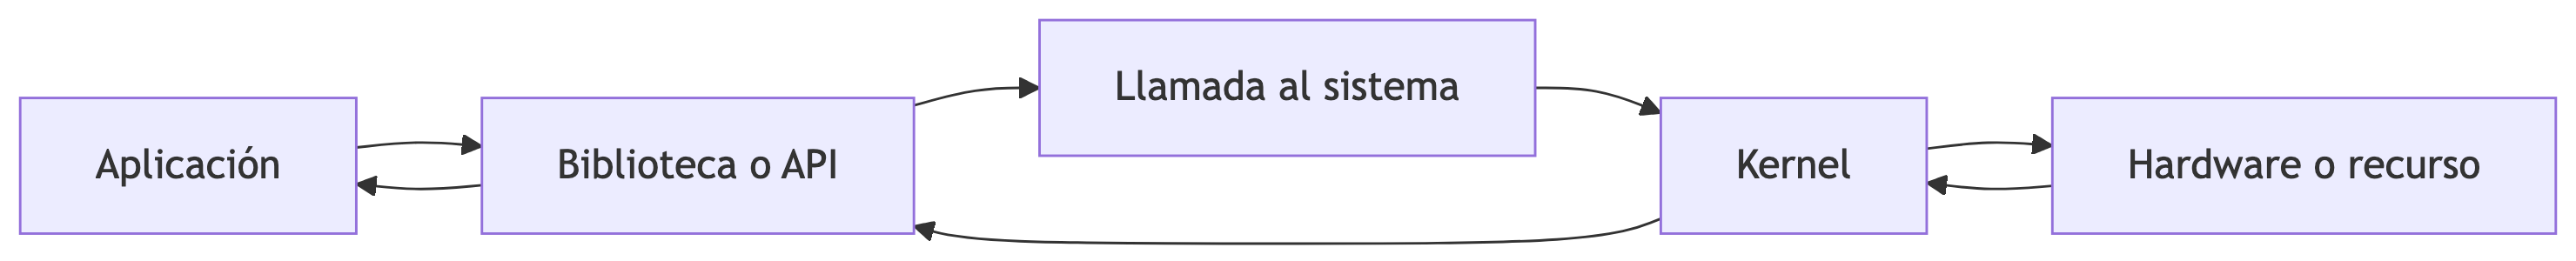
\includegraphics[width=10.68in,height=1.09in]{capitulos/01_introduccion_sistemas_operativos_files/figure-latex/mermaid-figure-1.png}

\section{Bibliotecas y API}\label{bibliotecas-y-api}

Los lenguajes de alto nivel suelen utilizar bibliotecas que presentan
funciones más sencillas. La biblioteca prepara los parámetros y realiza
la transición necesaria para solicitar el servicio al sistema operativo.

Por ejemplo, una aplicación puede llamar una función para abrir un
archivo. Esa función termina utilizando servicios del sistema operativo
para validar permisos, localizar el archivo y coordinar el acceso al
almacenamiento.

\begin{tcolorbox}[enhanced jigsaw, arc=.35mm, bottomrule=.15mm, bottomtitle=1mm, breakable, colback=white, colbacktitle=quarto-callout-note-color!10!white, colframe=quarto-callout-note-color-frame, coltitle=black, left=2mm, leftrule=.75mm, opacityback=0, opacitybacktitle=0.6, rightrule=.15mm, title=\textcolor{quarto-callout-note-color}{\faInfo}\hspace{0.5em}{Observe}, titlerule=0mm, toprule=.15mm, toptitle=1mm]

Las llamadas al sistema forman una frontera controlada entre las
aplicaciones y el kernel. Esta frontera permite ofrecer servicios sin
entregar a cada programa control total sobre el equipo.

\end{tcolorbox}

\bookmarksetup{startatroot}

\chapter{Relación con la arquitectura del
computador}\label{relaciuxf3n-con-la-arquitectura-del-computador}

Para comprender un sistema operativo también necesitamos recordar los
componentes básicos del computador.

\section{CPU}\label{cpu}

La \textbf{unidad central de procesamiento} ejecuta instrucciones y
realiza operaciones aritméticas, lógicas y de control.

En sistemas modernos, una CPU puede incluir varios núcleos, memorias
caché y mecanismos especializados. El sistema operativo planifica
procesos e hilos para aprovechar esos recursos.

\section{Memoria principal}\label{memoria-principal}

La memoria RAM almacena temporalmente instrucciones y datos necesarios
durante la ejecución.

Es rápida, pero normalmente pierde su contenido al apagar el equipo. El
sistema operativo administra qué regiones utiliza cada proceso y
coordina la memoria virtual.

\section{Almacenamiento secundario}\label{almacenamiento-secundario}

SSD, discos duros y otros medios conservan información de forma
persistente. Son más lentos que la RAM, pero poseen mayor capacidad.

\section{Unidad de control y ALU}\label{unidad-de-control-y-alu}

La unidad de control coordina la ejecución de instrucciones dentro del
procesador. La unidad aritmética y lógica realiza operaciones
matemáticas y comparaciones.

En cursos modernos estos componentes se estudian como partes de la
arquitectura del procesador, mientras el sistema operativo se analiza
como el software que administra su utilización.

\section{Periféricos y
entrada/salida}\label{perifuxe9ricos-y-entradasalida}

Teclado, mouse, pantalla, almacenamiento, impresoras y adaptadores de
red intercambian información con el sistema mediante controladores y
mecanismos de entrada/salida.

\begin{tcolorbox}[enhanced jigsaw, arc=.35mm, bottomrule=.15mm, bottomtitle=1mm, breakable, colback=white, colbacktitle=quarto-callout-tip-color!10!white, colframe=quarto-callout-tip-color-frame, coltitle=black, left=2mm, leftrule=.75mm, opacityback=0, opacitybacktitle=0.6, rightrule=.15mm, title=\textcolor{quarto-callout-tip-color}{\faLightbulb}\hspace{0.5em}{Consejo del Ingeniero}, titlerule=0mm, toprule=.15mm, toptitle=1mm]

Cuando una computadora está lenta, no asuma inmediatamente que ``la CPU
está mala''. El cuello de botella puede encontrarse en memoria,
almacenamiento, red, temperatura, controladores o en un proceso
específico.

\end{tcolorbox}

\bookmarksetup{startatroot}

\chapter{Virtualización y contenedores: una mirada
actual}\label{virtualizaciuxf3n-y-contenedores-una-mirada-actual}

La virtualización permite ejecutar máquinas virtuales con su propio
sistema operativo sobre un hipervisor.

Una máquina virtual normalmente incluye:

\begin{itemize}
\tightlist
\item
  un sistema operativo invitado;
\item
  su propio kernel;
\item
  memoria virtual asignada;
\item
  dispositivos virtuales.
\end{itemize}

Los contenedores aíslan procesos y sus dependencias, pero comparten el
kernel del sistema anfitrión. Por eso suelen ser más ligeros que una
máquina virtual completa.

{\def\LTcaptype{none} % do not increment counter
\begin{longtable}[]{@{}
  >{\raggedright\arraybackslash}p{(\linewidth - 4\tabcolsep) * \real{0.3333}}
  >{\raggedright\arraybackslash}p{(\linewidth - 4\tabcolsep) * \real{0.3333}}
  >{\raggedright\arraybackslash}p{(\linewidth - 4\tabcolsep) * \real{0.3333}}@{}}
\toprule\noalign{}
\begin{minipage}[b]{\linewidth}\raggedright
Característica
\end{minipage} & \begin{minipage}[b]{\linewidth}\raggedright
Máquina virtual
\end{minipage} & \begin{minipage}[b]{\linewidth}\raggedright
Contenedor
\end{minipage} \\
\midrule\noalign{}
\endhead
\bottomrule\noalign{}
\endlastfoot
Kernel propio & Sí & Generalmente no; comparte el kernel anfitrión \\
Aislamiento & Alto & A nivel de procesos y recursos \\
Tamaño & Mayor & Menor \\
Inicio & Más lento & Habitualmente rápido \\
Uso típico & Sistemas completos, pruebas de SO, aislamiento fuerte &
Empaquetado y despliegue de aplicaciones \\
\end{longtable}
}

\begin{tcolorbox}[enhanced jigsaw, arc=.35mm, bottomrule=.15mm, bottomtitle=1mm, breakable, colback=white, colbacktitle=quarto-callout-note-color!10!white, colframe=quarto-callout-note-color-frame, coltitle=black, left=2mm, leftrule=.75mm, opacityback=0, opacitybacktitle=0.6, rightrule=.15mm, title=\textcolor{quarto-callout-note-color}{\faInfo}\hspace{0.5em}{Primera aproximación}, titlerule=0mm, toprule=.15mm, toptitle=1mm]

Virtualización y contenedores se estudiarán con mayor profundidad más
adelante. En esta clase basta comprender que ambos dependen de funciones
esenciales del sistema operativo.

\end{tcolorbox}

\bookmarksetup{startatroot}

\chapter{Laboratorio 1: conozca su sistema
operativo}\label{laboratorio-1-conozca-su-sistema-operativo}

\section{Propósito}\label{propuxf3sito}

Identificar el sistema operativo del equipo y relacionar los conceptos
estudiados con información real.

\section{Actividad A: información
general}\label{actividad-a-informaciuxf3n-general}

Registre los siguientes datos:

{\def\LTcaptype{none} % do not increment counter
\begin{longtable}[]{@{}ll@{}}
\toprule\noalign{}
Dato & Resultado de su equipo \\
\midrule\noalign{}
\endhead
\bottomrule\noalign{}
\endlastfoot
Sistema operativo & \\
Edición o distribución & \\
Versión & \\
Arquitectura & \\
Procesador & \\
Memoria RAM & \\
Nombre del equipo & \\
Usuario actual & \\
Espacio disponible & \\
\end{longtable}
}

\section{Actividad B: Windows}\label{actividad-b-windows}

Abra \textbf{Terminal}, \textbf{PowerShell} o \textbf{Símbolo del
sistema} y ejecute:

\begin{Shaded}
\begin{Highlighting}[]
\NormalTok{systeminfo}
\end{Highlighting}
\end{Shaded}

También puede utilizar:

\begin{Shaded}
\begin{Highlighting}[]
\NormalTok{Get{-}ComputerInfo}
\end{Highlighting}
\end{Shaded}

Comandos básicos seguros para explorar:

\begin{Shaded}
\begin{Highlighting}[]
\NormalTok{hostname}
\NormalTok{whoami}
\FunctionTok{Get{-}Location}
\FunctionTok{Get{-}ChildItem}
\end{Highlighting}
\end{Shaded}

Responda:

\begin{enumerate}
\def\labelenumi{\arabic{enumi}.}
\tightlist
\item
  ¿Qué versión y compilación de Windows utiliza?
\item
  ¿Cuánta memoria física aparece instalada?
\item
  ¿Cuál es el nombre del equipo?
\item
  ¿Qué diferencia observa entre \texttt{Get-ChildItem} y la vista del
  Explorador de archivos?
\end{enumerate}

\section{Actividad C: macOS}\label{actividad-c-macos}

Abra \textbf{Terminal} y ejecute:

\begin{Shaded}
\begin{Highlighting}[]
\ExtensionTok{sw\_vers}
\FunctionTok{uname} \AttributeTok{{-}a}
\FunctionTok{whoami}
\FunctionTok{hostname}
\BuiltInTok{pwd}
\FunctionTok{ls}
\ExtensionTok{system\_profiler}\NormalTok{ SPHardwareDataType}
\end{Highlighting}
\end{Shaded}

Responda:

\begin{enumerate}
\def\labelenumi{\arabic{enumi}.}
\tightlist
\item
  ¿Qué versión de macOS utiliza?
\item
  ¿Qué arquitectura reporta el equipo?
\item
  ¿Qué información muestra \texttt{pwd}?
\item
  ¿Qué relación encuentra entre Finder y \texttt{ls}?
\end{enumerate}

\section{Actividad D: GNU/Linux}\label{actividad-d-gnulinux}

Abra una terminal y ejecute:

\begin{Shaded}
\begin{Highlighting}[]
\FunctionTok{cat}\NormalTok{ /etc/os{-}release}
\FunctionTok{uname} \AttributeTok{{-}r}
\ExtensionTok{hostnamectl}
\FunctionTok{whoami}
\BuiltInTok{pwd}
\FunctionTok{ls}
\end{Highlighting}
\end{Shaded}

Responda:

\begin{enumerate}
\def\labelenumi{\arabic{enumi}.}
\tightlist
\item
  ¿Cuál es la distribución?
\item
  ¿Qué versión del kernel utiliza?
\item
  ¿Qué arquitectura tiene el equipo?
\item
  ¿Qué información proporciona \texttt{/etc/os-release}?
\end{enumerate}

\section{Actividad E: comparación}\label{actividad-e-comparaciuxf3n}

Complete la tabla:

{\def\LTcaptype{none} % do not increment counter
\begin{longtable}[]{@{}
  >{\raggedright\arraybackslash}p{(\linewidth - 4\tabcolsep) * \real{0.3333}}
  >{\raggedright\arraybackslash}p{(\linewidth - 4\tabcolsep) * \real{0.3333}}
  >{\raggedright\arraybackslash}p{(\linewidth - 4\tabcolsep) * \real{0.3333}}@{}}
\toprule\noalign{}
\begin{minipage}[b]{\linewidth}\raggedright
Acción
\end{minipage} & \begin{minipage}[b]{\linewidth}\raggedright
Windows
\end{minipage} & \begin{minipage}[b]{\linewidth}\raggedright
macOS/Linux
\end{minipage} \\
\midrule\noalign{}
\endhead
\bottomrule\noalign{}
\endlastfoot
Mostrar usuario & \texttt{whoami} & \texttt{whoami} \\
Mostrar nombre del equipo & \texttt{hostname} & \texttt{hostname} \\
Mostrar carpeta actual & \texttt{Get-Location} & \texttt{pwd} \\
Listar archivos & \texttt{Get-ChildItem} & \texttt{ls} \\
Información del sistema & \texttt{systeminfo} & \texttt{sw\_vers},
\texttt{hostnamectl} o \texttt{/etc/os-release} \\
\end{longtable}
}

\begin{tcolorbox}[enhanced jigsaw, arc=.35mm, bottomrule=.15mm, bottomtitle=1mm, breakable, colback=white, colbacktitle=quarto-callout-warning-color!10!white, colframe=quarto-callout-warning-color-frame, coltitle=black, left=2mm, leftrule=.75mm, opacityback=0, opacitybacktitle=0.6, rightrule=.15mm, title=\textcolor{quarto-callout-warning-color}{\faExclamationTriangle}\hspace{0.5em}{Regla del laboratorio}, titlerule=0mm, toprule=.15mm, toptitle=1mm]

Ejecute únicamente los comandos indicados y lea su salida. No modifique
usuarios, permisos, particiones, fecha, hora ni configuraciones del
sistema durante esta práctica.

\end{tcolorbox}

\bookmarksetup{startatroot}

\chapter{Caso de análisis}\label{caso-de-anuxe1lisis}

Una empresa posee:

\begin{itemize}
\tightlist
\item
  40 computadoras de oficina;
\item
  un servidor de archivos;
\item
  una aplicación web;
\item
  teléfonos utilizados por personal de campo;
\item
  un sistema industrial que debe responder en milisegundos.
\end{itemize}

Analice qué tipo de sistema operativo podría utilizarse en cada contexto
y justifique su respuesta considerando:

\begin{itemize}
\tightlist
\item
  propósito;
\item
  seguridad;
\item
  administración;
\item
  interfaz;
\item
  tiempo de respuesta;
\item
  compatibilidad de aplicaciones.
\end{itemize}

\bookmarksetup{startatroot}

\chapter{Resumen de la clase}\label{resumen-de-la-clase}

En esta clase aprendimos que:

\begin{itemize}
\tightlist
\item
  El sistema operativo administra hardware y ofrece servicios a las
  aplicaciones.
\item
  El kernel es el núcleo privilegiado del sistema.
\item
  Los procesos, la memoria, los archivos, los dispositivos, la seguridad
  y la red son recursos administrados por el sistema operativo.
\item
  GUI y CLI son formas complementarias de interacción.
\item
  Los sistemas operativos pueden clasificarse por su número de tareas,
  usuarios, forma de procesamiento y requisitos temporales.
\item
  Las llamadas al sistema permiten a las aplicaciones solicitar
  servicios al kernel.
\item
  Windows, GNU/Linux, macOS, Android, iOS y los sistemas de tiempo real
  responden a necesidades distintas.
\item
  La virtualización y los contenedores dependen de capacidades
  fundamentales del sistema operativo.
\end{itemize}

\begin{tcolorbox}[enhanced jigsaw, arc=.35mm, bottomrule=.15mm, bottomtitle=1mm, breakable, colback=white, colbacktitle=quarto-callout-tip-color!10!white, colframe=quarto-callout-tip-color-frame, coltitle=black, left=2mm, leftrule=.75mm, opacityback=0, opacitybacktitle=0.6, rightrule=.15mm, title=\textcolor{quarto-callout-tip-color}{\faLightbulb}\hspace{0.5em}{Consejo final del Ingeniero}, titlerule=0mm, toprule=.15mm, toptitle=1mm]

Un buen administrador no memoriza únicamente comandos. Comprende qué
recurso está observando, qué problema intenta resolver y qué efecto
tendrá cada acción.

\end{tcolorbox}

\bookmarksetup{startatroot}

\chapter{Tarea sugerida}\label{tarea-sugerida}

\begin{enumerate}
\def\labelenumi{\arabic{enumi}.}
\tightlist
\item
  Elabore una comparación entre el sistema operativo de su computadora y
  el de su teléfono.
\item
  Identifique tres procesos activos en su equipo y explique, con sus
  propias palabras, para qué sirven.
\item
  Explique la diferencia entre kernel, sistema operativo e interfaz
  gráfica.
\item
  Investigue un ejemplo de sistema de tiempo real y explique por qué el
  cumplimiento del tiempo es importante.
\item
  Describa una situación en la que utilizaría una máquina virtual y otra
  en la que utilizaría un contenedor.
\item
  Incluya capturas de pantalla de la información obtenida en el
  laboratorio, ocultando datos personales que no desee compartir.
\end{enumerate}

\bookmarksetup{startatroot}

\chapter{Fuentes oficiales para
actualización}\label{fuentes-oficiales-para-actualizaciuxf3n}

\begin{itemize}
\tightlist
\item
  Microsoft. \emph{Windows 11 release information}:
  \url{https://learn.microsoft.com/windows/release-health/windows11-release-information}
\item
  Microsoft. \emph{Windows Server release information}:
  \url{https://learn.microsoft.com/windows/release-health/windows-server-release-info}
\item
  Apple. \emph{Apple security releases}:
  \url{https://support.apple.com/100100}
\item
  Canonical. \emph{Ubuntu release cycle}:
  \url{https://ubuntu.com/about/release-cycle}
\item
  Linux Kernel Organization. \emph{The Linux Kernel Archives}:
  \url{https://www.kernel.org/}
\item
  Android Developers. \emph{Android platform updates}:
  \url{https://developer.android.com/latest-updates}
\item
  Docker. \emph{What is a container?}:
  \url{https://docs.docker.com/get-started/docker-concepts/the-basics/what-is-a-container/}
\end{itemize}

\begin{tcolorbox}[enhanced jigsaw, arc=.35mm, bottomrule=.15mm, bottomtitle=1mm, breakable, colback=white, colbacktitle=quarto-callout-note-color!10!white, colframe=quarto-callout-note-color-frame, coltitle=black, left=2mm, leftrule=.75mm, opacityback=0, opacitybacktitle=0.6, rightrule=.15mm, title=\textcolor{quarto-callout-note-color}{\faInfo}\hspace{0.5em}{Nota editorial}, titlerule=0mm, toprule=.15mm, toptitle=1mm]

La información de versiones fue revisada en julio de 2026. Debido a que
los sistemas operativos se actualizan continuamente, las versiones
exactas deben verificarse en la documentación oficial al impartir
nuevamente la clase.

\end{tcolorbox}

\bookmarksetup{startatroot}

\chapter{Administración del sistema de archivos desde la línea de
comandos}\label{administraciuxf3n-del-sistema-de-archivos-desde-la-luxednea-de-comandos}

Clase 2

\hfill\break

\bookmarksetup{startatroot}

\chapter{Presentación de la clase}\label{presentaciuxf3n-de-la-clase-1}

En la clase anterior estudiamos qué es un sistema operativo y por qué
constituye la base de todo sistema informático. En esta sesión nos
concentraremos en una de sus funciones más visibles: \textbf{organizar y
administrar la información almacenada}.

Cada documento, fotografía, programa o proyecto necesita un lugar dentro
del sistema. Cuando esa información está bien organizada, puede
localizarse, copiarse, trasladarse o eliminarse con rapidez. Cuando no
lo está, incluso un archivo que sigue existiendo puede parecer perdido.

La administración de archivos puede realizarse mediante ventanas e
iconos, pero también a través de instrucciones escritas. Por ello, en
esta clase utilizaremos el \textbf{Símbolo del sistema de Windows (CMD)}
para comprender cómo piensa el sistema operativo cuando trabaja con
unidades, directorios, rutas y archivos.

\begin{tcolorbox}[enhanced jigsaw, arc=.35mm, bottomrule=.15mm, bottomtitle=1mm, breakable, colback=white, colbacktitle=quarto-callout-note-color!10!white, colframe=quarto-callout-note-color-frame, coltitle=black, left=2mm, leftrule=.75mm, opacityback=0, opacitybacktitle=0.6, rightrule=.15mm, title=\textcolor{quarto-callout-note-color}{\faInfo}\hspace{0.5em}{Idea central}, titlerule=0mm, toprule=.15mm, toptitle=1mm]

Los comandos no son palabras aisladas para memorizar. Son instrucciones
que expresan una necesidad concreta: ver, entrar, crear, copiar, mover,
renombrar o eliminar.

\end{tcolorbox}

\section{Objetivos de aprendizaje}\label{objetivos-de-aprendizaje-1}

Al finalizar esta clase, el estudiante será capaz de:

\begin{itemize}
\tightlist
\item
  Explicar cómo organiza el sistema operativo la información.
\item
  Diferenciar unidades, directorios, subdirectorios y archivos.
\item
  Interpretar rutas absolutas y relativas.
\item
  Reconocer la función del intérprete de comandos de Windows.
\item
  Utilizar comandos básicos para navegar y organizar información.
\item
  Aplicar buenas prácticas para evitar errores durante la administración
  de archivos.
\end{itemize}

\section{Ruta de trabajo de la
sesión}\label{ruta-de-trabajo-de-la-sesiuxf3n}

{\def\LTcaptype{none} % do not increment counter
\begin{longtable}[]{@{}llr@{}}
\toprule\noalign{}
Momento & Actividad & Tiempo aproximado \\
\midrule\noalign{}
\endhead
\bottomrule\noalign{}
\endlastfoot
Inicio & Situación problemática y conceptos base & 15 min \\
Desarrollo & Directorios, archivos, rutas y CMD & 20 min \\
Laboratorio & Construcción del proyecto \texttt{SOI} & 35 min \\
Aplicación & Reto guiado y análisis de errores & 15 min \\
Cierre & Síntesis y autoevaluación & 5 min \\
\end{longtable}
}

\bookmarksetup{startatroot}

\chapter{¿Dónde está realmente un
archivo?}\label{duxf3nde-estuxe1-realmente-un-archivo}

Imagine que debe entregar un proyecto al finalizar la clase. Está seguro
de haberlo guardado, pero no recuerda si quedó en \textbf{Documentos},
\textbf{Descargas}, \textbf{Escritorio} o una memoria USB.

El archivo no necesariamente se perdió. El problema puede ser que
desconoce su ubicación.

Los sistemas operativos resuelven esta situación mediante una
organización jerárquica. En lugar de almacenar toda la información en un
único espacio, la distribuyen en unidades, directorios y subdirectorios.

\begin{figure}

\centering{


\includegraphics[width=0.88\linewidth,height=\textheight,keepaspectratio]{index_files/mediabag/capitulos/../img/clase_02/fig_02_01_jerarquia.pdf}

}

\caption{\label{fig-jerarquia}Organización jerárquica del sistema de
archivos}

\end{figure}%

En esta estructura:

\begin{itemize}
\tightlist
\item
  La \textbf{unidad} representa un dispositivo o volumen de
  almacenamiento.
\item
  El \textbf{directorio} agrupa información relacionada.
\item
  El \textbf{subdirectorio} es un directorio ubicado dentro de otro.
\item
  El \textbf{archivo} contiene los datos que utiliza el usuario o una
  aplicación.
\end{itemize}

\begin{tcolorbox}[enhanced jigsaw, arc=.35mm, bottomrule=.15mm, bottomtitle=1mm, breakable, colback=white, colbacktitle=quarto-callout-tip-color!10!white, colframe=quarto-callout-tip-color-frame, coltitle=black, left=2mm, leftrule=.75mm, opacityback=0, opacitybacktitle=0.6, rightrule=.15mm, title=\textcolor{quarto-callout-tip-color}{\faLightbulb}\hspace{0.5em}{Consejo del Ingeniero}, titlerule=0mm, toprule=.15mm, toptitle=1mm]

Un archivo bien nombrado y guardado en una estructura lógica puede
ahorrar más tiempo que cualquier comando avanzado.

\end{tcolorbox}

\bookmarksetup{startatroot}

\chapter{El sistema de archivos}\label{el-sistema-de-archivos}

Un \textbf{sistema de archivos} es el conjunto de reglas y estructuras
que utiliza el sistema operativo para registrar, organizar, localizar y
proteger la información dentro de un dispositivo de almacenamiento.

El usuario observa carpetas y nombres. Internamente, el sistema
operativo también mantiene datos como:

\begin{itemize}
\tightlist
\item
  ubicación lógica;
\item
  tamaño;
\item
  fecha de creación y modificación;
\item
  permisos;
\item
  atributos;
\item
  relación entre directorios y archivos.
\end{itemize}

La organización lógica evita que el usuario deba conocer el lugar físico
exacto donde se encuentran los datos dentro del dispositivo.

\section{Unidades de almacenamiento}\label{unidades-de-almacenamiento}

En Windows, las unidades suelen identificarse mediante una letra seguida
de dos puntos:

\begin{Shaded}
\begin{Highlighting}[]
\NormalTok{C:}
\NormalTok{D:}
\NormalTok{E:}
\end{Highlighting}
\end{Shaded}

La unidad \texttt{C:} suele contener el sistema operativo y los perfiles
de usuario. Otras letras pueden representar particiones, memorias USB,
discos externos, unidades ópticas o recursos conectados.

\begin{tcolorbox}[enhanced jigsaw, arc=.35mm, bottomrule=.15mm, bottomtitle=1mm, breakable, colback=white, colbacktitle=quarto-callout-warning-color!10!white, colframe=quarto-callout-warning-color-frame, coltitle=black, left=2mm, leftrule=.75mm, opacityback=0, opacitybacktitle=0.6, rightrule=.15mm, title=\textcolor{quarto-callout-warning-color}{\faExclamationTriangle}\hspace{0.5em}{No confundir}, titlerule=0mm, toprule=.15mm, toptitle=1mm]

La letra no indica por sí sola el tipo de dispositivo. Una memoria USB
puede aparecer como \texttt{D:}, \texttt{E:} o cualquier otra letra
disponible.

\end{tcolorbox}

\section{Directorios y carpetas}\label{directorios-y-carpetas}

En Windows se utiliza con frecuencia la palabra \textbf{carpeta}. En el
lenguaje técnico y en la línea de comandos se emplea el término
\textbf{directorio}.

Ambos describen una estructura que permite agrupar archivos y otros
directorios.

\begin{Shaded}
\begin{Highlighting}[]
\NormalTok{C:\textbackslash{}}
\NormalTok{└── Usuarios}
\NormalTok{    └── Estudiante}
\NormalTok{        ├── Documentos}
\NormalTok{        ├── Descargas}
\NormalTok{        └── Escritorio}
\end{Highlighting}
\end{Shaded}

\section{Archivos y extensiones}\label{archivos-y-extensiones}

Un archivo es una unidad de información identificada mediante un nombre.

\begin{Shaded}
\begin{Highlighting}[]
\NormalTok{informe.docx}
\NormalTok{presupuesto.xlsx}
\NormalTok{programa.cpp}
\NormalTok{manual.pdf}
\NormalTok{imagen.png}
\end{Highlighting}
\end{Shaded}

La parte ubicada después del último punto se denomina
\textbf{extensión}. Esta ayuda al sistema operativo y a las aplicaciones
a reconocer el formato del archivo.

\begin{tcolorbox}[enhanced jigsaw, arc=.35mm, bottomrule=.15mm, bottomtitle=1mm, breakable, colback=white, colbacktitle=quarto-callout-important-color!10!white, colframe=quarto-callout-important-color-frame, coltitle=black, left=2mm, leftrule=.75mm, opacityback=0, opacitybacktitle=0.6, rightrule=.15mm, title=\textcolor{quarto-callout-important-color}{\faExclamation}\hspace{0.5em}{Idea clave}, titlerule=0mm, toprule=.15mm, toptitle=1mm]

Cambiar \texttt{fotografia.jpg} por \texttt{fotografia.pdf} no
transforma la imagen en un PDF. Solo modifica el nombre.

\end{tcolorbox}

\bookmarksetup{startatroot}

\chapter{Rutas: la dirección de la
información}\label{rutas-la-direcciuxf3n-de-la-informaciuxf3n}

Una \textbf{ruta} indica la ubicación de un archivo o directorio dentro
de la jerarquía del sistema.

\begin{figure}

\centering{


\includegraphics[width=0.92\linewidth,height=\textheight,keepaspectratio]{index_files/mediabag/capitulos/../img/clase_02/fig_02_02_rutas.pdf}

}

\caption{\label{fig-rutas}Ruta absoluta y ruta relativa}

\end{figure}%

\section{Ruta absoluta}\label{ruta-absoluta}

Una ruta absoluta comienza desde la unidad y describe el recorrido
completo.

\begin{Shaded}
\begin{Highlighting}[]
\NormalTok{C:\textbackslash{}Usuarios\textbackslash{}Estudiante\textbackslash{}Documentos\textbackslash{}SOI\textbackslash{}Clase\_02\textbackslash{}notas.txt}
\end{Highlighting}
\end{Shaded}

Esta ruta puede interpretarse de izquierda a derecha:

\begin{enumerate}
\def\labelenumi{\arabic{enumi}.}
\tightlist
\item
  Unidad \texttt{C:}.
\item
  Directorio \texttt{Usuarios}.
\item
  Perfil \texttt{Estudiante}.
\item
  Directorio \texttt{Documentos}.
\item
  Proyecto \texttt{SOI}.
\item
  Directorio \texttt{Clase\_02}.
\item
  Archivo \texttt{notas.txt}.
\end{enumerate}

\section{Ruta relativa}\label{ruta-relativa}

Una ruta relativa se interpreta desde la ubicación actual.

Si la ubicación actual es:

\begin{Shaded}
\begin{Highlighting}[]
\NormalTok{C:\textbackslash{}Usuarios\textbackslash{}Estudiante\textbackslash{}Documentos\textbackslash{}SOI}
\end{Highlighting}
\end{Shaded}

la ruta relativa hacia el archivo anterior sería:

\begin{Shaded}
\begin{Highlighting}[]
\NormalTok{Clase\_02\textbackslash{}notas.txt}
\end{Highlighting}
\end{Shaded}

El símbolo \texttt{..} representa el directorio superior.

\begin{Shaded}
\begin{Highlighting}[]
\NormalTok{cd ..}
\end{Highlighting}
\end{Shaded}

significa:

\begin{quote}
Subir un nivel dentro de la estructura.
\end{quote}

\section{Separadores y espacios}\label{separadores-y-espacios}

Windows utiliza la barra invertida \texttt{\textbackslash{}} para
separar los componentes de una ruta.

Cuando una ruta contiene espacios, es recomendable escribirla entre
comillas:

\begin{Shaded}
\begin{Highlighting}[]
\NormalTok{cd "C:\textbackslash{}Usuarios\textbackslash{}Estudiante\textbackslash{}Mis documentos"}
\end{Highlighting}
\end{Shaded}

\bookmarksetup{startatroot}

\chapter{De la interfaz gráfica a la línea de
comandos}\label{de-la-interfaz-gruxe1fica-a-la-luxednea-de-comandos}

La interfaz gráfica permite administrar información mediante ventanas,
iconos, menús y el puntero. La interfaz de línea de comandos permite
hacerlo escribiendo instrucciones.

{\def\LTcaptype{none} % do not increment counter
\begin{longtable}[]{@{}ll@{}}
\toprule\noalign{}
Interfaz gráfica & Línea de comandos \\
\midrule\noalign{}
\endhead
\bottomrule\noalign{}
\endlastfoot
Utiliza ventanas e iconos & Utiliza instrucciones escritas \\
Es visual e intuitiva & Es precisa y reproducible \\
Facilita tareas ocasionales & Facilita automatización y diagnóstico \\
Requiere navegación manual & Puede ejecutar secuencias rápidamente \\
\end{longtable}
}

Ninguna reemplaza completamente a la otra. Un profesional utiliza la
herramienta más adecuada para cada situación.

\bookmarksetup{startatroot}

\chapter{¿Qué es un comando?}\label{quuxe9-es-un-comando}

Un \textbf{comando} es una instrucción que el usuario entrega a un
intérprete para solicitar una acción.

Ejemplos:

\begin{Shaded}
\begin{Highlighting}[]
\BuiltInTok{dir}
\end{Highlighting}
\end{Shaded}

Solicita mostrar el contenido del directorio actual.

\begin{Shaded}
\begin{Highlighting}[]
\BuiltInTok{mkdir}\NormalTok{ Clase\_02}
\end{Highlighting}
\end{Shaded}

Solicita crear un directorio llamado \texttt{Clase\_02}.

\begin{Shaded}
\begin{Highlighting}[]
\BuiltInTok{copy}\NormalTok{ notas.txt respaldo.txt}
\end{Highlighting}
\end{Shaded}

Solicita crear una copia del archivo.

Los comandos pueden aceptar:

\begin{itemize}
\tightlist
\item
  \textbf{argumentos}, que indican sobre qué elemento trabajar;
\item
  \textbf{opciones}, que modifican la forma en que se ejecuta la
  instrucción.
\end{itemize}

Ejemplo:

\begin{Shaded}
\begin{Highlighting}[]
\BuiltInTok{dir} \AttributeTok{/w}
\end{Highlighting}
\end{Shaded}

\begin{itemize}
\tightlist
\item
  \texttt{dir} es el comando.
\item
  \texttt{/w} es una opción que muestra una vista resumida.
\end{itemize}

\bookmarksetup{startatroot}

\chapter{CMD en Windows}\label{cmd-en-windows}

El \textbf{Símbolo del sistema}, también conocido como \textbf{CMD}, es
un intérprete de comandos incluido en Windows.

No debe confundirse con MS-DOS. Aunque conserva numerosos comandos
históricos, CMD funciona dentro de Windows y utiliza los servicios del
sistema operativo actual.

\section{Cómo abrirlo}\label{cuxf3mo-abrirlo}

Puede abrirse de distintas maneras:

\begin{enumerate}
\def\labelenumi{\arabic{enumi}.}
\tightlist
\item
  Presionar la tecla Windows.
\item
  Escribir \texttt{cmd}.
\item
  Seleccionar \textbf{Símbolo del sistema}.
\end{enumerate}

También puede utilizarse la ventana \textbf{Ejecutar}:

\begin{Shaded}
\begin{Highlighting}[]
\NormalTok{Windows + R}
\end{Highlighting}
\end{Shaded}

Luego escribir:

\begin{Shaded}
\begin{Highlighting}[]
\NormalTok{cmd}
\end{Highlighting}
\end{Shaded}

y presionar Enter.

\begin{tcolorbox}[enhanced jigsaw, arc=.35mm, bottomrule=.15mm, bottomtitle=1mm, breakable, colback=white, colbacktitle=quarto-callout-warning-color!10!white, colframe=quarto-callout-warning-color-frame, coltitle=black, left=2mm, leftrule=.75mm, opacityback=0, opacitybacktitle=0.6, rightrule=.15mm, title=\textcolor{quarto-callout-warning-color}{\faExclamationTriangle}\hspace{0.5em}{Permisos administrativos}, titlerule=0mm, toprule=.15mm, toptitle=1mm]

Para esta práctica no es necesario abrir CMD como administrador.
Trabajar con privilegios elevados aumenta el impacto de un error.

\end{tcolorbox}

\bookmarksetup{startatroot}

\chapter{Anatomía del prompt}\label{anatomuxeda-del-prompt}

Al abrir CMD aparece una línea similar a:

\begin{Shaded}
\begin{Highlighting}[]
\NormalTok{C:\textbackslash{}Users\textbackslash{}Estudiante\textgreater{}}
\end{Highlighting}
\end{Shaded}

\begin{figure}

\centering{


\includegraphics[width=0.88\linewidth,height=\textheight,keepaspectratio]{index_files/mediabag/capitulos/../img/clase_02/fig_02_03_prompt.pdf}

}

\caption{\label{fig-prompt}Anatomía del prompt de CMD}

\end{figure}%

El prompt muestra la ubicación actual y termina con el símbolo
\texttt{\textgreater{}} para indicar que el intérprete espera una
instrucción.

\begin{Shaded}
\begin{Highlighting}[]
\NormalTok{C:                         unidad}
\NormalTok{\textbackslash{}Users\textbackslash{}Estudiante          ruta actual}
\NormalTok{\textgreater{}                          espera un comando}
\end{Highlighting}
\end{Shaded}

\begin{tcolorbox}[enhanced jigsaw, arc=.35mm, bottomrule=.15mm, bottomtitle=1mm, breakable, colback=white, colbacktitle=quarto-callout-note-color!10!white, colframe=quarto-callout-note-color-frame, coltitle=black, left=2mm, leftrule=.75mm, opacityback=0, opacitybacktitle=0.6, rightrule=.15mm, title=\textcolor{quarto-callout-note-color}{\faInfo}\hspace{0.5em}{Observe}, titlerule=0mm, toprule=.15mm, toptitle=1mm]

Cada vez que cambia de directorio, el prompt también cambia. Por eso
funciona como una brújula dentro del sistema de archivos.

\end{tcolorbox}

\bookmarksetup{startatroot}

\chapter{Laboratorio narrativo: construyendo el proyecto
SOI}\label{laboratorio-narrativo-construyendo-el-proyecto-soi}

\section{Situación}\label{situaciuxf3n}

Durante el semestre se generarán apuntes, prácticas, recursos y
entregables. Para evitar que todo quede mezclado, construiremos una
estructura permanente llamada \texttt{SOI}.

El laboratorio se realizará dentro de \textbf{Documentos}. No trabaje en
directorios del sistema como \texttt{C:\textbackslash{}Windows} o
\texttt{C:\textbackslash{}Program\ Files}.

\section{Paso 1. Saber dónde
estamos}\label{paso-1.-saber-duxf3nde-estamos}

Escriba:

\begin{Shaded}
\begin{Highlighting}[]
\BuiltInTok{cd}
\end{Highlighting}
\end{Shaded}

CMD mostrará la ruta actual.

También puede observarla directamente en el prompt.

\section{Paso 2. Ver el contenido}\label{paso-2.-ver-el-contenido}

Ejecute:

\begin{Shaded}
\begin{Highlighting}[]
\BuiltInTok{dir}
\end{Highlighting}
\end{Shaded}

El comando \texttt{dir} muestra directorios y archivos de la ubicación
actual.

En la salida encontrará datos como:

\begin{itemize}
\tightlist
\item
  fecha y hora;
\item
  indicador \texttt{\textless{}DIR\textgreater{}} para directorios;
\item
  tamaño de archivos;
\item
  nombre de cada elemento.
\end{itemize}

\subsection{Variantes útiles}\label{variantes-uxfatiles}

\begin{Shaded}
\begin{Highlighting}[]
\BuiltInTok{dir} \AttributeTok{/w}
\end{Highlighting}
\end{Shaded}

Muestra una vista resumida.

\begin{Shaded}
\begin{Highlighting}[]
\BuiltInTok{dir} \AttributeTok{/p}
\end{Highlighting}
\end{Shaded}

Pausa la salida cuando ocupa más de una pantalla.

\begin{Shaded}
\begin{Highlighting}[]
\BuiltInTok{dir}\NormalTok{ *.txt}
\end{Highlighting}
\end{Shaded}

Muestra únicamente archivos con extensión \texttt{.txt}.

\begin{tcolorbox}[enhanced jigsaw, arc=.35mm, bottomrule=.15mm, bottomtitle=1mm, breakable, colback=white, colbacktitle=quarto-callout-tip-color!10!white, colframe=quarto-callout-tip-color-frame, coltitle=black, left=2mm, leftrule=.75mm, opacityback=0, opacitybacktitle=0.6, rightrule=.15mm, title=\textcolor{quarto-callout-tip-color}{\faLightbulb}\hspace{0.5em}{Lectura antes de acción}, titlerule=0mm, toprule=.15mm, toptitle=1mm]

Antes de crear, mover o borrar algo, use \texttt{dir}. Confirmar la
ubicación reduce errores.

\end{tcolorbox}

\section{Paso 3. Ir a Documentos}\label{paso-3.-ir-a-documentos}

Según el idioma y la configuración de Windows, el nombre visible puede
variar. Una forma práctica es utilizar la variable del perfil:

\begin{Shaded}
\begin{Highlighting}[]
\BuiltInTok{cd} \AttributeTok{/d} \StringTok{"}\PreprocessorTok{\%}\VariableTok{USERPROFILE}\PreprocessorTok{\%}\StringTok{\textbackslash{}Documents"}
\end{Highlighting}
\end{Shaded}

Si la carpeta se muestra en español pero la ruta interna utiliza
\texttt{Documents}, el comando seguirá funcionando.

La opción \texttt{/d} permite cambiar de unidad y directorio en una sola
instrucción.

\section{Paso 4. Crear el directorio
principal}\label{paso-4.-crear-el-directorio-principal}

\begin{Shaded}
\begin{Highlighting}[]
\BuiltInTok{mkdir}\NormalTok{ SOI}
\end{Highlighting}
\end{Shaded}

También puede utilizarse la forma abreviada:

\begin{Shaded}
\begin{Highlighting}[]
\BuiltInTok{md}\NormalTok{ SOI}
\end{Highlighting}
\end{Shaded}

Ambos comandos crean el directorio.

Compruebe el resultado:

\begin{Shaded}
\begin{Highlighting}[]
\BuiltInTok{dir}
\end{Highlighting}
\end{Shaded}

\section{Paso 5. Entrar al proyecto}\label{paso-5.-entrar-al-proyecto}

\begin{Shaded}
\begin{Highlighting}[]
\BuiltInTok{cd}\NormalTok{ SOI}
\end{Highlighting}
\end{Shaded}

El prompt debería terminar de forma similar a:

\begin{Shaded}
\begin{Highlighting}[]
\NormalTok{...\textbackslash{}Documents\textbackslash{}SOI\textgreater{}}
\end{Highlighting}
\end{Shaded}

\section{Paso 6. Crear la estructura del
semestre}\label{paso-6.-crear-la-estructura-del-semestre}

Ejecute:

\begin{Shaded}
\begin{Highlighting}[]
\BuiltInTok{mkdir}\NormalTok{ Clase\_01 Clase\_02 Clase\_03 Laboratorios Recursos Proyecto\_Final}
\end{Highlighting}
\end{Shaded}

Luego verifique:

\begin{Shaded}
\begin{Highlighting}[]
\BuiltInTok{dir}
\end{Highlighting}
\end{Shaded}

La estructura esperada es:

\begin{Shaded}
\begin{Highlighting}[]
\NormalTok{SOI}
\NormalTok{├── Clase\_01}
\NormalTok{├── Clase\_02}
\NormalTok{├── Clase\_03}
\NormalTok{├── Laboratorios}
\NormalTok{├── Recursos}
\NormalTok{└── Proyecto\_Final}
\end{Highlighting}
\end{Shaded}

\begin{figure}

\centering{


\includegraphics[width=0.84\linewidth,height=\textheight,keepaspectratio]{index_files/mediabag/capitulos/../img/clase_02/fig_02_04_proyecto_soi.pdf}

}

\caption{\label{fig-proyecto}Estructura inicial del proyecto SOI}

\end{figure}%

\section{Paso 7. Visualizar el
árbol}\label{paso-7.-visualizar-el-uxe1rbol}

Ejecute:

\begin{Shaded}
\begin{Highlighting}[]
\KeywordTok{tree}
\end{Highlighting}
\end{Shaded}

Para incluir también archivos:

\begin{Shaded}
\begin{Highlighting}[]
\KeywordTok{tree} \AttributeTok{/f}
\end{Highlighting}
\end{Shaded}

\texttt{tree} permite comprobar visualmente la jerarquía construida.

\bookmarksetup{startatroot}

\chapter{\texorpdfstring{Navegación con
\texttt{cd}}{Navegación con cd}}\label{navegaciuxf3n-con-cd}

El comando \texttt{cd} significa \textbf{change directory}, es decir,
cambiar de directorio.

\section{Entrar a un directorio}\label{entrar-a-un-directorio}

\begin{Shaded}
\begin{Highlighting}[]
\BuiltInTok{cd}\NormalTok{ Clase\_02}
\end{Highlighting}
\end{Shaded}

\section{Subir un nivel}\label{subir-un-nivel}

\begin{Shaded}
\begin{Highlighting}[]
\BuiltInTok{cd}\NormalTok{ ..}
\end{Highlighting}
\end{Shaded}

\section{Ir a la raíz de la unidad}\label{ir-a-la-rauxedz-de-la-unidad}

\begin{Shaded}
\begin{Highlighting}[]
\BuiltInTok{cd} \SpecialCharTok{\textbackslash{}}
\end{Highlighting}
\end{Shaded}

\section{Cambiar directamente mediante una
ruta}\label{cambiar-directamente-mediante-una-ruta}

\begin{Shaded}
\begin{Highlighting}[]
\BuiltInTok{cd} \AttributeTok{/d} \StringTok{"}\PreprocessorTok{\%}\VariableTok{USERPROFILE}\PreprocessorTok{\%}\StringTok{\textbackslash{}Documents\textbackslash{}SOI\textbackslash{}Clase\_02"}
\end{Highlighting}
\end{Shaded}

\section{Volver al directorio
anterior}\label{volver-al-directorio-anterior}

CMD no ofrece exactamente el mismo comportamiento que algunos
intérpretes modernos, por lo que conviene leer el prompt y utilizar
rutas relativas o absolutas de manera consciente.

\begin{tcolorbox}[enhanced jigsaw, arc=.35mm, bottomrule=.15mm, bottomtitle=1mm, breakable, colback=white, colbacktitle=quarto-callout-warning-color!10!white, colframe=quarto-callout-warning-color-frame, coltitle=black, left=2mm, leftrule=.75mm, opacityback=0, opacitybacktitle=0.6, rightrule=.15mm, title=\textcolor{quarto-callout-warning-color}{\faExclamationTriangle}\hspace{0.5em}{Error común}, titlerule=0mm, toprule=.15mm, toptitle=1mm]

\texttt{cd...} no es la forma correcta de subir un nivel. Debe existir
un espacio:

\begin{Shaded}
\begin{Highlighting}[]
\BuiltInTok{cd}\NormalTok{ ..}
\end{Highlighting}
\end{Shaded}

\end{tcolorbox}

\bookmarksetup{startatroot}

\chapter{Crear archivos de
práctica}\label{crear-archivos-de-pruxe1ctica}

Para continuar necesitamos archivos sencillos.

Ubíquese dentro de \texttt{Clase\_02}:

\begin{Shaded}
\begin{Highlighting}[]
\BuiltInTok{cd} \AttributeTok{/d} \StringTok{"}\PreprocessorTok{\%}\VariableTok{USERPROFILE}\PreprocessorTok{\%}\StringTok{\textbackslash{}Documents\textbackslash{}SOI\textbackslash{}Clase\_02"}
\end{Highlighting}
\end{Shaded}

Cree un archivo de texto:

\begin{Shaded}
\begin{Highlighting}[]
\BuiltInTok{echo}\NormalTok{ Apuntes de la Clase 2 }\KeywordTok{\textgreater{}}\NormalTok{ apuntes.txt}
\end{Highlighting}
\end{Shaded}

Agregue una segunda línea:

\begin{Shaded}
\begin{Highlighting}[]
\BuiltInTok{echo}\NormalTok{ Practica de comandos de Windows }\KeywordTok{\textgreater{}\textgreater{}}\NormalTok{ apuntes.txt}
\end{Highlighting}
\end{Shaded}

Los operadores utilizados son:

\begin{itemize}
\tightlist
\item
  \texttt{\textgreater{}} crea o reemplaza el contenido.
\item
  \texttt{\textgreater{}\textgreater{}} agrega contenido al final.
\end{itemize}

Compruebe el archivo:

\begin{Shaded}
\begin{Highlighting}[]
\BuiltInTok{dir}
\end{Highlighting}
\end{Shaded}

Muestre su contenido:

\begin{Shaded}
\begin{Highlighting}[]
\BuiltInTok{type}\NormalTok{ apuntes.txt}
\end{Highlighting}
\end{Shaded}

\begin{tcolorbox}[enhanced jigsaw, arc=.35mm, bottomrule=.15mm, bottomtitle=1mm, breakable, colback=white, colbacktitle=quarto-callout-important-color!10!white, colframe=quarto-callout-important-color-frame, coltitle=black, left=2mm, leftrule=.75mm, opacityback=0, opacitybacktitle=0.6, rightrule=.15mm, title=\textcolor{quarto-callout-important-color}{\faExclamation}\hspace{0.5em}{Precaución}, titlerule=0mm, toprule=.15mm, toptitle=1mm]

El operador \texttt{\textgreater{}} reemplaza el contenido existente.
Antes de usarlo sobre un archivo importante, compruebe el nombre y la
ruta.

\end{tcolorbox}

\bookmarksetup{startatroot}

\chapter{\texorpdfstring{Copiar archivos con
\texttt{copy}}{Copiar archivos con copy}}\label{copiar-archivos-con-copy}

El comando \texttt{copy} crea una copia de uno o varios archivos.

\section{Copiar en el mismo
directorio}\label{copiar-en-el-mismo-directorio}

\begin{Shaded}
\begin{Highlighting}[]
\BuiltInTok{copy}\NormalTok{ apuntes.txt respaldo\_apuntes.txt}
\end{Highlighting}
\end{Shaded}

\section{Copiar hacia otro
directorio}\label{copiar-hacia-otro-directorio}

\begin{Shaded}
\begin{Highlighting}[]
\BuiltInTok{copy}\NormalTok{ apuntes.txt ..\textbackslash{}Recursos\textbackslash{}}
\end{Highlighting}
\end{Shaded}

La ruta \texttt{..\textbackslash{}Recursos\textbackslash{}} significa:

\begin{enumerate}
\def\labelenumi{\arabic{enumi}.}
\tightlist
\item
  subir desde \texttt{Clase\_02} hacia \texttt{SOI};
\item
  entrar en \texttt{Recursos}.
\end{enumerate}

Compruebe el resultado:

\begin{Shaded}
\begin{Highlighting}[]
\BuiltInTok{dir}\NormalTok{ ..\textbackslash{}Recursos}
\end{Highlighting}
\end{Shaded}

\section{Evitar sobrescrituras
accidentales}\label{evitar-sobrescrituras-accidentales}

Puede utilizar:

\begin{Shaded}
\begin{Highlighting}[]
\BuiltInTok{copy}\NormalTok{ /}\AttributeTok{{-}y}\NormalTok{ apuntes.txt respaldo\_apuntes.txt}
\end{Highlighting}
\end{Shaded}

La opción \texttt{/-y} solicita confirmación antes de reemplazar un
archivo existente.

\bookmarksetup{startatroot}

\chapter{\texorpdfstring{Renombrar con
\texttt{ren}}{Renombrar con ren}}\label{renombrar-con-ren}

El comando \texttt{ren} cambia el nombre de un archivo o directorio.

\begin{Shaded}
\begin{Highlighting}[]
\BuiltInTok{ren}\NormalTok{ respaldo\_apuntes.txt apuntes\_copia.txt}
\end{Highlighting}
\end{Shaded}

Compruebe:

\begin{Shaded}
\begin{Highlighting}[]
\BuiltInTok{dir}
\end{Highlighting}
\end{Shaded}

La instrucción cambia el nombre, pero no traslada el archivo a otra
ubicación.

\begin{tcolorbox}[enhanced jigsaw, arc=.35mm, bottomrule=.15mm, bottomtitle=1mm, breakable, colback=white, colbacktitle=quarto-callout-note-color!10!white, colframe=quarto-callout-note-color-frame, coltitle=black, left=2mm, leftrule=.75mm, opacityback=0, opacitybacktitle=0.6, rightrule=.15mm, title=\textcolor{quarto-callout-note-color}{\faInfo}\hspace{0.5em}{Diferencia importante}, titlerule=0mm, toprule=.15mm, toptitle=1mm]

\begin{itemize}
\tightlist
\item
  \texttt{ren} cambia el nombre.
\item
  \texttt{move} cambia la ubicación y también puede cambiar el nombre.
\end{itemize}

\end{tcolorbox}

\bookmarksetup{startatroot}

\chapter{\texorpdfstring{Mover con
\texttt{move}}{Mover con move}}\label{mover-con-move}

Para trasladar un archivo:

\begin{Shaded}
\begin{Highlighting}[]
\BuiltInTok{move}\NormalTok{ apuntes\_copia.txt ..\textbackslash{}Laboratorios\textbackslash{}}
\end{Highlighting}
\end{Shaded}

Compruebe el directorio de destino:

\begin{Shaded}
\begin{Highlighting}[]
\BuiltInTok{dir}\NormalTok{ ..\textbackslash{}Laboratorios}
\end{Highlighting}
\end{Shaded}

También puede mover y renombrar en una sola instrucción:

\begin{Shaded}
\begin{Highlighting}[]
\BuiltInTok{move}\NormalTok{ apuntes.txt ..\textbackslash{}Laboratorios\textbackslash{}bitacora\_clase\_02.txt}
\end{Highlighting}
\end{Shaded}

\bookmarksetup{startatroot}

\chapter{\texorpdfstring{Eliminar archivos con
\texttt{del}}{Eliminar archivos con del}}\label{eliminar-archivos-con-del}

El comando \texttt{del} elimina archivos.

Primero cree un archivo temporal:

\begin{Shaded}
\begin{Highlighting}[]
\BuiltInTok{echo}\NormalTok{ Archivo temporal }\KeywordTok{\textgreater{}}\NormalTok{ temporal.txt}
\end{Highlighting}
\end{Shaded}

Compruebe:

\begin{Shaded}
\begin{Highlighting}[]
\BuiltInTok{dir}
\end{Highlighting}
\end{Shaded}

Luego elimínelo solicitando confirmación:

\begin{Shaded}
\begin{Highlighting}[]
\BuiltInTok{del} \AttributeTok{/p}\NormalTok{ temporal.txt}
\end{Highlighting}
\end{Shaded}

\begin{tcolorbox}[enhanced jigsaw, arc=.35mm, bottomrule=.15mm, bottomtitle=1mm, breakable, colback=white, colbacktitle=quarto-callout-warning-color!10!white, colframe=quarto-callout-warning-color-frame, coltitle=black, left=2mm, leftrule=.75mm, opacityback=0, opacitybacktitle=0.6, rightrule=.15mm, title=\textcolor{quarto-callout-warning-color}{\faExclamationTriangle}\hspace{0.5em}{Advertencia}, titlerule=0mm, toprule=.15mm, toptitle=1mm]

Los archivos eliminados desde CMD normalmente no pasan por la Papelera
de reciclaje. Verifique siempre la ruta, el nombre y los comodines antes
de confirmar.

\end{tcolorbox}

\section{Riesgo de los comodines}\label{riesgo-de-los-comodines}

\begin{Shaded}
\begin{Highlighting}[]
\BuiltInTok{del}\NormalTok{ *.txt}
\end{Highlighting}
\end{Shaded}

elimina todos los archivos \texttt{.txt} del directorio actual.

Este tipo de instrucción no debe ejecutarse sin revisar previamente:

\begin{Shaded}
\begin{Highlighting}[]
\BuiltInTok{dir}\NormalTok{ *.txt}
\end{Highlighting}
\end{Shaded}

La secuencia profesional es:

\begin{Shaded}
\begin{Highlighting}[]
\NormalTok{1. Mostrar}
\NormalTok{2. Verificar}
\NormalTok{3. Ejecutar}
\end{Highlighting}
\end{Shaded}

\bookmarksetup{startatroot}

\chapter{\texorpdfstring{Eliminar directorios con
\texttt{rmdir}}{Eliminar directorios con rmdir}}\label{eliminar-directorios-con-rmdir}

\texttt{rmdir} o \texttt{rd} elimina directorios.

\section{Directorio vacío}\label{directorio-vacuxedo}

\begin{Shaded}
\begin{Highlighting}[]
\BuiltInTok{mkdir}\NormalTok{ Prueba\_Vacia}
\BuiltInTok{rmdir}\NormalTok{ Prueba\_Vacia}
\end{Highlighting}
\end{Shaded}

\section{Directorio con contenido}\label{directorio-con-contenido}

\begin{Shaded}
\begin{Highlighting}[]
\BuiltInTok{rmdir} \AttributeTok{/s}\NormalTok{ Carpeta}
\end{Highlighting}
\end{Shaded}

La opción \texttt{/s} incluye todo su contenido.

Para solicitar confirmación:

\begin{Shaded}
\begin{Highlighting}[]
\BuiltInTok{rmdir} \AttributeTok{/s}\NormalTok{ Carpeta}
\end{Highlighting}
\end{Shaded}

Para omitirla existe \texttt{/q}, pero no debe utilizarse durante el
aprendizaje:

\begin{Shaded}
\begin{Highlighting}[]
\BuiltInTok{rmdir} \AttributeTok{/s} \AttributeTok{/q}\NormalTok{ Carpeta}
\end{Highlighting}
\end{Shaded}

\texttt{rmdir\ /s\ /q} puede eliminar una estructura completa sin
preguntar. No lo utilice fuera de carpetas de práctica.

\bookmarksetup{startatroot}

\chapter{\texorpdfstring{Limpiar la pantalla con
\texttt{cls}}{Limpiar la pantalla con cls}}\label{limpiar-la-pantalla-con-cls}

\begin{Shaded}
\begin{Highlighting}[]
\BuiltInTok{cls}
\end{Highlighting}
\end{Shaded}

Este comando limpia la pantalla, pero no elimina archivos ni modifica la
ubicación actual.

Después de ejecutarlo, el prompt continúa en el mismo directorio.

\bookmarksetup{startatroot}

\chapter{Resumen de comandos}\label{resumen-de-comandos}

{\def\LTcaptype{none} % do not increment counter
\begin{longtable}[]{@{}lll@{}}
\toprule\noalign{}
Necesidad & Comando principal & Ejemplo \\
\midrule\noalign{}
\endhead
\bottomrule\noalign{}
\endlastfoot
Mostrar ubicación & \texttt{cd} & \texttt{cd} \\
Listar contenido & \texttt{dir} & \texttt{dir\ /w} \\
Cambiar directorio & \texttt{cd} & \texttt{cd\ Clase\_02} \\
Crear directorio & \texttt{mkdir} o \texttt{md} &
\texttt{mkdir\ Recursos} \\
Mostrar árbol & \texttt{tree} & \texttt{tree\ /f} \\
Mostrar texto & \texttt{type} & \texttt{type\ apuntes.txt} \\
Copiar archivo & \texttt{copy} & \texttt{copy\ a.txt\ b.txt} \\
Renombrar & \texttt{ren} & \texttt{ren\ a.txt\ b.txt} \\
Mover & \texttt{move} &
\texttt{move\ a.txt\ ..\textbackslash{}Recursos\textbackslash{}} \\
Eliminar archivo & \texttt{del} & \texttt{del\ /p\ a.txt} \\
Eliminar directorio & \texttt{rmdir} o \texttt{rd} &
\texttt{rmdir\ Carpeta} \\
Limpiar pantalla & \texttt{cls} & \texttt{cls} \\
\end{longtable}
}

\bookmarksetup{startatroot}

\chapter{Reto de aplicación}\label{reto-de-aplicaciuxf3n}

\section{Escenario}\label{escenario}

El directorio \texttt{SOI} debe quedar organizado de la siguiente
manera:

\begin{Shaded}
\begin{Highlighting}[]
\NormalTok{SOI}
\NormalTok{├── Clase\_01}
\NormalTok{├── Clase\_02}
\NormalTok{├── Clase\_03}
\NormalTok{├── Laboratorios}
\NormalTok{│   └── bitacora\_clase\_02.txt}
\NormalTok{├── Recursos}
\NormalTok{│   └── apuntes.txt}
\NormalTok{└── Proyecto\_Final}
\end{Highlighting}
\end{Shaded}

\section{Reglas}\label{reglas}

Realice el reto únicamente con comandos.

\begin{enumerate}
\def\labelenumi{\arabic{enumi}.}
\tightlist
\item
  Compruebe la ubicación actual.
\item
  Navegue hasta \texttt{SOI}.
\item
  Use \texttt{tree\ /f} para revisar la estructura.
\item
  Asegúrese de que \texttt{apuntes.txt} esté en \texttt{Recursos}.
\item
  Asegúrese de que \texttt{bitacora\_clase\_02.txt} esté en
  \texttt{Laboratorios}.
\item
  Elimine únicamente archivos temporales creados durante la práctica.
\item
  Muestre el árbol final.
\end{enumerate}

\section{Evidencia sugerida}\label{evidencia-sugerida}

El estudiante puede entregar:

\begin{itemize}
\tightlist
\item
  captura del comando \texttt{tree\ /f};
\item
  lista de comandos utilizados;
\item
  explicación breve de un error cometido y cómo lo corrigió.
\end{itemize}

\bookmarksetup{startatroot}

\chapter{Diagnóstico de errores
frecuentes}\label{diagnuxf3stico-de-errores-frecuentes}

\section{``El sistema no puede encontrar la ruta
especificada''}\label{el-sistema-no-puede-encontrar-la-ruta-especificada}

Posibles causas:

\begin{itemize}
\tightlist
\item
  el directorio no existe;
\item
  el nombre fue escrito incorrectamente;
\item
  la ruta contiene espacios y no se utilizaron comillas;
\item
  la ubicación actual no es la esperada.
\end{itemize}

Acciones:

\begin{Shaded}
\begin{Highlighting}[]
\BuiltInTok{cd}
\BuiltInTok{dir}
\end{Highlighting}
\end{Shaded}

Luego revise la ruta paso a paso.

\section{``El sistema no puede encontrar el archivo
especificado''}\label{el-sistema-no-puede-encontrar-el-archivo-especificado}

Compruebe:

\begin{Shaded}
\begin{Highlighting}[]
\BuiltInTok{dir}
\BuiltInTok{dir}\NormalTok{ *.txt}
\end{Highlighting}
\end{Shaded}

Revise el nombre y la extensión real.

\section{``Acceso denegado''}\label{acceso-denegado}

Puede ocurrir cuando:

\begin{itemize}
\tightlist
\item
  el archivo está protegido;
\item
  otro programa lo utiliza;
\item
  el usuario no posee permisos;
\item
  se trabaja en un directorio del sistema.
\end{itemize}

No resuelva automáticamente el problema ejecutando todo como
administrador. Primero determine la causa.

\section{El comando se ejecutó en el lugar
equivocado}\label{el-comando-se-ejecutuxf3-en-el-lugar-equivocado}

Compruebe siempre el prompt. Una instrucción correcta ejecutada en un
directorio incorrecto puede producir un resultado no deseado.

\begin{tcolorbox}[enhanced jigsaw, arc=.35mm, bottomrule=.15mm, bottomtitle=1mm, breakable, colback=white, colbacktitle=quarto-callout-tip-color!10!white, colframe=quarto-callout-tip-color-frame, coltitle=black, left=2mm, leftrule=.75mm, opacityback=0, opacitybacktitle=0.6, rightrule=.15mm, title=\textcolor{quarto-callout-tip-color}{\faLightbulb}\hspace{0.5em}{Método de recuperación}, titlerule=0mm, toprule=.15mm, toptitle=1mm]

Cuando se sienta perdido:

\begin{Shaded}
\begin{Highlighting}[]
\BuiltInTok{cd}
\BuiltInTok{dir}
\end{Highlighting}
\end{Shaded}

Primero determine dónde está. Luego decida a dónde necesita ir.

\end{tcolorbox}

\bookmarksetup{startatroot}

\chapter{Buenas prácticas}\label{buenas-pruxe1cticas}

\begin{enumerate}
\def\labelenumi{\arabic{enumi}.}
\tightlist
\item
  Utilice nombres descriptivos.
\item
  Evite crear todos los archivos en el Escritorio.
\item
  Compruebe la ubicación antes de modificar información.
\item
  Use \texttt{dir} antes de aplicar comandos destructivos.
\item
  Practique con archivos temporales.
\item
  No trabaje como administrador sin necesidad.
\item
  Mantenga respaldos de los archivos importantes.
\item
  Lea los mensajes del sistema antes de repetir una instrucción.
\end{enumerate}

\bookmarksetup{startatroot}

\chapter{Autoevaluación}\label{autoevaluaciuxf3n}

\section{Selección breve}\label{selecciuxf3n-breve}

\begin{enumerate}
\def\labelenumi{\arabic{enumi}.}
\tightlist
\item
  ¿Qué representa \texttt{C:}?

  \begin{itemize}
  \tightlist
  \item
    \begin{enumerate}
    \def\labelenumii{\alph{enumii})}
    \tightlist
    \item
      Un archivo
    \end{enumerate}
  \item
    \begin{enumerate}
    \def\labelenumii{\alph{enumii})}
    \setcounter{enumii}{1}
    \tightlist
    \item
      Una unidad
    \end{enumerate}
  \item
    \begin{enumerate}
    \def\labelenumii{\alph{enumii})}
    \setcounter{enumii}{2}
    \tightlist
    \item
      Un comando
    \end{enumerate}
  \item
    \begin{enumerate}
    \def\labelenumii{\alph{enumii})}
    \setcounter{enumii}{3}
    \tightlist
    \item
      Una extensión
    \end{enumerate}
  \end{itemize}
\item
  ¿Qué comando muestra el contenido del directorio actual?

  \begin{itemize}
  \tightlist
  \item
    \begin{enumerate}
    \def\labelenumii{\alph{enumii})}
    \tightlist
    \item
      \texttt{show}
    \end{enumerate}
  \item
    \begin{enumerate}
    \def\labelenumii{\alph{enumii})}
    \setcounter{enumii}{1}
    \tightlist
    \item
      \texttt{list}
    \end{enumerate}
  \item
    \begin{enumerate}
    \def\labelenumii{\alph{enumii})}
    \setcounter{enumii}{2}
    \tightlist
    \item
      \texttt{dir}
    \end{enumerate}
  \item
    \begin{enumerate}
    \def\labelenumii{\alph{enumii})}
    \setcounter{enumii}{3}
    \tightlist
    \item
      \texttt{type}
    \end{enumerate}
  \end{itemize}
\item
  ¿Qué significa \texttt{..} dentro de una ruta?

  \begin{itemize}
  \tightlist
  \item
    \begin{enumerate}
    \def\labelenumii{\alph{enumii})}
    \tightlist
    \item
      Directorio actual
    \end{enumerate}
  \item
    \begin{enumerate}
    \def\labelenumii{\alph{enumii})}
    \setcounter{enumii}{1}
    \tightlist
    \item
      Directorio superior
    \end{enumerate}
  \item
    \begin{enumerate}
    \def\labelenumii{\alph{enumii})}
    \setcounter{enumii}{2}
    \tightlist
    \item
      Unidad principal
    \end{enumerate}
  \item
    \begin{enumerate}
    \def\labelenumii{\alph{enumii})}
    \setcounter{enumii}{3}
    \tightlist
    \item
      Archivo oculto
    \end{enumerate}
  \end{itemize}
\item
  ¿Cuál comando crea un directorio?

  \begin{itemize}
  \tightlist
  \item
    \begin{enumerate}
    \def\labelenumii{\alph{enumii})}
    \tightlist
    \item
      \texttt{mkdir}
    \end{enumerate}
  \item
    \begin{enumerate}
    \def\labelenumii{\alph{enumii})}
    \setcounter{enumii}{1}
    \tightlist
    \item
      \texttt{copy}
    \end{enumerate}
  \item
    \begin{enumerate}
    \def\labelenumii{\alph{enumii})}
    \setcounter{enumii}{2}
    \tightlist
    \item
      \texttt{type}
    \end{enumerate}
  \item
    \begin{enumerate}
    \def\labelenumii{\alph{enumii})}
    \setcounter{enumii}{3}
    \tightlist
    \item
      \texttt{cls}
    \end{enumerate}
  \end{itemize}
\item
  ¿Cuál acción requiere mayor precaución?

  \begin{itemize}
  \tightlist
  \item
    \begin{enumerate}
    \def\labelenumii{\alph{enumii})}
    \tightlist
    \item
      \texttt{dir}
    \end{enumerate}
  \item
    \begin{enumerate}
    \def\labelenumii{\alph{enumii})}
    \setcounter{enumii}{1}
    \tightlist
    \item
      \texttt{cd}
    \end{enumerate}
  \item
    \begin{enumerate}
    \def\labelenumii{\alph{enumii})}
    \setcounter{enumii}{2}
    \tightlist
    \item
      \texttt{del}
    \end{enumerate}
  \item
    \begin{enumerate}
    \def\labelenumii{\alph{enumii})}
    \setcounter{enumii}{3}
    \tightlist
    \item
      \texttt{cls}
    \end{enumerate}
  \end{itemize}
\end{enumerate}

\section{Preguntas de reflexión}\label{preguntas-de-reflexiuxf3n}

\begin{enumerate}
\def\labelenumi{\arabic{enumi}.}
\tightlist
\item
  ¿Por qué una ruta absoluta funciona aunque el usuario se encuentre en
  otro directorio?
\item
  ¿Qué ventaja ofrece una ruta relativa?
\item
  ¿Por qué conviene ejecutar \texttt{dir} antes de \texttt{del}?
\item
  ¿Qué diferencia existe entre copiar y mover?
\item
  ¿Por qué CMD no debe presentarse simplemente como MS-DOS?
\end{enumerate}

\bookmarksetup{startatroot}

\chapter{Resumen de la clase}\label{resumen-de-la-clase-1}

En esta clase aprendimos que:

\begin{itemize}
\tightlist
\item
  El sistema operativo organiza la información mediante un sistema de
  archivos.
\item
  Las unidades contienen directorios, subdirectorios y archivos.
\item
  Una ruta expresa la ubicación de un elemento.
\item
  Las rutas pueden ser absolutas o relativas.
\item
  CMD permite comunicarse con Windows mediante comandos.
\item
  \texttt{dir}, \texttt{cd}, \texttt{mkdir} y \texttt{tree} permiten
  explorar y construir estructuras.
\item
  \texttt{copy}, \texttt{ren} y \texttt{move} permiten reorganizar
  archivos.
\item
  \texttt{del} y \texttt{rmdir} requieren especial cuidado.
\item
  Una práctica profesional comienza por verificar la ubicación y el
  contenido.
\end{itemize}

\begin{tcolorbox}[enhanced jigsaw, arc=.35mm, bottomrule=.15mm, bottomtitle=1mm, breakable, colback=white, colbacktitle=quarto-callout-tip-color!10!white, colframe=quarto-callout-tip-color-frame, coltitle=black, left=2mm, leftrule=.75mm, opacityback=0, opacitybacktitle=0.6, rightrule=.15mm, title=\textcolor{quarto-callout-tip-color}{\faLightbulb}\hspace{0.5em}{Consejo final del Ingeniero}, titlerule=0mm, toprule=.15mm, toptitle=1mm]

La línea de comandos se domina practicando. La velocidad llegará
después; primero deben desarrollarse precisión, lectura y criterio.

\end{tcolorbox}

\bookmarksetup{startatroot}

\chapter{Tarea sugerida}\label{tarea-sugerida-1}

Construya desde CMD una estructura para organizar sus cursos del
semestre:

\begin{Shaded}
\begin{Highlighting}[]
\NormalTok{Universidad}
\NormalTok{├── Sistemas\_Operativos\_I}
\NormalTok{├── Algoritmos}
\NormalTok{├── Programacion}
\NormalTok{└── Proyecto\_Semestral}
\end{Highlighting}
\end{Shaded}

Dentro de cada curso cree:

\begin{Shaded}
\begin{Highlighting}[]
\NormalTok{Apuntes}
\NormalTok{Laboratorios}
\NormalTok{Tareas}
\NormalTok{Recursos}
\end{Highlighting}
\end{Shaded}

Genere un archivo \texttt{descripcion.txt} en cada curso y escriba una
línea que describa su propósito. Entregue el resultado de:

\begin{Shaded}
\begin{Highlighting}[]
\KeywordTok{tree} \AttributeTok{/f}
\end{Highlighting}
\end{Shaded}

\bookmarksetup{startatroot}

\chapter{Cierre}\label{cierre}

En la próxima clase estudiaremos herramientas de administración de
Windows que permiten inspeccionar configuración, servicios, inicio del
sistema y otros componentes. El objetivo no será abrir utilidades por
curiosidad, sino comprender qué problema resuelve cada una y qué riesgos
implica modificarla.

\bookmarksetup{startatroot}

\chapter{Clase 3. Sistemas Operativos de
Red}\label{clase-3.-sistemas-operativos-de-red}

Administración centralizada, servicios y seguridad

\hfill\break

\bookmarksetup{startatroot}

\chapter{Presentación de la clase}\label{presentaciuxf3n-de-la-clase-2}

Cuando una computadora trabaja de forma aislada, su sistema operativo
administra los recursos del equipo: procesador, memoria, archivos,
dispositivos y aplicaciones. Sin embargo, en cuanto varias computadoras
deben compartir información, impresoras, usuarios o aplicaciones,
aparece una necesidad diferente: \textbf{administrar la red como un
sistema organizado}.

Un laboratorio universitario, una clínica, una empresa o una institución
pública no puede depender de que cada usuario configure manualmente su
equipo, guarde los archivos donde quiera y decida por su cuenta qué
información comparte. Conforme aumenta el número de computadoras,
también crecen los riesgos, los errores y el esfuerzo de administración.

Los \textbf{Sistemas Operativos de Red} surgieron para resolver este
problema. Permiten centralizar usuarios, permisos, servicios y recursos,
de manera que una organización pueda trabajar con mayor seguridad, orden
y continuidad.

\begin{tcolorbox}[enhanced jigsaw, arc=.35mm, bottomrule=.15mm, breakable, colback=white, colframe=quarto-callout-note-color-frame, left=2mm, leftrule=.75mm, opacityback=0, rightrule=.15mm, toprule=.15mm]
\begin{minipage}[t]{5.5mm}
\textcolor{quarto-callout-note-color}{\faInfo}
\end{minipage}%
\begin{minipage}[t]{\textwidth - 5.5mm}

\vspace{-3mm}\textbf{Pregunta detonadora}\vspace{3mm}

Cuando un estudiante enciende una computadora del laboratorio e inicia
sesión con su cuenta institucional, ¿quién valida su contraseña, le
asigna una dirección IP, localiza los servidores y determina qué
carpetas puede consultar?

\end{minipage}%
\end{tcolorbox}

La respuesta no depende de un único programa. Detrás de esa acción
participan varios servicios coordinados por uno o más servidores. Esta
clase explica cómo funciona esa infraestructura y por qué constituye una
pieza esencial de cualquier organización moderna.

\bookmarksetup{startatroot}

\chapter{Objetivos de aprendizaje}\label{objetivos-de-aprendizaje-2}

Al finalizar esta clase, el estudiante será capaz de:

\begin{enumerate}
\def\labelenumi{\arabic{enumi}.}
\tightlist
\item
  Explicar qué es un Sistema Operativo de Red y por qué es necesario.
\item
  Describir la evolución de los Sistemas Operativos de Red.
\item
  Diferenciar las arquitecturas Punto a Punto y Cliente/Servidor.
\item
  Identificar los principales servicios que operan dentro de una red.
\item
  Explicar la relación entre usuarios, grupos y permisos.
\item
  Reconocer los roles más comunes de un servidor.
\item
  Comparar, de manera general, Windows Server, Linux y UNIX.
\item
  Aplicar principios básicos de seguridad y continuidad operativa.
\item
  Diseñar una propuesta elemental de infraestructura para un caso real.
\end{enumerate}

\bookmarksetup{startatroot}

\chapter{Ruta de aprendizaje}\label{ruta-de-aprendizaje}

La clase seguirá la siguiente secuencia:

\begin{enumerate}
\def\labelenumi{\arabic{enumi}.}
\tightlist
\item
  Comprenderemos por qué surgieron los Sistemas Operativos de Red.
\item
  Revisaremos su evolución histórica.
\item
  Compararemos las arquitecturas Punto a Punto y Cliente/Servidor.
\item
  Estudiaremos servicios como DNS, DHCP, autenticación y archivos.
\item
  Analizaremos usuarios, grupos y permisos.
\item
  Identificaremos plataformas y roles de servidor.
\item
  Relacionaremos la infraestructura con la seguridad.
\item
  Resolveremos un laboratorio basado en una organización real.
\end{enumerate}

\bookmarksetup{startatroot}

\chapter{¿Por qué existen los Sistemas Operativos de
Red?}\label{por-quuxe9-existen-los-sistemas-operativos-de-red}

Imaginemos una oficina pequeña con tres computadoras. Cada usuario
guarda sus documentos localmente y comparte algunos archivos mediante
una carpeta. Esta solución puede funcionar al inicio.

Ahora imaginemos que la oficina crece hasta tener cincuenta empleados,
varias sedes, impresoras compartidas, una base de datos y aplicaciones
institucionales. Administrar cada computadora por separado se vuelve
lento, inseguro y difícil de controlar.

Sin una administración centralizada pueden aparecer problemas como los
siguientes:

\begin{itemize}
\tightlist
\item
  Usuarios con contraseñas débiles o compartidas.
\item
  Archivos duplicados en distintas computadoras.
\item
  Información importante sin respaldo.
\item
  Permisos asignados de manera inconsistente.
\item
  Direcciones IP repetidas.
\item
  Equipos sin actualizaciones.
\item
  Dificultad para identificar quién realizó una acción.
\item
  Interrupciones prolongadas cuando falla un equipo.
\end{itemize}

Un Sistema Operativo de Red proporciona los mecanismos necesarios para
organizar estos recursos y servicios.

\section{¿Qué es un Sistema Operativo de
Red?}\label{quuxe9-es-un-sistema-operativo-de-red}

Un \textbf{Sistema Operativo de Red}, también llamado \emph{Network
Operating System} o NOS, es un sistema diseñado para administrar los
recursos y servicios compartidos dentro de una red de computadoras.

Entre sus responsabilidades se encuentran:

\begin{itemize}
\tightlist
\item
  Administrar usuarios y equipos.
\item
  Controlar el acceso a los recursos.
\item
  Compartir archivos e impresoras.
\item
  Proporcionar servicios de comunicación.
\item
  Registrar eventos y actividades.
\item
  Aplicar políticas de seguridad.
\item
  Facilitar la administración remota.
\item
  Mantener disponibles las aplicaciones institucionales.
\end{itemize}

\begin{tcolorbox}[enhanced jigsaw, arc=.35mm, bottomrule=.15mm, breakable, colback=white, colframe=quarto-callout-tip-color-frame, left=2mm, leftrule=.75mm, opacityback=0, rightrule=.15mm, toprule=.15mm]
\begin{minipage}[t]{5.5mm}
\textcolor{quarto-callout-tip-color}{\faLightbulb}
\end{minipage}%
\begin{minipage}[t]{\textwidth - 5.5mm}

\vspace{-3mm}\textbf{Idea central}\vspace{3mm}

Un Sistema Operativo de Red no se limita a conectar computadoras. Su
función principal es \textbf{organizar, proteger y administrar los
recursos compartidos de una organización}.

\end{minipage}%
\end{tcolorbox}

\section{Sistema operativo de escritorio y Sistema Operativo de
Red}\label{sistema-operativo-de-escritorio-y-sistema-operativo-de-red}

Un sistema operativo de escritorio está orientado principalmente a la
experiencia de una persona frente a un equipo. Un Sistema Operativo de
Red está orientado a ofrecer servicios a muchos usuarios y dispositivos.

{\def\LTcaptype{none} % do not increment counter
\begin{longtable}[]{@{}
  >{\raggedright\arraybackslash}p{(\linewidth - 4\tabcolsep) * \real{0.3333}}
  >{\raggedright\arraybackslash}p{(\linewidth - 4\tabcolsep) * \real{0.3333}}
  >{\raggedright\arraybackslash}p{(\linewidth - 4\tabcolsep) * \real{0.3333}}@{}}
\toprule\noalign{}
\begin{minipage}[b]{\linewidth}\raggedright
Aspecto
\end{minipage} & \begin{minipage}[b]{\linewidth}\raggedright
Sistema de escritorio
\end{minipage} & \begin{minipage}[b]{\linewidth}\raggedright
Sistema Operativo de Red
\end{minipage} \\
\midrule\noalign{}
\endhead
\bottomrule\noalign{}
\endlastfoot
Enfoque principal & Uso individual & Servicios compartidos \\
Número de usuarios & Uno o pocos & Decenas, cientos o miles \\
Administración & Local & Centralizada \\
Disponibilidad esperada & Variable & Alta \\
Seguridad & Centrada en el equipo & Centrada en usuarios, servicios y
datos \\
Acceso remoto & Complementario & Fundamental \\
Escalabilidad & Limitada & Diseñada para crecer \\
\end{longtable}
}

En la práctica, ambos pueden compartir tecnologías. Un sistema moderno
de escritorio puede compartir archivos y un servidor puede incluir
interfaz gráfica. La diferencia principal está en el \textbf{propósito},
la \textbf{configuración} y el nivel de administración requerido.

\bookmarksetup{startatroot}

\chapter{Evolución de los Sistemas Operativos de
Red}\label{evoluciuxf3n-de-los-sistemas-operativos-de-red}

Los Sistemas Operativos de Red no aparecieron de forma repentina. Son el
resultado de décadas de evolución en la forma de compartir recursos y
procesar información.

\begin{figure}

\centering{


\includegraphics[width=0.95\linewidth,height=\textheight,keepaspectratio]{index_files/mediabag/capitulos/img/clase_03/fig_03_01_evolucion.pdf}

}

\caption{\label{fig-evolucion}Evolución de los Sistemas Operativos de
Red}

\end{figure}%

\section{Los primeros sistemas
multiusuario}\label{los-primeros-sistemas-multiusuario}

Durante las décadas de 1960 y 1970, las computadoras eran equipos
costosos y de gran tamaño. Para aprovecharlas, varios usuarios se
conectaban mediante terminales. En este contexto, UNIX introdujo
conceptos fundamentales:

\begin{itemize}
\tightlist
\item
  Multiusuario.
\item
  Multitarea.
\item
  Sistemas de archivos jerárquicos.
\item
  Permisos.
\item
  Administración remota.
\item
  Herramientas pequeñas que podían combinarse.
\end{itemize}

Estas ideas influyeron en numerosos sistemas posteriores.

\section{TCP/IP y la expansión de las
redes}\label{tcpip-y-la-expansiuxf3n-de-las-redes}

En la década de 1980, las implementaciones derivadas de BSD incorporaron
herramientas de comunicación basadas en TCP/IP y sockets. Esto facilitó
que diferentes equipos pudieran intercambiar información utilizando
estándares comunes.

TCP/IP terminó convirtiéndose en la base de Internet y de la mayoría de
redes actuales.

\section{Redes locales y Novell
NetWare}\label{redes-locales-y-novell-netware}

Con la expansión de las redes locales, empresas y universidades
comenzaron a compartir archivos e impresoras. Novell NetWare se
convirtió en una plataforma muy importante para estas tareas.

Su éxito se debió a que ofrecía:

\begin{itemize}
\tightlist
\item
  Buen rendimiento como servidor de archivos.
\item
  Administración de usuarios.
\item
  Servicios de impresión.
\item
  Compatibilidad con diferentes clientes.
\item
  Capacidad para operar en redes empresariales.
\end{itemize}

Aunque perdió presencia con el crecimiento de Windows Server y Linux,
NetWare representa una etapa clave en la historia de las redes.

\section{Windows NT y Windows Server}\label{windows-nt-y-windows-server}

Microsoft desarrolló Windows NT como una plataforma orientada a entornos
empresariales. Posteriormente evolucionó hacia la familia Windows
Server.

Estas plataformas incorporaron servicios como:

\begin{itemize}
\tightlist
\item
  Administración de dominios.
\item
  Active Directory.
\item
  Políticas de grupo.
\item
  Servicios de archivos e impresión.
\item
  DNS y DHCP.
\item
  Virtualización.
\item
  Administración remota.
\end{itemize}

Su integración con equipos Windows facilitó su adopción en muchas
organizaciones.

\section{El crecimiento de Linux}\label{el-crecimiento-de-linux}

Linux heredó la filosofía de UNIX y se desarrolló mediante una comunidad
internacional. Su estabilidad, flexibilidad y capacidad de adaptación lo
convirtieron en una opción ampliamente utilizada para servidores.

Hoy es común encontrar Linux en:

\begin{itemize}
\tightlist
\item
  Servidores web.
\item
  Bases de datos.
\item
  Centros de datos.
\item
  Plataformas de nube.
\item
  Dispositivos de red.
\item
  Supercomputadoras.
\item
  Sistemas embebidos.
\end{itemize}

\section{Virtualización, contenedores y
nube}\label{virtualizaciuxf3n-contenedores-y-nube}

Durante muchos años se instalaba un servidor físico para cada servicio.
Esto provocaba altos costos de energía, espacio y mantenimiento.

La virtualización permitió ejecutar varios servidores virtuales dentro
de un mismo equipo físico. Posteriormente, los contenedores facilitaron
empaquetar aplicaciones y dependencias de forma más ligera.

La computación en la nube añadió otra posibilidad: utilizar
infraestructura administrada por proveedores externos y pagar según la
capacidad consumida.

\begin{tcolorbox}[enhanced jigsaw, arc=.35mm, bottomrule=.15mm, breakable, colback=white, colframe=quarto-callout-note-color-frame, left=2mm, leftrule=.75mm, opacityback=0, rightrule=.15mm, toprule=.15mm]
\begin{minipage}[t]{5.5mm}
\textcolor{quarto-callout-note-color}{\faInfo}
\end{minipage}%
\begin{minipage}[t]{\textwidth - 5.5mm}

\vspace{-3mm}\textbf{Ingeniería en la vida real}\vspace{3mm}

Una universidad que antes necesitaba comprar un servidor físico para
cada aplicación puede ejecutar varios servidores virtuales en un clúster
local, mantener respaldos fuera del campus y utilizar servicios en la
nube para atender períodos de alta demanda.

\end{minipage}%
\end{tcolorbox}

\bookmarksetup{startatroot}

\chapter{Arquitecturas de red}\label{arquitecturas-de-red}

Una arquitectura de red describe cómo se organizan los equipos y cómo
solicitan o proporcionan servicios. Dos modelos fundamentales son:

\begin{itemize}
\tightlist
\item
  Punto a Punto.
\item
  Cliente/Servidor.
\end{itemize}

\bookmarksetup{startatroot}

\chapter{Arquitectura Punto a Punto}\label{arquitectura-punto-a-punto}

En una red \textbf{Punto a Punto}, también llamada \emph{Peer to Peer} o
P2P, los equipos poseen un nivel semejante. Cada computadora puede
solicitar recursos y también compartir los propios.

\begin{figure}

\centering{


\includegraphics[width=0.9\linewidth,height=\textheight,keepaspectratio]{index_files/mediabag/capitulos/img/clase_03/fig_03_02_p2p.pdf}

}

\caption{\label{fig-p2p}Arquitectura Punto a Punto}

\end{figure}%

\section{Ejemplo}\label{ejemplo}

Un pequeño despacho posee cuatro computadoras. Una comparte la
impresora, otra contiene una carpeta de proyectos y las demás permiten
consultar ciertos documentos.

No existe un servidor central. Cada usuario decide qué comparte y con
quién.

\section{Ventajas}\label{ventajas}

\begin{itemize}
\tightlist
\item
  Bajo costo inicial.
\item
  Configuración relativamente sencilla.
\item
  No requiere un servidor dedicado.
\item
  Puede ser suficiente para pocos usuarios.
\item
  Permite compartir recursos rápidamente.
\end{itemize}

\section{Limitaciones}\label{limitaciones}

\begin{itemize}
\tightlist
\item
  La administración depende de cada equipo.
\item
  Es difícil mantener permisos consistentes.
\item
  Los respaldos quedan dispersos.
\item
  La seguridad es limitada.
\item
  Un recurso deja de estar disponible si se apaga el equipo que lo
  comparte.
\item
  El crecimiento aumenta rápidamente la complejidad.
\end{itemize}

\section{¿Cuándo puede utilizarse?}\label{cuuxe1ndo-puede-utilizarse}

Puede ser apropiada cuando:

\begin{itemize}
\tightlist
\item
  Hay pocos equipos.
\item
  La información no es crítica.
\item
  El presupuesto es muy reducido.
\item
  No se requiere administración centralizada.
\item
  La red es temporal o doméstica.
\end{itemize}

\begin{tcolorbox}[enhanced jigsaw, arc=.35mm, bottomrule=.15mm, breakable, colback=white, colframe=quarto-callout-warning-color-frame, left=2mm, leftrule=.75mm, opacityback=0, rightrule=.15mm, toprule=.15mm]
\begin{minipage}[t]{5.5mm}
\textcolor{quarto-callout-warning-color}{\faExclamationTriangle}
\end{minipage}%
\begin{minipage}[t]{\textwidth - 5.5mm}

\vspace{-3mm}\textbf{Cuidado}\vspace{3mm}

Que una red Punto a Punto sea fácil de instalar no significa que sea
adecuada para cualquier organización. Cuando existen datos sensibles,
muchos usuarios o necesidad de auditoría, este modelo suele quedarse
corto.

\end{minipage}%
\end{tcolorbox}

\bookmarksetup{startatroot}

\chapter{Arquitectura
Cliente/Servidor}\label{arquitectura-clienteservidor}

En una arquitectura \textbf{Cliente/Servidor}, uno o varios servidores
proporcionan servicios especializados y los equipos cliente los
solicitan.

\begin{figure}

\centering{


\includegraphics[width=0.9\linewidth,height=\textheight,keepaspectratio]{index_files/mediabag/capitulos/img/clase_03/fig_03_03_cliente_servidor.pdf}

}

\caption{\label{fig-cliente-servidor}Arquitectura Cliente/Servidor}

\end{figure}%

Un cliente puede ser:

\begin{itemize}
\tightlist
\item
  Una computadora de escritorio.
\item
  Una computadora portátil.
\item
  Un teléfono.
\item
  Una tableta.
\item
  Una aplicación.
\item
  Otro servidor.
\end{itemize}

El servidor procesa las solicitudes y responde de acuerdo con las
reglas, permisos y recursos disponibles.

\section{Ejemplo universitario}\label{ejemplo-universitario}

En un laboratorio, los estudiantes inician sesión desde diferentes
computadoras. Un servidor valida las credenciales, otro aloja el Campus
Virtual y otro contiene las bases de datos.

El estudiante observa una experiencia sencilla, pero la infraestructura
se encuentra distribuida y administrada.

\section{Ventajas}\label{ventajas-1}

\begin{itemize}
\tightlist
\item
  Administración centralizada.
\item
  Mayor control de usuarios.
\item
  Permisos consistentes.
\item
  Respaldos más sencillos.
\item
  Mejor capacidad de crecimiento.
\item
  Posibilidad de alta disponibilidad.
\item
  Auditoría y monitoreo centralizados.
\end{itemize}

\section{Limitaciones}\label{limitaciones-1}

\begin{itemize}
\tightlist
\item
  Mayor inversión inicial.
\item
  Requiere personal capacitado.
\item
  Los servidores son componentes críticos.
\item
  Una mala configuración puede afectar a muchos usuarios.
\item
  Se necesita planificar respaldo, redundancia y recuperación.
\end{itemize}

\section{Comparación general}\label{comparaciuxf3n-general}

{\def\LTcaptype{none} % do not increment counter
\begin{longtable}[]{@{}
  >{\raggedright\arraybackslash}p{(\linewidth - 4\tabcolsep) * \real{0.3333}}
  >{\raggedright\arraybackslash}p{(\linewidth - 4\tabcolsep) * \real{0.3333}}
  >{\raggedright\arraybackslash}p{(\linewidth - 4\tabcolsep) * \real{0.3333}}@{}}
\toprule\noalign{}
\begin{minipage}[b]{\linewidth}\raggedright
Característica
\end{minipage} & \begin{minipage}[b]{\linewidth}\raggedright
Punto a Punto
\end{minipage} & \begin{minipage}[b]{\linewidth}\raggedright
Cliente/Servidor
\end{minipage} \\
\midrule\noalign{}
\endhead
\bottomrule\noalign{}
\endlastfoot
Servidor dedicado & No es necesario & Generalmente sí \\
Administración & Distribuida & Centralizada \\
Seguridad & Básica & Mayor control \\
Escalabilidad & Baja & Alta \\
Respaldos & Dispersos & Centralizados \\
Costo inicial & Bajo & Medio o alto \\
Disponibilidad & Depende de cada equipo & Puede diseñarse con
redundancia \\
Uso típico & Hogares y oficinas pequeñas & Organizaciones medianas y
grandes \\
\end{longtable}
}

\begin{tcolorbox}[enhanced jigsaw, arc=.35mm, bottomrule=.15mm, breakable, colback=white, colframe=quarto-callout-tip-color-frame, left=2mm, leftrule=.75mm, opacityback=0, rightrule=.15mm, toprule=.15mm]
\begin{minipage}[t]{5.5mm}
\textcolor{quarto-callout-tip-color}{\faLightbulb}
\end{minipage}%
\begin{minipage}[t]{\textwidth - 5.5mm}

\vspace{-3mm}\textbf{Criterio de ingeniería}\vspace{3mm}

La arquitectura adecuada no es la más costosa ni la más moderna. Es la
que responde a los requerimientos de seguridad, capacidad,
disponibilidad, presupuesto y crecimiento de la organización.

\end{minipage}%
\end{tcolorbox}

\bookmarksetup{startatroot}

\chapter{Servicios que ofrece un Sistema Operativo de
Red}\label{servicios-que-ofrece-un-sistema-operativo-de-red}

Los servidores proporcionan \textbf{servicios}. Cada servicio resuelve
una necesidad específica de la red.

Entre los más importantes se encuentran:

\begin{itemize}
\tightlist
\item
  Autenticación.
\item
  DNS.
\item
  DHCP.
\item
  Compartición de archivos.
\item
  Impresión.
\item
  Directorio.
\item
  Bases de datos.
\item
  Aplicaciones web.
\item
  Correo electrónico.
\item
  Administración remota.
\end{itemize}

\bookmarksetup{startatroot}

\chapter{Servicio de autenticación}\label{servicio-de-autenticaciuxf3n}

La autenticación verifica la identidad de una persona o sistema.

El proceso básico es:

\begin{enumerate}
\def\labelenumi{\arabic{enumi}.}
\tightlist
\item
  El usuario proporciona una identidad.
\item
  Presenta una credencial.
\item
  El servidor valida la información.
\item
  Autoriza o rechaza el acceso.
\item
  Registra el evento.
\end{enumerate}

La contraseña es una credencial común, pero no es la única. También
pueden utilizarse:

\begin{itemize}
\tightlist
\item
  Códigos temporales.
\item
  Aplicaciones de autenticación.
\item
  Certificados.
\item
  Llaves físicas.
\item
  Datos biométricos.
\end{itemize}

\section{Autenticación y
autorización}\label{autenticaciuxf3n-y-autorizaciuxf3n}

Estos conceptos no significan lo mismo.

\begin{itemize}
\tightlist
\item
  \textbf{Autenticación:} confirma quién es el usuario.
\item
  \textbf{Autorización:} determina qué puede hacer.
\end{itemize}

Una persona puede autenticarse correctamente y aun así no tener permiso
para abrir una carpeta financiera.

\bookmarksetup{startatroot}

\chapter{Servicio DNS}\label{servicio-dns}

Las computadoras se comunican mediante direcciones IP, pero las personas
recuerdan mejor los nombres.

El \textbf{Domain Name System} traduce nombres como:

\begin{Shaded}
\begin{Highlighting}[]
\NormalTok{campus.umg.edu.gt}
\end{Highlighting}
\end{Shaded}

en una dirección IP asociada al servidor.

\begin{figure}

\centering{


\includegraphics[width=0.9\linewidth,height=\textheight,keepaspectratio]{index_files/mediabag/capitulos/img/clase_03/fig_03_04_dns.pdf}

}

\caption{\label{fig-dns}Proceso simplificado de resolución DNS}

\end{figure}%

\section{Ejemplo de funcionamiento}\label{ejemplo-de-funcionamiento}

\begin{enumerate}
\def\labelenumi{\arabic{enumi}.}
\tightlist
\item
  El usuario escribe una dirección en el navegador.
\item
  El equipo consulta al servidor DNS.
\item
  El servidor DNS busca la dirección IP.
\item
  La respuesta regresa al equipo.
\item
  El navegador se comunica con el servidor web.
\end{enumerate}

\begin{tcolorbox}[enhanced jigsaw, arc=.35mm, bottomrule=.15mm, breakable, colback=white, colframe=quarto-callout-tip-color-frame, left=2mm, leftrule=.75mm, opacityback=0, rightrule=.15mm, toprule=.15mm]
\begin{minipage}[t]{5.5mm}
\textcolor{quarto-callout-tip-color}{\faLightbulb}
\end{minipage}%
\begin{minipage}[t]{\textwidth - 5.5mm}

\vspace{-3mm}\textbf{Idea central}\vspace{3mm}

DNS responde a la pregunta: \textbf{¿qué dirección IP corresponde a este
nombre?}

\end{minipage}%
\end{tcolorbox}

\section{¿Qué ocurriría sin DNS?}\label{quuxe9-ocurriruxeda-sin-dns}

Los usuarios tendrían que memorizar direcciones IP. Además, cualquier
cambio de dirección obligaría a comunicar la nueva configuración a todas
las personas y aplicaciones.

DNS desacopla el nombre lógico de la dirección física utilizada en un
momento determinado.

\bookmarksetup{startatroot}

\chapter{Servicio DHCP}\label{servicio-dhcp}

Cada dispositivo necesita una configuración de red. Entre otros datos:

\begin{itemize}
\tightlist
\item
  Dirección IP.
\item
  Máscara de subred.
\item
  Puerta de enlace.
\item
  Servidor DNS.
\end{itemize}

El \textbf{Dynamic Host Configuration Protocol} entrega estos valores
automáticamente.

\begin{figure}

\centering{


\includegraphics[width=0.9\linewidth,height=\textheight,keepaspectratio]{index_files/mediabag/capitulos/img/clase_03/fig_03_05_dhcp.pdf}

}

\caption{\label{fig-dhcp}Asignación automática mediante DHCP}

\end{figure}%

\section{Beneficios}\label{beneficios}

\begin{itemize}
\tightlist
\item
  Reduce errores manuales.
\item
  Evita direcciones duplicadas.
\item
  Facilita la incorporación de equipos.
\item
  Permite cambiar la configuración de forma centralizada.
\item
  Ahorra tiempo al personal técnico.
\end{itemize}

\section{\texorpdfstring{Concesión o
\emph{lease}}{Concesión o lease}}\label{concesiuxf3n-o-lease}

DHCP normalmente asigna una dirección durante un período determinado. El
equipo puede renovarla mientras permanece conectado.

Esto permite reutilizar las direcciones disponibles cuando los
dispositivos abandonan la red.

\begin{tcolorbox}[enhanced jigsaw, arc=.35mm, bottomrule=.15mm, breakable, colback=white, colframe=quarto-callout-note-color-frame, left=2mm, leftrule=.75mm, opacityback=0, rightrule=.15mm, toprule=.15mm]
\begin{minipage}[t]{5.5mm}
\textcolor{quarto-callout-note-color}{\faInfo}
\end{minipage}%
\begin{minipage}[t]{\textwidth - 5.5mm}

\vspace{-3mm}\textbf{DNS y DHCP trabajan juntos}\vspace{3mm}

DHCP puede entregar al equipo la dirección del servidor DNS. DNS permite
localizar servicios por nombre. Uno configura la comunicación y el otro
facilita encontrar los recursos.

\end{minipage}%
\end{tcolorbox}

\bookmarksetup{startatroot}

\chapter{Servicio de archivos}\label{servicio-de-archivos}

Un servidor de archivos almacena información de forma centralizada y la
comparte según los permisos definidos.

\section{Ventajas}\label{ventajas-2}

\begin{itemize}
\tightlist
\item
  Facilita los respaldos.
\item
  Reduce la dispersión de documentos.
\item
  Permite trabajo colaborativo.
\item
  Mejora el control de acceso.
\item
  Facilita auditoría y recuperación.
\item
  Evita depender de un equipo personal.
\end{itemize}

\section{Ejemplo de estructura}\label{ejemplo-de-estructura}

\begin{Shaded}
\begin{Highlighting}[]
\NormalTok{/Institución}
\NormalTok{├── Dirección}
\NormalTok{├── Administración}
\NormalTok{├── Docentes}
\NormalTok{├── Estudiantes}
\NormalTok{├── Biblioteca}
\NormalTok{└── Soporte}
\end{Highlighting}
\end{Shaded}

Cada carpeta puede tener permisos distintos.

\section{Riesgos que deben
administrarse}\label{riesgos-que-deben-administrarse}

\begin{itemize}
\tightlist
\item
  Eliminación accidental.
\item
  Modificaciones no autorizadas.
\item
  Uso excesivo del almacenamiento.
\item
  Archivos maliciosos.
\item
  Acceso desde dispositivos no autorizados.
\item
  Falta de versiones o respaldos.
\end{itemize}

\bookmarksetup{startatroot}

\chapter{Servicio de impresión}\label{servicio-de-impresiuxf3n}

El servidor de impresión administra impresoras compartidas y las colas
de trabajos.

Puede:

\begin{itemize}
\tightlist
\item
  Publicar impresoras.
\item
  Controlar quién puede imprimir.
\item
  Priorizar trabajos.
\item
  Registrar consumo.
\item
  Instalar controladores.
\item
  Pausar o cancelar documentos.
\end{itemize}

En una organización grande, esta administración evita instalar y
configurar cada impresora de forma independiente en todos los equipos.

\bookmarksetup{startatroot}

\chapter{Servicio de directorio}\label{servicio-de-directorio}

Un servicio de directorio almacena y organiza objetos de la red.

Entre ellos:

\begin{itemize}
\tightlist
\item
  Usuarios.
\item
  Grupos.
\item
  Equipos.
\item
  Impresoras.
\item
  Unidades organizativas.
\item
  Políticas.
\item
  Recursos compartidos.
\end{itemize}

Active Directory es una implementación conocida en entornos Microsoft.
En otros contextos pueden utilizarse LDAP y herramientas compatibles.

Un directorio no es únicamente una lista de nombres. Permite consultar
relaciones, aplicar políticas y administrar identidades a gran escala.

\bookmarksetup{startatroot}

\chapter{Administración remota}\label{administraciuxf3n-remota}

Los servidores suelen encontrarse en centros de datos, cuartos técnicos
o servicios en la nube. Por eso deben poder administrarse sin estar
físicamente frente a ellos.

La administración remota permite:

\begin{itemize}
\tightlist
\item
  Revisar el estado del sistema.
\item
  Instalar actualizaciones.
\item
  Consultar registros.
\item
  Reiniciar servicios.
\item
  Modificar configuraciones.
\item
  Automatizar tareas.
\item
  Atender incidentes.
\end{itemize}

Debe utilizar canales seguros, cuentas individuales y registros de
auditoría.

\bookmarksetup{startatroot}

\chapter{¿Qué ocurre detrás de escena al iniciar
sesión?}\label{quuxe9-ocurre-detruxe1s-de-escena-al-iniciar-sesiuxf3n}

\begin{figure}

\centering{


\includegraphics[width=0.95\linewidth,height=\textheight,keepaspectratio]{index_files/mediabag/capitulos/img/clase_03/fig_03_10_flujo.pdf}

}

\caption{\label{fig-flujo-login}Flujo simplificado de inicio de sesión}

\end{figure}%

Un inicio de sesión puede involucrar los siguientes pasos:

\begin{enumerate}
\def\labelenumi{\arabic{enumi}.}
\tightlist
\item
  El equipo se conecta a la red.
\item
  DHCP proporciona la configuración necesaria.
\item
  DNS localiza el servidor de autenticación.
\item
  El usuario presenta sus credenciales.
\item
  El servicio de directorio valida la identidad.
\item
  El sistema consulta grupos y permisos.
\item
  Se aplican políticas.
\item
  Se habilitan carpetas, impresoras y aplicaciones autorizadas.
\item
  El evento queda registrado.
\end{enumerate}

Para el usuario, el proceso dura unos segundos. Para el administrador,
representa una cadena de servicios que debe funcionar correctamente.

\bookmarksetup{startatroot}

\chapter{Usuarios, grupos y permisos}\label{usuarios-grupos-y-permisos}

La seguridad de una red se apoya en tres componentes relacionados:

\begin{itemize}
\tightlist
\item
  Usuarios.
\item
  Grupos.
\item
  Permisos.
\end{itemize}

\begin{figure}

\centering{


\includegraphics[width=0.9\linewidth,height=\textheight,keepaspectratio]{index_files/mediabag/capitulos/img/clase_03/fig_03_06_usuarios.pdf}

}

\caption{\label{fig-usuarios}Relación entre usuarios, grupos y permisos}

\end{figure}%

\bookmarksetup{startatroot}

\chapter{Usuarios}\label{usuarios}

Un usuario representa una identidad digital. Puede corresponder a:

\begin{itemize}
\tightlist
\item
  Una persona.
\item
  Un servicio.
\item
  Una aplicación.
\item
  Un equipo.
\item
  Una cuenta temporal.
\end{itemize}

Una cuenta debería ser individual cuando se necesita responsabilidad y
auditoría.

\section{¿Por qué evitar cuentas
compartidas?}\label{por-quuxe9-evitar-cuentas-compartidas}

Si varias personas utilizan la misma cuenta:

\begin{itemize}
\tightlist
\item
  No se sabe quién realizó una acción.
\item
  Es difícil revocar el acceso de una sola persona.
\item
  La contraseña se comparte ampliamente.
\item
  La auditoría pierde valor.
\item
  Aumenta el riesgo de uso indebido.
\end{itemize}

\bookmarksetup{startatroot}

\chapter{Grupos}\label{grupos}

Un grupo reúne usuarios con funciones semejantes.

Ejemplos:

\begin{itemize}
\tightlist
\item
  Docentes.
\item
  Estudiantes.
\item
  Tesorería.
\item
  Recursos Humanos.
\item
  Soporte Técnico.
\item
  Administradores.
\end{itemize}

En lugar de asignar permisos persona por persona, se asignan al grupo y
luego se incorporan los usuarios correspondientes.

\section{Ventaja administrativa}\label{ventaja-administrativa}

Si ingresan diez docentes nuevos, basta con agregarlos al grupo
\textbf{Docentes} para que reciban los permisos establecidos.

Si una persona cambia de puesto, se modifican sus grupos en lugar de
revisar recurso por recurso.

\bookmarksetup{startatroot}

\chapter{Permisos}\label{permisos}

Los permisos determinan las acciones autorizadas sobre un recurso.

{\def\LTcaptype{none} % do not increment counter
\begin{longtable}[]{@{}ll@{}}
\toprule\noalign{}
Permiso & Descripción \\
\midrule\noalign{}
\endhead
\bottomrule\noalign{}
\endlastfoot
Lectura & Consultar información \\
Escritura & Modificar contenido \\
Crear & Agregar nuevos elementos \\
Ejecutar & Iniciar un programa o proceso \\
Eliminar & Borrar información \\
Administrar & Cambiar permisos o configuración \\
\end{longtable}
}

\section{Caso: carpeta de
calificaciones}\label{caso-carpeta-de-calificaciones}

{\def\LTcaptype{none} % do not increment counter
\begin{longtable}[]{@{}lrrr@{}}
\toprule\noalign{}
Rol & Leer & Escribir & Eliminar \\
\midrule\noalign{}
\endhead
\bottomrule\noalign{}
\endlastfoot
Coordinación & Sí & Sí & Sí \\
Docente & Sí & Sí & Según política \\
Estudiante & Solo sus resultados & No & No \\
Visitante & No & No & No \\
\end{longtable}
}

\bookmarksetup{startatroot}

\chapter{Principio del mínimo
privilegio}\label{principio-del-muxednimo-privilegio}

Este principio indica que una persona debe recibir únicamente los
permisos necesarios para realizar su trabajo.

\section{Ejemplos}\label{ejemplos}

\begin{itemize}
\tightlist
\item
  Un estudiante no necesita administrar servidores.
\item
  Una recepcionista no necesita modificar respaldos.
\item
  Un técnico de soporte no necesita consultar salarios.
\item
  Una aplicación web no debería conectarse a la base de datos como
  administrador.
\end{itemize}

\begin{tcolorbox}[enhanced jigsaw, arc=.35mm, bottomrule=.15mm, breakable, colback=white, colframe=quarto-callout-important-color-frame, left=2mm, leftrule=.75mm, opacityback=0, rightrule=.15mm, toprule=.15mm]
\begin{minipage}[t]{5.5mm}
\textcolor{quarto-callout-important-color}{\faExclamation}
\end{minipage}%
\begin{minipage}[t]{\textwidth - 5.5mm}

\vspace{-3mm}\textbf{Idea central}\vspace{3mm}

Dar permisos ``por si acaso'' facilita el trabajo al inicio, pero
aumenta el riesgo. El acceso debe justificarse por una necesidad real.

\end{minipage}%
\end{tcolorbox}

\bookmarksetup{startatroot}

\chapter{Plataformas de Sistemas Operativos de
Red}\label{plataformas-de-sistemas-operativos-de-red}

No existe una plataforma universalmente superior. La selección depende
de requisitos, experiencia del equipo, aplicaciones, presupuesto y
soporte.

\bookmarksetup{startatroot}

\chapter{Windows Server}\label{windows-server}

Windows Server está orientado a entornos empresariales y se integra
estrechamente con estaciones de trabajo Windows.

Entre sus capacidades se encuentran:

\begin{itemize}
\tightlist
\item
  Active Directory.
\item
  DNS y DHCP.
\item
  Políticas de grupo.
\item
  Servicios de archivos.
\item
  Servicios de impresión.
\item
  Virtualización.
\item
  Administración gráfica y mediante línea de comandos.
\item
  Integración con servicios Microsoft.
\end{itemize}

\section{Fortalezas}\label{fortalezas}

\begin{itemize}
\tightlist
\item
  Administración centralizada.
\item
  Amplia adopción empresarial.
\item
  Integración con escritorios Windows.
\item
  Herramientas gráficas.
\item
  Ecosistema de soporte.
\end{itemize}

\section{Consideraciones}\label{consideraciones}

\begin{itemize}
\tightlist
\item
  Licenciamiento.
\item
  Requisitos de hardware.
\item
  Necesidad de planificar actualizaciones.
\item
  Dependencia de herramientas y conocimientos especializados.
\end{itemize}

\bookmarksetup{startatroot}

\chapter{Linux Server}\label{linux-server}

Linux está disponible mediante diferentes distribuciones.

Algunas están orientadas a estabilidad empresarial, otras a facilidad de
uso o flexibilidad.

Es común utilizar Linux para:

\begin{itemize}
\tightlist
\item
  Servidores web.
\item
  Bases de datos.
\item
  DNS y DHCP.
\item
  Almacenamiento.
\item
  Contenedores.
\item
  Automatización.
\item
  Infraestructura en la nube.
\end{itemize}

\section{Fortalezas}\label{fortalezas-1}

\begin{itemize}
\tightlist
\item
  Flexibilidad.
\item
  Estabilidad.
\item
  Automatización.
\item
  Amplia comunidad.
\item
  Posibilidad de utilizar herramientas abiertas.
\item
  Buen desempeño en servidores.
\end{itemize}

\section{Consideraciones}\label{consideraciones-1}

\begin{itemize}
\tightlist
\item
  La administración puede requerir experiencia en línea de comandos.
\item
  Las distribuciones poseen ciclos de soporte diferentes.
\item
  Debe seleccionarse una versión adecuada para producción.
\item
  La flexibilidad también exige disciplina de configuración.
\end{itemize}

\bookmarksetup{startatroot}

\chapter{UNIX}\label{unix}

UNIX representa una familia y una filosofía de sistemas que influyó
profundamente en la informática moderna.

Sus características históricas incluyen:

\begin{itemize}
\tightlist
\item
  Multiusuario.
\item
  Multitarea.
\item
  Portabilidad.
\item
  Permisos robustos.
\item
  Herramientas modulares.
\item
  Administración mediante texto y comandos.
\end{itemize}

Algunas variantes comerciales continúan utilizándose en ambientes
especializados y sistemas críticos.

\bookmarksetup{startatroot}

\chapter{Infraestructuras híbridas}\label{infraestructuras-huxedbridas}

En la práctica, muchas organizaciones combinan plataformas.

Ejemplo:

\begin{itemize}
\tightlist
\item
  Windows Server para usuarios y políticas.
\item
  Linux para aplicaciones web.
\item
  Un dispositivo especializado para firewall.
\item
  Servicios de respaldo en la nube.
\item
  Bases de datos alojadas en otra plataforma.
\end{itemize}

\begin{tcolorbox}[enhanced jigsaw, arc=.35mm, bottomrule=.15mm, breakable, colback=white, colframe=quarto-callout-tip-color-frame, left=2mm, leftrule=.75mm, opacityback=0, rightrule=.15mm, toprule=.15mm]
\begin{minipage}[t]{5.5mm}
\textcolor{quarto-callout-tip-color}{\faLightbulb}
\end{minipage}%
\begin{minipage}[t]{\textwidth - 5.5mm}

\vspace{-3mm}\textbf{Criterio profesional}\vspace{3mm}

El trabajo del ingeniero no consiste en defender una marca. Consiste en
justificar una decisión técnica con base en necesidades, riesgos, costos
y capacidades.

\end{minipage}%
\end{tcolorbox}

\bookmarksetup{startatroot}

\chapter{Roles de un servidor}\label{roles-de-un-servidor}

Un \textbf{rol} describe la función que cumple un servidor dentro de la
infraestructura.

\begin{figure}

\centering{


\includegraphics[width=0.9\linewidth,height=\textheight,keepaspectratio]{index_files/mediabag/capitulos/img/clase_03/fig_03_07_roles.pdf}

}

\caption{\label{fig-roles}Roles de servidor}

\end{figure}%

\bookmarksetup{startatroot}

\chapter{Servidor de archivos}\label{servidor-de-archivos}

Centraliza documentos y los comparte según permisos.

\bookmarksetup{startatroot}

\chapter{Servidor de impresión}\label{servidor-de-impresiuxf3n}

Administra impresoras, colas y control de acceso.

\bookmarksetup{startatroot}

\chapter{Servidor web}\label{servidor-web}

Publica sitios y aplicaciones mediante protocolos web.

Programas conocidos incluyen Apache, Nginx e IIS.

\bookmarksetup{startatroot}

\chapter{Servidor de bases de datos}\label{servidor-de-bases-de-datos}

Almacena información estructurada y procesa consultas.

Puede utilizar motores como:

\begin{itemize}
\tightlist
\item
  PostgreSQL.
\item
  MySQL.
\item
  Microsoft SQL Server.
\item
  Oracle Database.
\end{itemize}

\bookmarksetup{startatroot}

\chapter{Servidor de correo}\label{servidor-de-correo}

Gestiona envío, recepción, buzones y autenticación del correo
institucional.

\bookmarksetup{startatroot}

\chapter{Servidor DNS}\label{servidor-dns}

Traduce nombres en direcciones IP.

\bookmarksetup{startatroot}

\chapter{Servidor DHCP}\label{servidor-dhcp}

Entrega automáticamente la configuración de red.

\bookmarksetup{startatroot}

\chapter{Controlador de dominio o servidor de
identidad}\label{controlador-de-dominio-o-servidor-de-identidad}

Administra usuarios, grupos, equipos y políticas de autenticación.

\bookmarksetup{startatroot}

\chapter{Servidor de aplicaciones}\label{servidor-de-aplicaciones}

Ejecuta lógica de negocio utilizada por los clientes.

\bookmarksetup{startatroot}

\chapter{Servidor de respaldo}\label{servidor-de-respaldo}

Recibe y conserva copias de seguridad para recuperación.

\bookmarksetup{startatroot}

\chapter{Servidor de monitoreo}\label{servidor-de-monitoreo}

Supervisa disponibilidad, uso de recursos, eventos y alertas.

\bookmarksetup{startatroot}

\chapter{¿Un servidor puede tener varios
roles?}\label{un-servidor-puede-tener-varios-roles}

Sí. En una organización pequeña, un servidor puede proporcionar DNS,
DHCP, archivos y autenticación.

Sin embargo, concentrar demasiados roles puede generar riesgos:

\begin{itemize}
\tightlist
\item
  Una falla afecta múltiples servicios.
\item
  El mantenimiento requiere detener varias funciones.
\item
  Aumenta la superficie de ataque.
\item
  Se dificulta identificar problemas.
\item
  Los recursos pueden competir entre sí.
\end{itemize}

En organizaciones grandes se distribuyen los roles y se utilizan
mecanismos de redundancia.

\bookmarksetup{startatroot}

\chapter{Infraestructura simplificada de una
universidad}\label{infraestructura-simplificada-de-una-universidad}

\begin{figure}

\centering{


\includegraphics[width=0.95\linewidth,height=\textheight,keepaspectratio]{index_files/mediabag/capitulos/img/clase_03/fig_03_09_infraestructura.pdf}

}

\caption{\label{fig-infraestructura}Infraestructura universitaria
simplificada}

\end{figure}%

Una infraestructura universitaria puede incluir:

\begin{itemize}
\tightlist
\item
  Conexión a Internet.
\item
  Firewall.
\item
  DNS y DHCP.
\item
  Servicio de identidad.
\item
  Servidor de archivos.
\item
  Aplicaciones web.
\item
  Bases de datos.
\item
  Respaldos.
\item
  Monitoreo.
\end{itemize}

La arquitectura real dependerá del tamaño y las necesidades
institucionales.

\bookmarksetup{startatroot}

\chapter{Seguridad en los Sistemas Operativos de
Red}\label{seguridad-en-los-sistemas-operativos-de-red}

Centralizar recursos mejora la administración, pero también concentra
riesgos. Por eso, la seguridad debe formar parte del diseño desde el
inicio.

\bookmarksetup{startatroot}

\chapter{Triada de la seguridad}\label{triada-de-la-seguridad}

Tres objetivos fundamentales son:

\begin{itemize}
\tightlist
\item
  Confidencialidad.
\item
  Integridad.
\item
  Disponibilidad.
\end{itemize}

\begin{figure}

\centering{


\includegraphics[width=0.78\linewidth,height=\textheight,keepaspectratio]{index_files/mediabag/capitulos/img/clase_03/fig_03_08_cia.pdf}

}

\caption{\label{fig-cia}Triada de seguridad}

\end{figure}%

\section{Confidencialidad}\label{confidencialidad}

La información solo debe ser accesible para personas autorizadas.

Ejemplo: un estudiante consulta sus propias calificaciones, no las de
todo el grupo.

\section{Integridad}\label{integridad}

La información debe mantenerse correcta y solo modificarse mediante
procesos autorizados.

Ejemplo: el docente registra una nota y el estudiante únicamente la
consulta.

\section{Disponibilidad}\label{disponibilidad}

Los servicios deben estar accesibles cuando se necesitan.

Ejemplo: la plataforma de inscripción debe funcionar durante el período
de asignación de cursos.

\bookmarksetup{startatroot}

\chapter{Contraseñas y autenticación
multifactor}\label{contraseuxf1as-y-autenticaciuxf3n-multifactor}

Una contraseña segura debe ser difícil de adivinar y no reutilizarse en
múltiples servicios.

Buenas prácticas:

\begin{itemize}
\tightlist
\item
  Utilizar frases largas.
\item
  Evitar información personal.
\item
  No compartir credenciales.
\item
  Utilizar un gestor de contraseñas cuando sea permitido.
\item
  Activar autenticación multifactor.
\item
  Bloquear intentos repetidos.
\item
  Deshabilitar cuentas que ya no se utilizan.
\end{itemize}

\bookmarksetup{startatroot}

\chapter{Actualizaciones}\label{actualizaciones}

Los fabricantes publican correcciones para errores y vulnerabilidades.

Un proceso responsable incluye:

\begin{enumerate}
\def\labelenumi{\arabic{enumi}.}
\tightlist
\item
  Identificar actualizaciones.
\item
  Revisar su impacto.
\item
  Probarlas.
\item
  Programar una ventana de mantenimiento.
\item
  Aplicarlas.
\item
  Verificar los servicios.
\item
  Documentar el resultado.
\end{enumerate}

\bookmarksetup{startatroot}

\chapter{Copias de seguridad}\label{copias-de-seguridad}

Un respaldo es una copia diseñada para recuperar información después de
una falla, error o incidente.

\section{Regla 3-2-1}\label{regla-3-2-1}

\begin{itemize}
\tightlist
\item
  Mantener tres copias de la información.
\item
  Utilizar dos medios diferentes.
\item
  Conservar una copia fuera del sitio principal.
\end{itemize}

\section{Un respaldo debe probarse}\label{un-respaldo-debe-probarse}

No basta con que el sistema indique ``copia finalizada''. Es necesario
verificar que los archivos puedan recuperarse.

\begin{tcolorbox}[enhanced jigsaw, arc=.35mm, bottomrule=.15mm, breakable, colback=white, colframe=quarto-callout-warning-color-frame, left=2mm, leftrule=.75mm, opacityback=0, rightrule=.15mm, toprule=.15mm]
\begin{minipage}[t]{5.5mm}
\textcolor{quarto-callout-warning-color}{\faExclamationTriangle}
\end{minipage}%
\begin{minipage}[t]{\textwidth - 5.5mm}

\vspace{-3mm}\textbf{Advertencia}\vspace{3mm}

Un respaldo que nunca ha sido restaurado es una promesa, no una
garantía.

\end{minipage}%
\end{tcolorbox}

\bookmarksetup{startatroot}

\chapter{Registros y auditoría}\label{registros-y-auditoruxeda}

Los servidores generan registros o \emph{logs}.

Pueden indicar:

\begin{itemize}
\tightlist
\item
  Inicios de sesión.
\item
  Intentos fallidos.
\item
  Cambios de configuración.
\item
  Errores.
\item
  Accesos a recursos.
\item
  Inicio y detención de servicios.
\end{itemize}

La auditoría permite investigar incidentes y demostrar el cumplimiento
de políticas.

\bookmarksetup{startatroot}

\chapter{Seguridad física}\label{seguridad-fuxedsica}

También deben protegerse:

\begin{itemize}
\tightlist
\item
  El acceso al cuarto de servidores.
\item
  La energía eléctrica.
\item
  La temperatura.
\item
  La humedad.
\item
  El riesgo de incendio.
\item
  La conectividad.
\item
  Los dispositivos de almacenamiento.
\end{itemize}

Un servidor protegido con contraseñas no está seguro si cualquier
persona puede desconectarlo o retirar sus discos.

\bookmarksetup{startatroot}

\chapter{Continuidad operativa}\label{continuidad-operativa}

La continuidad busca que la organización pueda seguir funcionando o
recuperarse en un tiempo aceptable.

Incluye:

\begin{itemize}
\tightlist
\item
  Redundancia.
\item
  Respaldos.
\item
  Planes de recuperación.
\item
  Documentación.
\item
  Contactos de emergencia.
\item
  Pruebas.
\item
  Responsables claramente definidos.
\end{itemize}

\bookmarksetup{startatroot}

\chapter{Ingeniería en la vida
real}\label{ingenieruxeda-en-la-vida-real-1}

Supongamos que una universidad tiene un único servidor que proporciona
autenticación, DNS, DHCP, archivos y el Campus Virtual.

Si ese servidor falla:

\begin{itemize}
\tightlist
\item
  Los usuarios no pueden iniciar sesión.
\item
  Los equipos nuevos no reciben IP.
\item
  Los nombres no se resuelven.
\item
  Las carpetas desaparecen.
\item
  La plataforma deja de funcionar.
\end{itemize}

El problema no es únicamente técnico. Puede detener clases, evaluaciones
y procesos administrativos.

Un ingeniero debe anticipar:

\begin{itemize}
\tightlist
\item
  ¿Qué servicios son críticos?
\item
  ¿Cuánto tiempo pueden estar fuera de línea?
\item
  ¿Qué datos deben recuperarse?
\item
  ¿Existe un servidor alterno?
\item
  ¿Quién tomará decisiones durante el incidente?
\end{itemize}

\bookmarksetup{startatroot}

\chapter{Verifica tu comprensión}\label{verifica-tu-comprensiuxf3n}

\section{Pregunta 1}\label{pregunta-1}

¿Cuál es la diferencia principal entre una arquitectura Punto a Punto y
una Cliente/Servidor?

\begin{enumerate}
\def\labelenumi{\alph{enumi}.}
\tightlist
\item
  El tipo de cable utilizado.\\
\item
  La existencia de administración y servicios centralizados.\\
\item
  La marca de las computadoras.\\
\item
  La velocidad de Internet.
\end{enumerate}

\section{Pregunta 2}\label{pregunta-2}

¿Qué servicio traduce nombres de dominio en direcciones IP?

\begin{enumerate}
\def\labelenumi{\alph{enumi}.}
\tightlist
\item
  DHCP.\\
\item
  DNS.\\
\item
  SMB.\\
\item
  SSH.
\end{enumerate}

\section{Pregunta 3}\label{pregunta-3}

¿Qué servicio asigna automáticamente direcciones IP?

\begin{enumerate}
\def\labelenumi{\alph{enumi}.}
\tightlist
\item
  DNS.\\
\item
  HTTP.\\
\item
  DHCP.\\
\item
  LDAP.
\end{enumerate}

\section{Pregunta 4}\label{pregunta-4}

¿Qué elemento facilita asignar permisos a muchas personas con funciones
semejantes?

\begin{enumerate}
\def\labelenumi{\alph{enumi}.}
\tightlist
\item
  Un grupo.\\
\item
  Una impresora.\\
\item
  Una dirección IP.\\
\item
  Un navegador.
\end{enumerate}

\section{Pregunta 5}\label{pregunta-5}

¿Cuál es un ejemplo del principio del mínimo privilegio?

\begin{enumerate}
\def\labelenumi{\alph{enumi}.}
\tightlist
\item
  Todos son administradores.\\
\item
  Cada usuario recibe únicamente el acceso necesario.\\
\item
  Se comparte una sola cuenta.\\
\item
  Se desactiva la auditoría.
\end{enumerate}

\section{Pregunta 6}\label{pregunta-6}

¿Qué objetivo de seguridad se relaciona con mantener un servicio
accesible?

\begin{enumerate}
\def\labelenumi{\alph{enumi}.}
\tightlist
\item
  Confidencialidad.\\
\item
  Integridad.\\
\item
  Disponibilidad.\\
\item
  Portabilidad.
\end{enumerate}

\begin{tcolorbox}[enhanced jigsaw, arc=.35mm, bottomrule=.15mm, breakable, colback=white, colframe=quarto-callout-note-color-frame, left=2mm, leftrule=.75mm, opacityback=0, rightrule=.15mm, toprule=.15mm]
\begin{minipage}[t]{5.5mm}
\textcolor{quarto-callout-note-color}{\faInfo}
\end{minipage}%
\begin{minipage}[t]{\textwidth - 5.5mm}

\vspace{-3mm}\textbf{Respuestas}\vspace{3mm}

\begin{enumerate}
\def\labelenumi{\arabic{enumi}.}
\tightlist
\item
  b\\
\item
  b\\
\item
  c\\
\item
  a\\
\item
  b\\
\item
  c
\end{enumerate}

\end{minipage}%
\end{tcolorbox}

\bookmarksetup{startatroot}

\chapter{Laboratorio narrativo: diseñando la red de una
academia}\label{laboratorio-narrativo-diseuxf1ando-la-red-de-una-academia}

\section{Situación}\label{situaciuxf3n-1}

La Academia Horizonte abrirá una nueva sede.

Contará con:

\begin{itemize}
\tightlist
\item
  28 computadoras para estudiantes.
\item
  4 computadoras administrativas.
\item
  3 computadoras para docentes.
\item
  2 impresoras.
\item
  Una conexión a Internet.
\item
  Una plataforma académica.
\item
  Documentos financieros.
\item
  Materiales de clase compartidos.
\end{itemize}

Actualmente, cada computadora utiliza cuentas locales y los archivos se
transfieren mediante memorias USB.

La dirección solicita una propuesta básica de red.

\section{Misión}\label{misiuxf3n}

Actúe como integrante del equipo de infraestructura y diseñe una
solución inicial.

\section{Parte 1. Arquitectura}\label{parte-1.-arquitectura}

Responda:

\begin{enumerate}
\def\labelenumi{\arabic{enumi}.}
\tightlist
\item
  ¿Implementaría Punto a Punto o Cliente/Servidor?
\item
  Justifique la decisión con al menos tres criterios.
\item
  ¿Qué riesgos tendría mantener cuentas locales independientes?
\end{enumerate}

\section{Parte 2. Roles}\label{parte-2.-roles}

Seleccione los roles necesarios.

{\def\LTcaptype{none} % do not increment counter
\begin{longtable}[]{@{}lll@{}}
\toprule\noalign{}
Rol & ¿Se necesita? & Justificación \\
\midrule\noalign{}
\endhead
\bottomrule\noalign{}
\endlastfoot
DNS & & \\
DHCP & & \\
Directorio & & \\
Archivos & & \\
Impresión & & \\
Web & & \\
Base de datos & & \\
Respaldo & & \\
Monitoreo & & \\
\end{longtable}
}

\section{Parte 3. Usuarios y grupos}\label{parte-3.-usuarios-y-grupos}

Proponga grupos.

Ejemplo:

\begin{itemize}
\tightlist
\item
  Administrativos.
\item
  Docentes.
\item
  Estudiantes.
\item
  Soporte Técnico.
\end{itemize}

Indique qué recursos debe utilizar cada grupo.

\section{Parte 4. Permisos}\label{parte-4.-permisos}

Diseñe una matriz.

{\def\LTcaptype{none} % do not increment counter
\begin{longtable}[]{@{}lllll@{}}
\toprule\noalign{}
Recurso & Administrativos & Docentes & Estudiantes & Soporte \\
\midrule\noalign{}
\endhead
\bottomrule\noalign{}
\endlastfoot
Finanzas & & & & \\
Materiales docentes & & & & \\
Entregas estudiantiles & & & & \\
Configuración de servidores & & & & \\
Impresoras & & & & \\
\end{longtable}
}

Utilice valores como:

\begin{itemize}
\tightlist
\item
  Sin acceso.
\item
  Lectura.
\item
  Lectura y escritura.
\item
  Administración.
\end{itemize}

\section{Parte 5. Seguridad}\label{parte-5.-seguridad}

Proponga al menos una medida para cada categoría:

\begin{itemize}
\tightlist
\item
  Contraseñas.
\item
  Respaldos.
\item
  Actualizaciones.
\item
  Auditoría.
\item
  Seguridad física.
\item
  Continuidad.
\end{itemize}

\section{Parte 6. Diagrama}\label{parte-6.-diagrama}

Dibuje la infraestructura propuesta.

Debe incluir:

\begin{itemize}
\tightlist
\item
  Internet.
\item
  Firewall o router.
\item
  Servidor o servidores.
\item
  Switch.
\item
  Computadoras.
\item
  Impresoras.
\item
  Respaldos.
\end{itemize}

\section{Producto esperado}\label{producto-esperado}

Entregue:

\begin{enumerate}
\def\labelenumi{\arabic{enumi}.}
\tightlist
\item
  Una justificación de la arquitectura.
\item
  La lista de roles.
\item
  Los grupos.
\item
  La matriz de permisos.
\item
  Las medidas de seguridad.
\item
  El diagrama.
\end{enumerate}

\bookmarksetup{startatroot}

\chapter{Reto del Ingeniero}\label{reto-del-ingeniero}

Una clínica pequeña posee diez computadoras. El expediente de pacientes
se almacena en una carpeta compartida desde la computadora de recepción.

La recepcionista apaga su equipo al finalizar la jornada y, durante ese
tiempo, nadie puede consultar los expedientes. Todos conocen la misma
contraseña y no existen respaldos.

Responda:

\begin{enumerate}
\def\labelenumi{\arabic{enumi}.}
\tightlist
\item
  Identifique cinco riesgos.
\item
  Proponga una arquitectura mejor.
\item
  Defina tres grupos de usuarios.
\item
  Asigne permisos generales.
\item
  Indique qué servicios implementaría.
\item
  Diseñe una estrategia básica de respaldo.
\item
  Explique cómo mejoraría la disponibilidad.
\end{enumerate}

\bookmarksetup{startatroot}

\chapter{Resumen de la clase}\label{resumen-de-la-clase-2}

En esta clase aprendimos que:

\begin{itemize}
\tightlist
\item
  Un Sistema Operativo de Red administra recursos compartidos.
\item
  La arquitectura Punto a Punto es sencilla, pero posee limitaciones.
\item
  Cliente/Servidor permite centralizar servicios y crecer.
\item
  DNS traduce nombres en direcciones IP.
\item
  DHCP entrega automáticamente la configuración de red.
\item
  Los usuarios representan identidades.
\item
  Los grupos facilitan la administración.
\item
  Los permisos controlan acciones.
\item
  Un servidor puede desempeñar diferentes roles.
\item
  Windows Server, Linux y UNIX ofrecen soluciones distintas.
\item
  La seguridad debe proteger confidencialidad, integridad y
  disponibilidad.
\item
  Los respaldos, actualizaciones, registros y controles físicos son
  esenciales.
\item
  Una infraestructura debe diseñarse según necesidades reales.
\end{itemize}

\begin{tcolorbox}[enhanced jigsaw, arc=.35mm, bottomrule=.15mm, breakable, colback=white, colframe=quarto-callout-tip-color-frame, left=2mm, leftrule=.75mm, opacityback=0, rightrule=.15mm, toprule=.15mm]
\begin{minipage}[t]{5.5mm}
\textcolor{quarto-callout-tip-color}{\faLightbulb}
\end{minipage}%
\begin{minipage}[t]{\textwidth - 5.5mm}

\vspace{-3mm}\textbf{Lo esencial que debes recordar}\vspace{3mm}

Si puedes explicar con tus propias palabras cómo un usuario obtiene una
dirección IP, localiza un servidor, inicia sesión y accede únicamente a
los recursos autorizados, habrás comprendido la idea central de esta
clase.

\end{minipage}%
\end{tcolorbox}

\bookmarksetup{startatroot}

\chapter{Cierre de la clase}\label{cierre-de-la-clase}

Un Sistema Operativo de Red convierte un conjunto de computadoras en una
infraestructura organizada.

La tecnología visible para el usuario puede ser una pantalla de inicio
de sesión o una carpeta compartida. Sin embargo, detrás de esa
simplicidad existen decisiones de arquitectura, servicios, seguridad y
continuidad.

El trabajo del ingeniero consiste en lograr que todos esos componentes
funcionen como un sistema confiable.

\bookmarksetup{startatroot}

\chapter{Referencias}\label{referencias}

\begin{itemize}
\tightlist
\item
  Kurose, J. F., \& Ross, K. W. \emph{Computer Networking: A Top-Down
  Approach}. Pearson.
\item
  Nemeth, E., Snyder, G., Hein, T. R., Whaley, B., \& Mackin, D.
  \emph{UNIX and Linux System Administration Handbook}. Addison-Wesley.
\item
  Silberschatz, A., Galvin, P. B., \& Gagne, G. \emph{Operating System
  Concepts}. Wiley.
\item
  Stallings, W. \emph{Operating Systems: Internals and Design
  Principles}. Pearson.
\item
  Tanenbaum, A. S., \& Bos, H. \emph{Modern Operating Systems}. Pearson.
\item
  Documentación técnica de Microsoft Learn sobre Windows Server y
  servicios de red.
\item
  Documentación técnica de Red Hat sobre administración de sistemas
  Linux.
\end{itemize}

\bookmarksetup{startatroot}

\chapter{Clase 4. Administración de
Procesos}\label{clase-4.-administraciuxf3n-de-procesos}

\bookmarksetup{startatroot}

\chapter{Presentación}\label{presentaciuxf3n}

Cada vez que abrimos un navegador, reproducimos música o editamos un
documento, el Sistema Operativo crea y administra procesos. Aunque
parezca que todas las aplicaciones trabajan al mismo tiempo, en realidad
el procesador distribuye su tiempo entre ellas de forma extremadamente
rápida.

\begin{tcolorbox}[enhanced jigsaw, arc=.35mm, bottomrule=.15mm, bottomtitle=1mm, breakable, colback=white, colbacktitle=quarto-callout-tip-color!10!white, colframe=quarto-callout-tip-color-frame, coltitle=black, left=2mm, leftrule=.75mm, opacityback=0, opacitybacktitle=0.6, rightrule=.15mm, title=\textcolor{quarto-callout-tip-color}{\faLightbulb}\hspace{0.5em}{Objetivos}, titlerule=0mm, toprule=.15mm, toptitle=1mm]

\begin{itemize}
\tightlist
\item
  Comprender qué es un proceso.
\item
  Diferenciar programa y proceso.
\item
  Explicar el modelo de procesos.
\item
  Comprender los estados de un proceso.
\item
  Interpretar el funcionamiento del PCB.
\end{itemize}

\end{tcolorbox}

\bookmarksetup{startatroot}

\chapter{¿Qué es un proceso?}\label{quuxe9-es-un-proceso}

Un \textbf{proceso} es un programa que se encuentra en ejecución junto
con todos los recursos que necesita para funcionar: memoria, registros,
archivos abiertos y tiempo de CPU.

{\def\LTcaptype{none} % do not increment counter
\begin{longtable}[]{@{}ll@{}}
\toprule\noalign{}
Programa & Proceso \\
\midrule\noalign{}
\endhead
\bottomrule\noalign{}
\endlastfoot
Archivo almacenado & Programa en ejecución \\
Pasivo & Dinámico \\
No consume recursos & Consume CPU, memoria y E/S \\
\end{longtable}
}

\section{Analogía}\label{analoguxeda}

Una receta de cocina representa un \textbf{programa}. Preparar la receta
utilizando ingredientes, tiempo y utensilios representa el
\textbf{proceso}.

\bookmarksetup{startatroot}

\chapter{Modelo de Procesos}\label{modelo-de-procesos}

El Sistema Operativo crea la ilusión de que cada aplicación posee su
propio procesador. En realidad, el \textbf{Scheduler} distribuye
pequeños intervalos de tiempo entre todos los procesos.

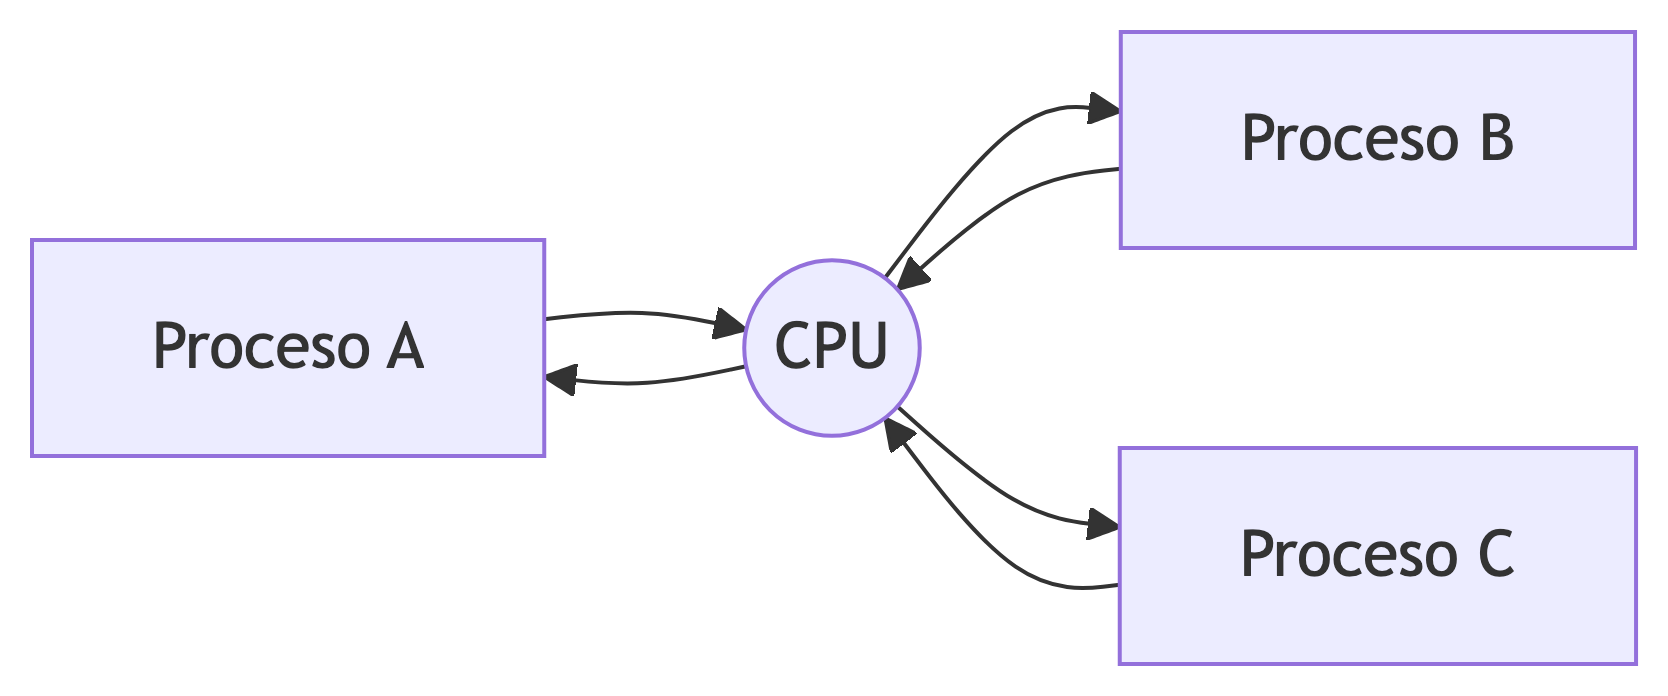
\includegraphics[width=4.34in,height=1.81in]{capitulos/04_administracion_procesos_files/figure-latex/mermaid-figure-1.png}

\begin{tcolorbox}[enhanced jigsaw, arc=.35mm, bottomrule=.15mm, bottomtitle=1mm, breakable, colback=white, colbacktitle=quarto-callout-note-color!10!white, colframe=quarto-callout-note-color-frame, coltitle=black, left=2mm, leftrule=.75mm, opacityback=0, opacitybacktitle=0.6, rightrule=.15mm, title=\textcolor{quarto-callout-note-color}{\faInfo}\hspace{0.5em}{Idea clave}, titlerule=0mm, toprule=.15mm, toptitle=1mm]

La multitarea es posible porque el Sistema Operativo cambia rápidamente
entre procesos mediante el \textbf{Cambio de Contexto (Context Switch)}.

\end{tcolorbox}

\bookmarksetup{startatroot}

\chapter{Programa vs.~Proceso}\label{programa-vs.-proceso}

Un único programa puede generar múltiples procesos independientes.

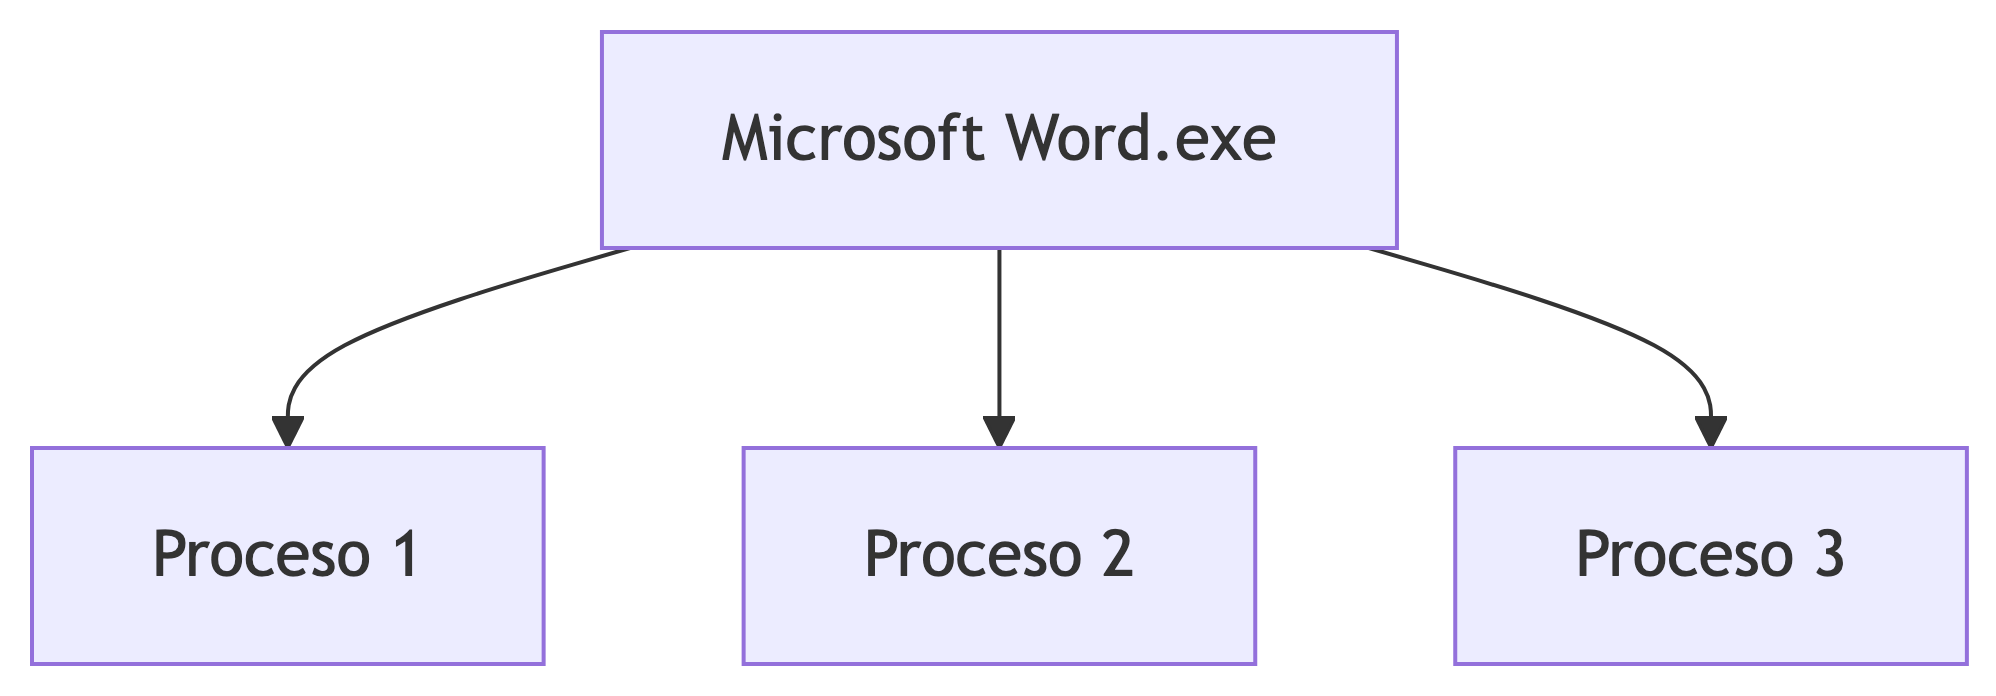
\includegraphics[width=5.21in,height=1.81in]{capitulos/04_administracion_procesos_files/figure-latex/mermaid-figure-10.png}

\bookmarksetup{startatroot}

\chapter{Espacio de Direcciones}\label{espacio-de-direcciones}

Cada proceso dispone de un espacio de memoria independiente.

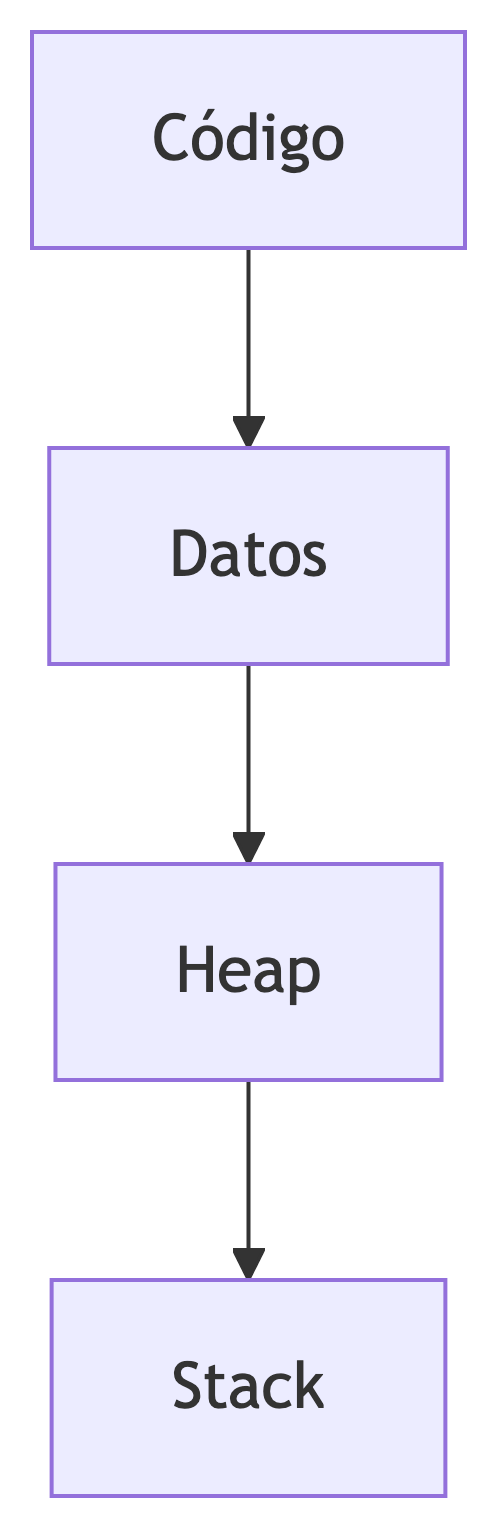
\includegraphics[width=1.29in,height=3.98in]{capitulos/04_administracion_procesos_files/figure-latex/mermaid-figure-9.png}

\bookmarksetup{startatroot}

\chapter{Bloque de Control del Proceso
(PCB)}\label{bloque-de-control-del-proceso-pcb}

El PCB es el expediente administrativo del proceso.

{\def\LTcaptype{none} % do not increment counter
\begin{longtable}[]{@{}ll@{}}
\toprule\noalign{}
Campo & Descripción \\
\midrule\noalign{}
\endhead
\bottomrule\noalign{}
\endlastfoot
PID & Identificador único \\
Estado & Estado actual \\
Program Counter & Próxima instrucción \\
Registros & Contexto de CPU \\
Memoria & Espacio asignado \\
Archivos & Recursos abiertos \\
\end{longtable}
}

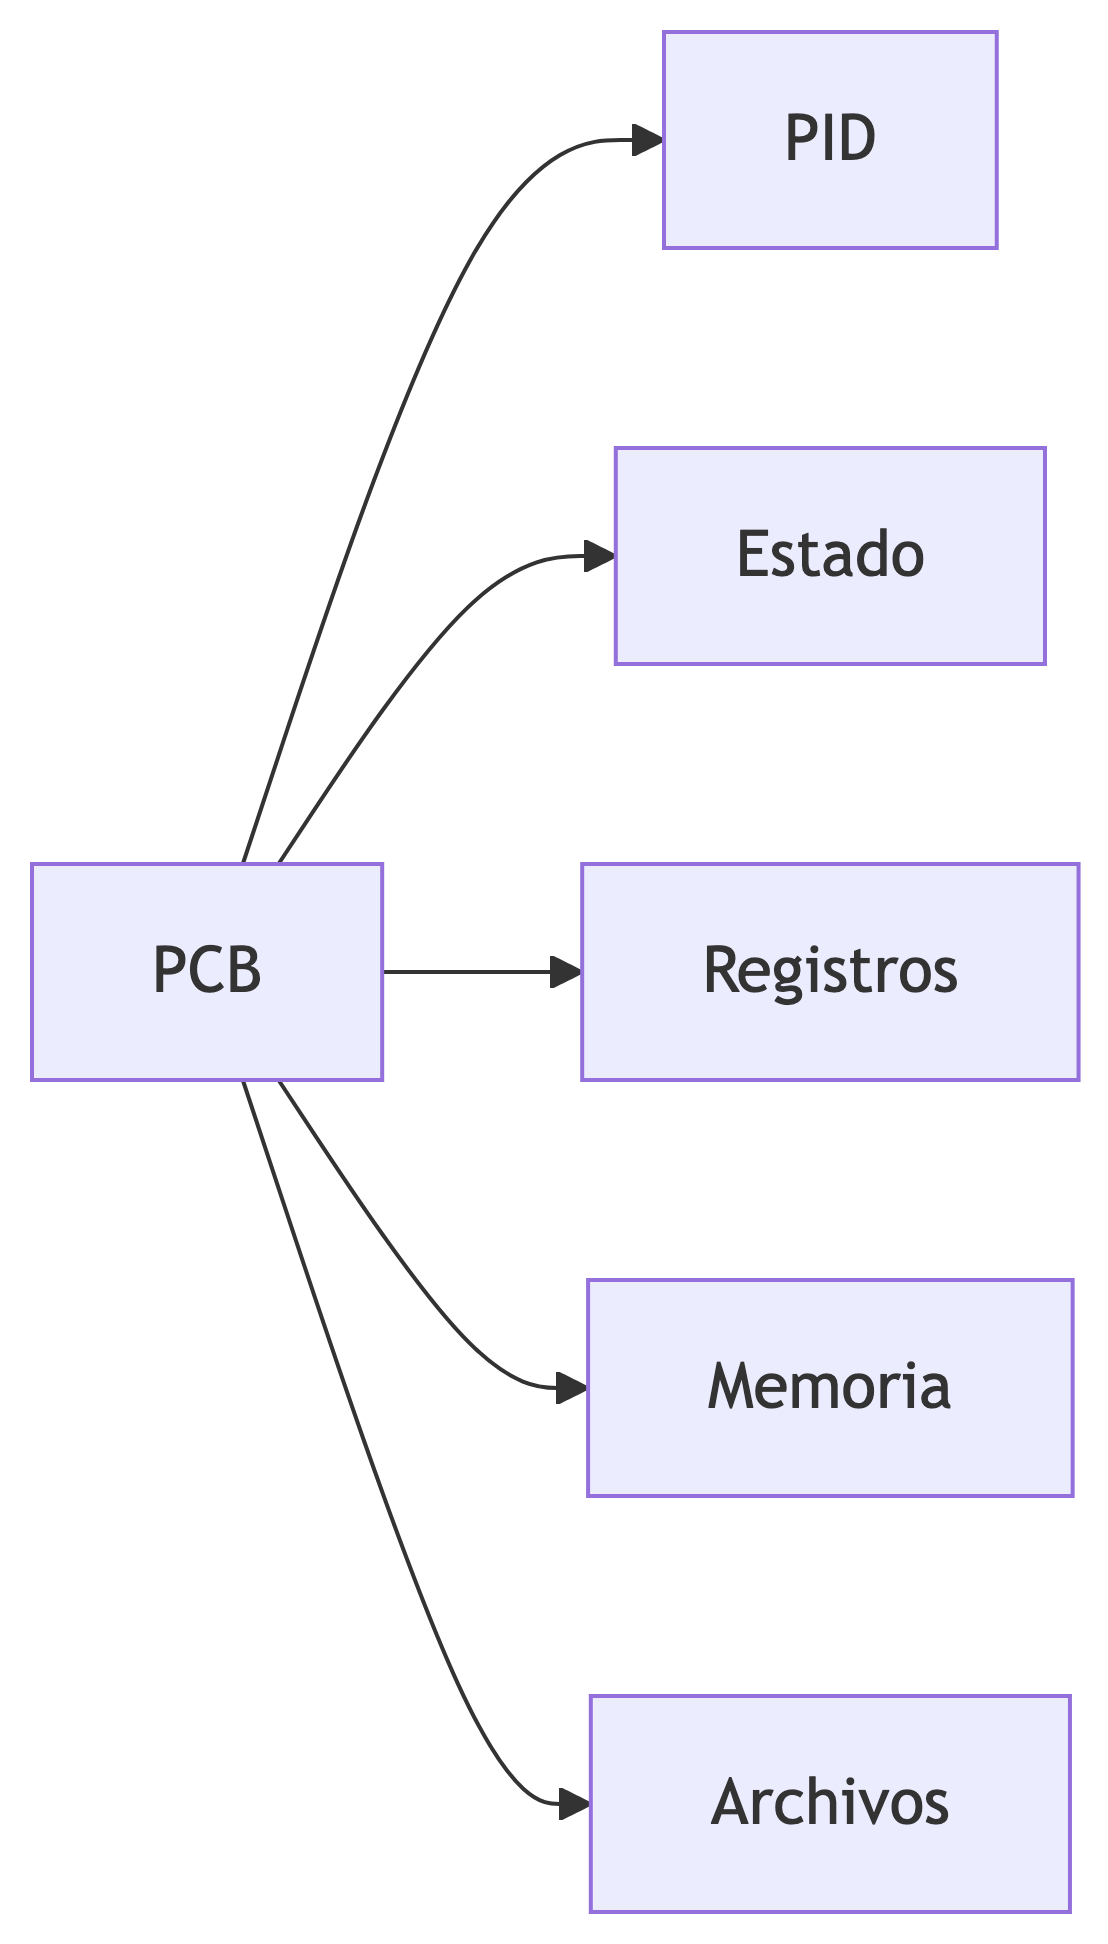
\includegraphics[width=2.89in,height=5.06in]{capitulos/04_administracion_procesos_files/figure-latex/mermaid-figure-8.png}

\bookmarksetup{startatroot}

\chapter{Tabla de Procesos}\label{tabla-de-procesos}

El kernel mantiene una tabla donde registra todos los PCB existentes.

\begin{tcolorbox}[enhanced jigsaw, arc=.35mm, bottomrule=.15mm, bottomtitle=1mm, breakable, colback=white, colbacktitle=quarto-callout-tip-color!10!white, colframe=quarto-callout-tip-color-frame, coltitle=black, left=2mm, leftrule=.75mm, opacityback=0, opacitybacktitle=0.6, rightrule=.15mm, title=\textcolor{quarto-callout-tip-color}{\faLightbulb}\hspace{0.5em}{Estructura simplificada de una Tabla de Procesos}, titlerule=0mm, toprule=.15mm, toptitle=1mm]

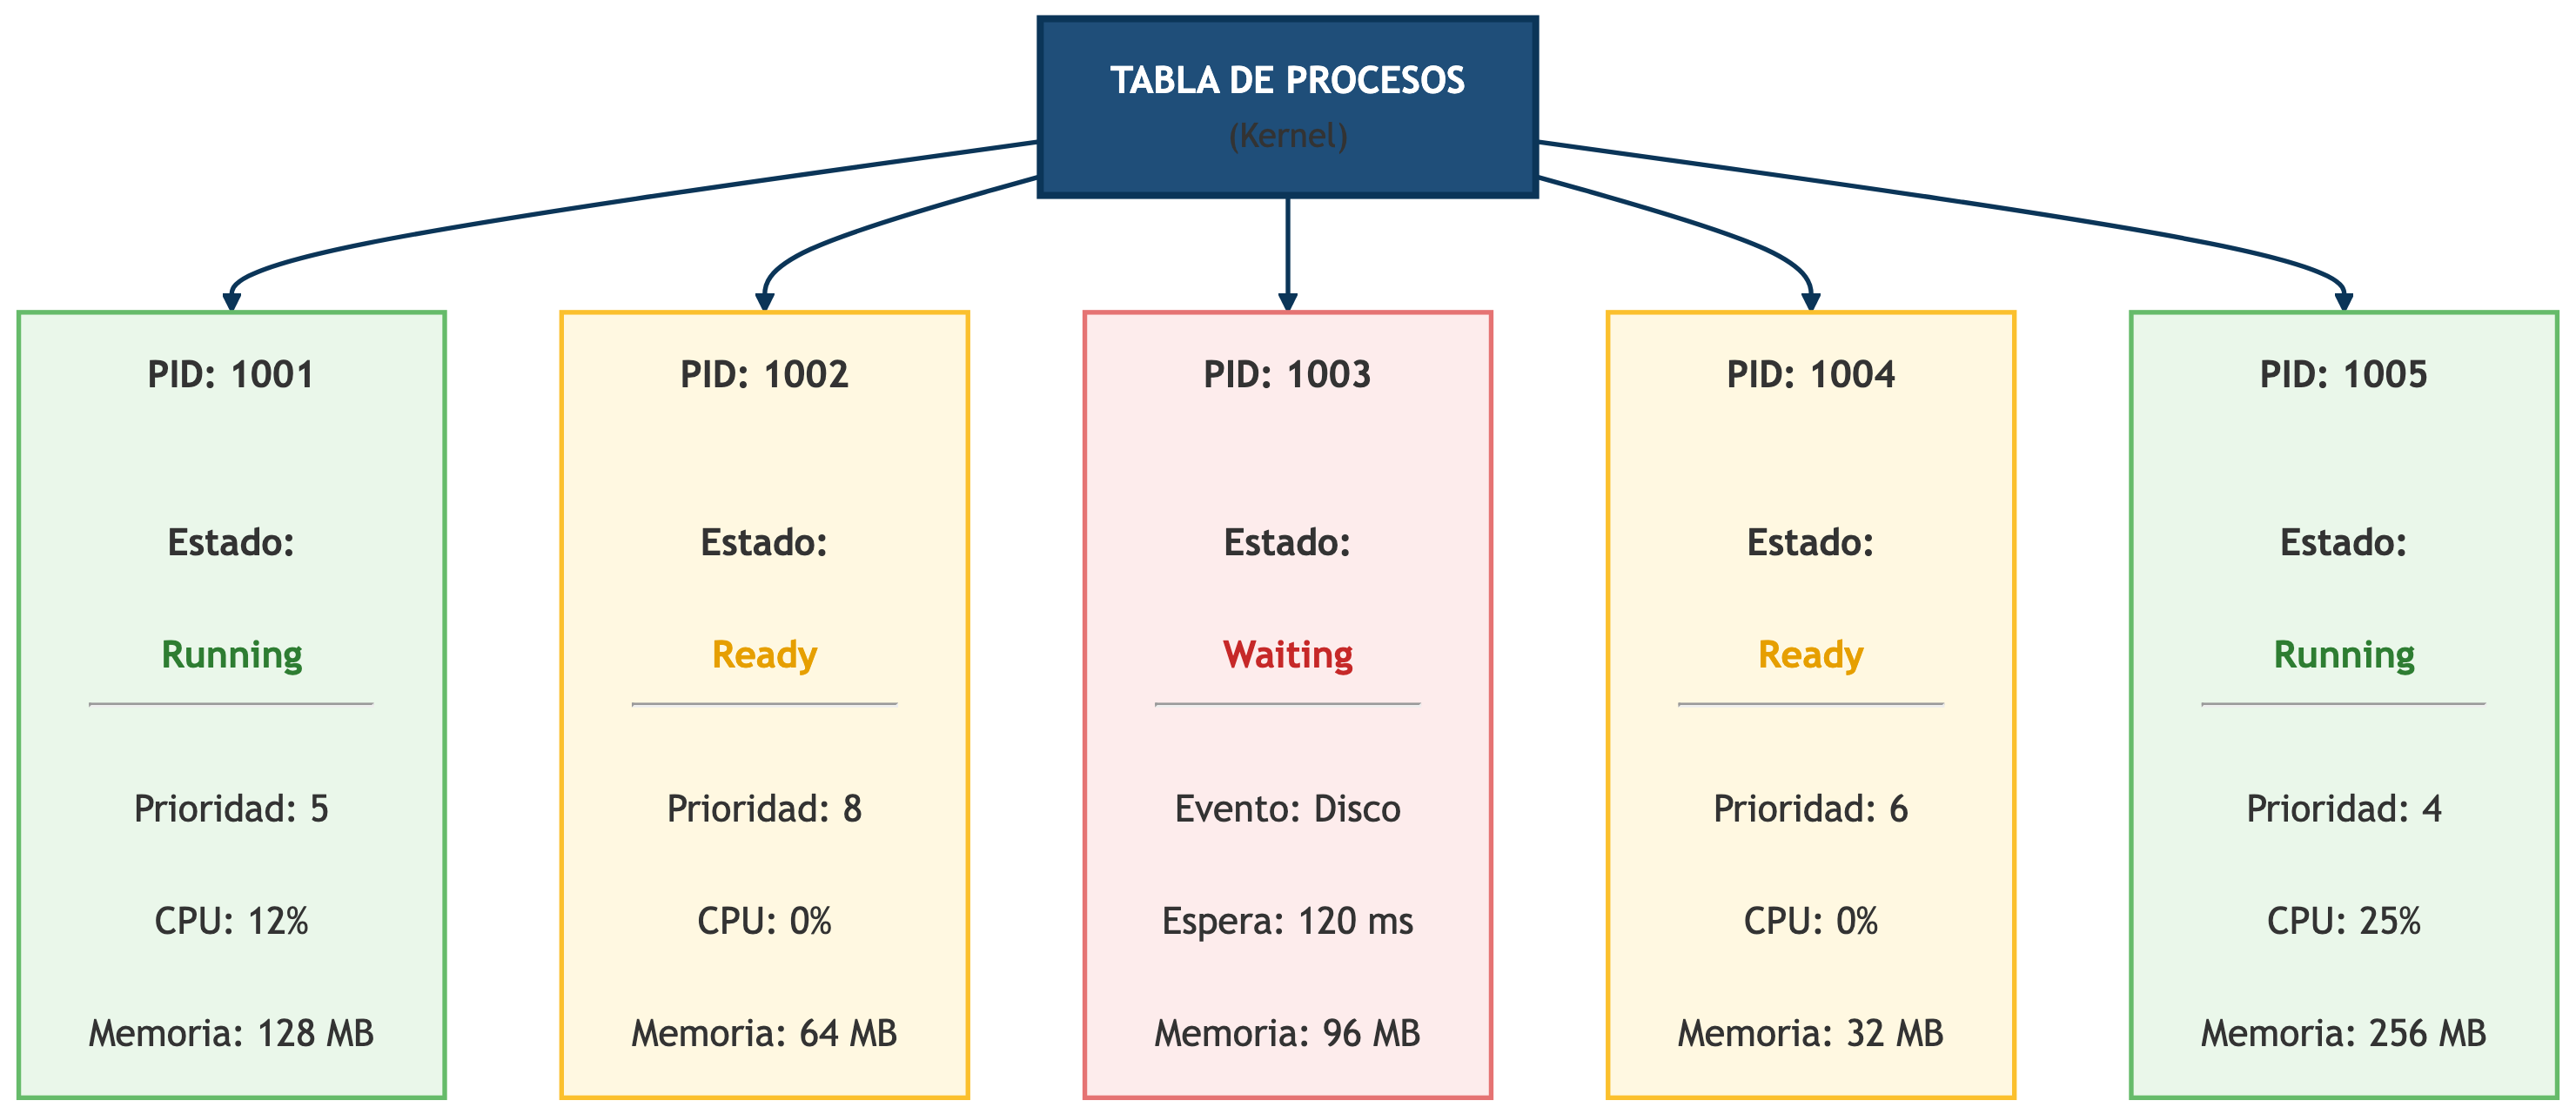
\includegraphics[width=11.01in,height=2.31in]{capitulos/04_administracion_procesos_files/figure-latex/mermaid-figure-7.png}

La tabla de procesos es una estructura interna mantenida por el
\textbf{Kernel}, donde se almacena el \textbf{PCB (Process Control
Block)} de todos los procesos existentes en el sistema. Cada entrada
contiene la información necesaria para que el sistema operativo pueda
administrar correctamente cada proceso.

\end{tcolorbox}

\subsection{Ejemplo de una Tabla de
Procesos}\label{ejemplo-de-una-tabla-de-procesos}

{\def\LTcaptype{none} % do not increment counter
\begin{longtable}[]{@{}
  >{\centering\arraybackslash}p{(\linewidth - 12\tabcolsep) * \real{0.0575}}
  >{\raggedright\arraybackslash}p{(\linewidth - 12\tabcolsep) * \real{0.2299}}
  >{\centering\arraybackslash}p{(\linewidth - 12\tabcolsep) * \real{0.1034}}
  >{\centering\arraybackslash}p{(\linewidth - 12\tabcolsep) * \real{0.1264}}
  >{\raggedleft\arraybackslash}p{(\linewidth - 12\tabcolsep) * \real{0.1609}}
  >{\raggedleft\arraybackslash}p{(\linewidth - 12\tabcolsep) * \real{0.1034}}
  >{\raggedleft\arraybackslash}p{(\linewidth - 12\tabcolsep) * \real{0.2184}}@{}}
\toprule\noalign{}
\begin{minipage}[b]{\linewidth}\centering
PID
\end{minipage} & \begin{minipage}[b]{\linewidth}\raggedright
Nombre del proceso
\end{minipage} & \begin{minipage}[b]{\linewidth}\centering
Estado
\end{minipage} & \begin{minipage}[b]{\linewidth}\centering
Prioridad
\end{minipage} & \begin{minipage}[b]{\linewidth}\raggedleft
Memoria (MB)
\end{minipage} & \begin{minipage}[b]{\linewidth}\raggedleft
CPU (\%)
\end{minipage} & \begin{minipage}[b]{\linewidth}\raggedleft
Archivos abiertos
\end{minipage} \\
\midrule\noalign{}
\endhead
\bottomrule\noalign{}
\endlastfoot
1001 & Chrome.exe & Running & Alta & 245 & 18 & 27 \\
1002 & Word.exe & Ready & Media & 132 & 0 & 12 \\
1003 & Spotify.exe & Waiting & Baja & 95 & 0 & 8 \\
1004 & Teams.exe & Ready & Alta & 318 & 0 & 34 \\
1005 & Explorer.exe & Running & Alta & 76 & 5 & 19 \\
\end{longtable}
}

\textbf{Interpretación}

\begin{itemize}
\tightlist
\item
  \textbf{PID:} Identificador único asignado por el sistema operativo.
\item
  \textbf{Nombre del proceso:} Aplicación o servicio que se encuentra en
  ejecución.
\item
  \textbf{Estado:} Situación actual del proceso (Running, Ready o
  Waiting).
\item
  \textbf{Prioridad:} Nivel de importancia utilizado por el Scheduler.
\item
  \textbf{Memoria:} Cantidad de memoria RAM reservada por el proceso.
\item
  \textbf{CPU:} Porcentaje de utilización del procesador en ese
  instante.
\item
  \textbf{Archivos abiertos:} Número de archivos o recursos que el
  proceso mantiene abiertos.
\end{itemize}

\bookmarksetup{startatroot}

\chapter{Módelos de Estados de un
Proceso}\label{muxf3delos-de-estados-de-un-proceso}

\section{Evolución de los modelos de
estados}\label{evoluciuxf3n-de-los-modelos-de-estados}

{\def\LTcaptype{none} % do not increment counter
\begin{longtable}[]{@{}
  >{\raggedright\arraybackslash}p{(\linewidth - 4\tabcolsep) * \real{0.2368}}
  >{\raggedright\arraybackslash}p{(\linewidth - 4\tabcolsep) * \real{0.2368}}
  >{\raggedright\arraybackslash}p{(\linewidth - 4\tabcolsep) * \real{0.5263}}@{}}
\toprule\noalign{}
\begin{minipage}[b]{\linewidth}\raggedright
Modelo
\end{minipage} & \begin{minipage}[b]{\linewidth}\raggedright
Estados
\end{minipage} & \begin{minipage}[b]{\linewidth}\raggedright
¿Dónde se utiliza?
\end{minipage} \\
\midrule\noalign{}
\endhead
\bottomrule\noalign{}
\endlastfoot
Dos estados & Listo y Ejecución & Sistemas muy simples o con fines
didácticos. \\
Cinco estados & Nuevo, Listo, Ejecución, Bloqueado y Terminado & Es el
modelo más utilizado para explicar la administración de procesos. \\
Siete estados & Cinco estados + Listo Suspendido + Bloqueado Suspendido
& Sistemas operativos modernos que utilizan memoria virtual y Swap. \\
\end{longtable}
}

\section{Modelo de cinco estados}\label{modelo-de-cinco-estados}

El modelo de cinco estados es uno de los más utilizados para explicar el
ciclo de vida de un proceso en un sistema operativo. En este modelo, un
proceso puede encontrarse en uno de cinco estados bien definidos, y el
sistema operativo controla las transiciones entre ellos.

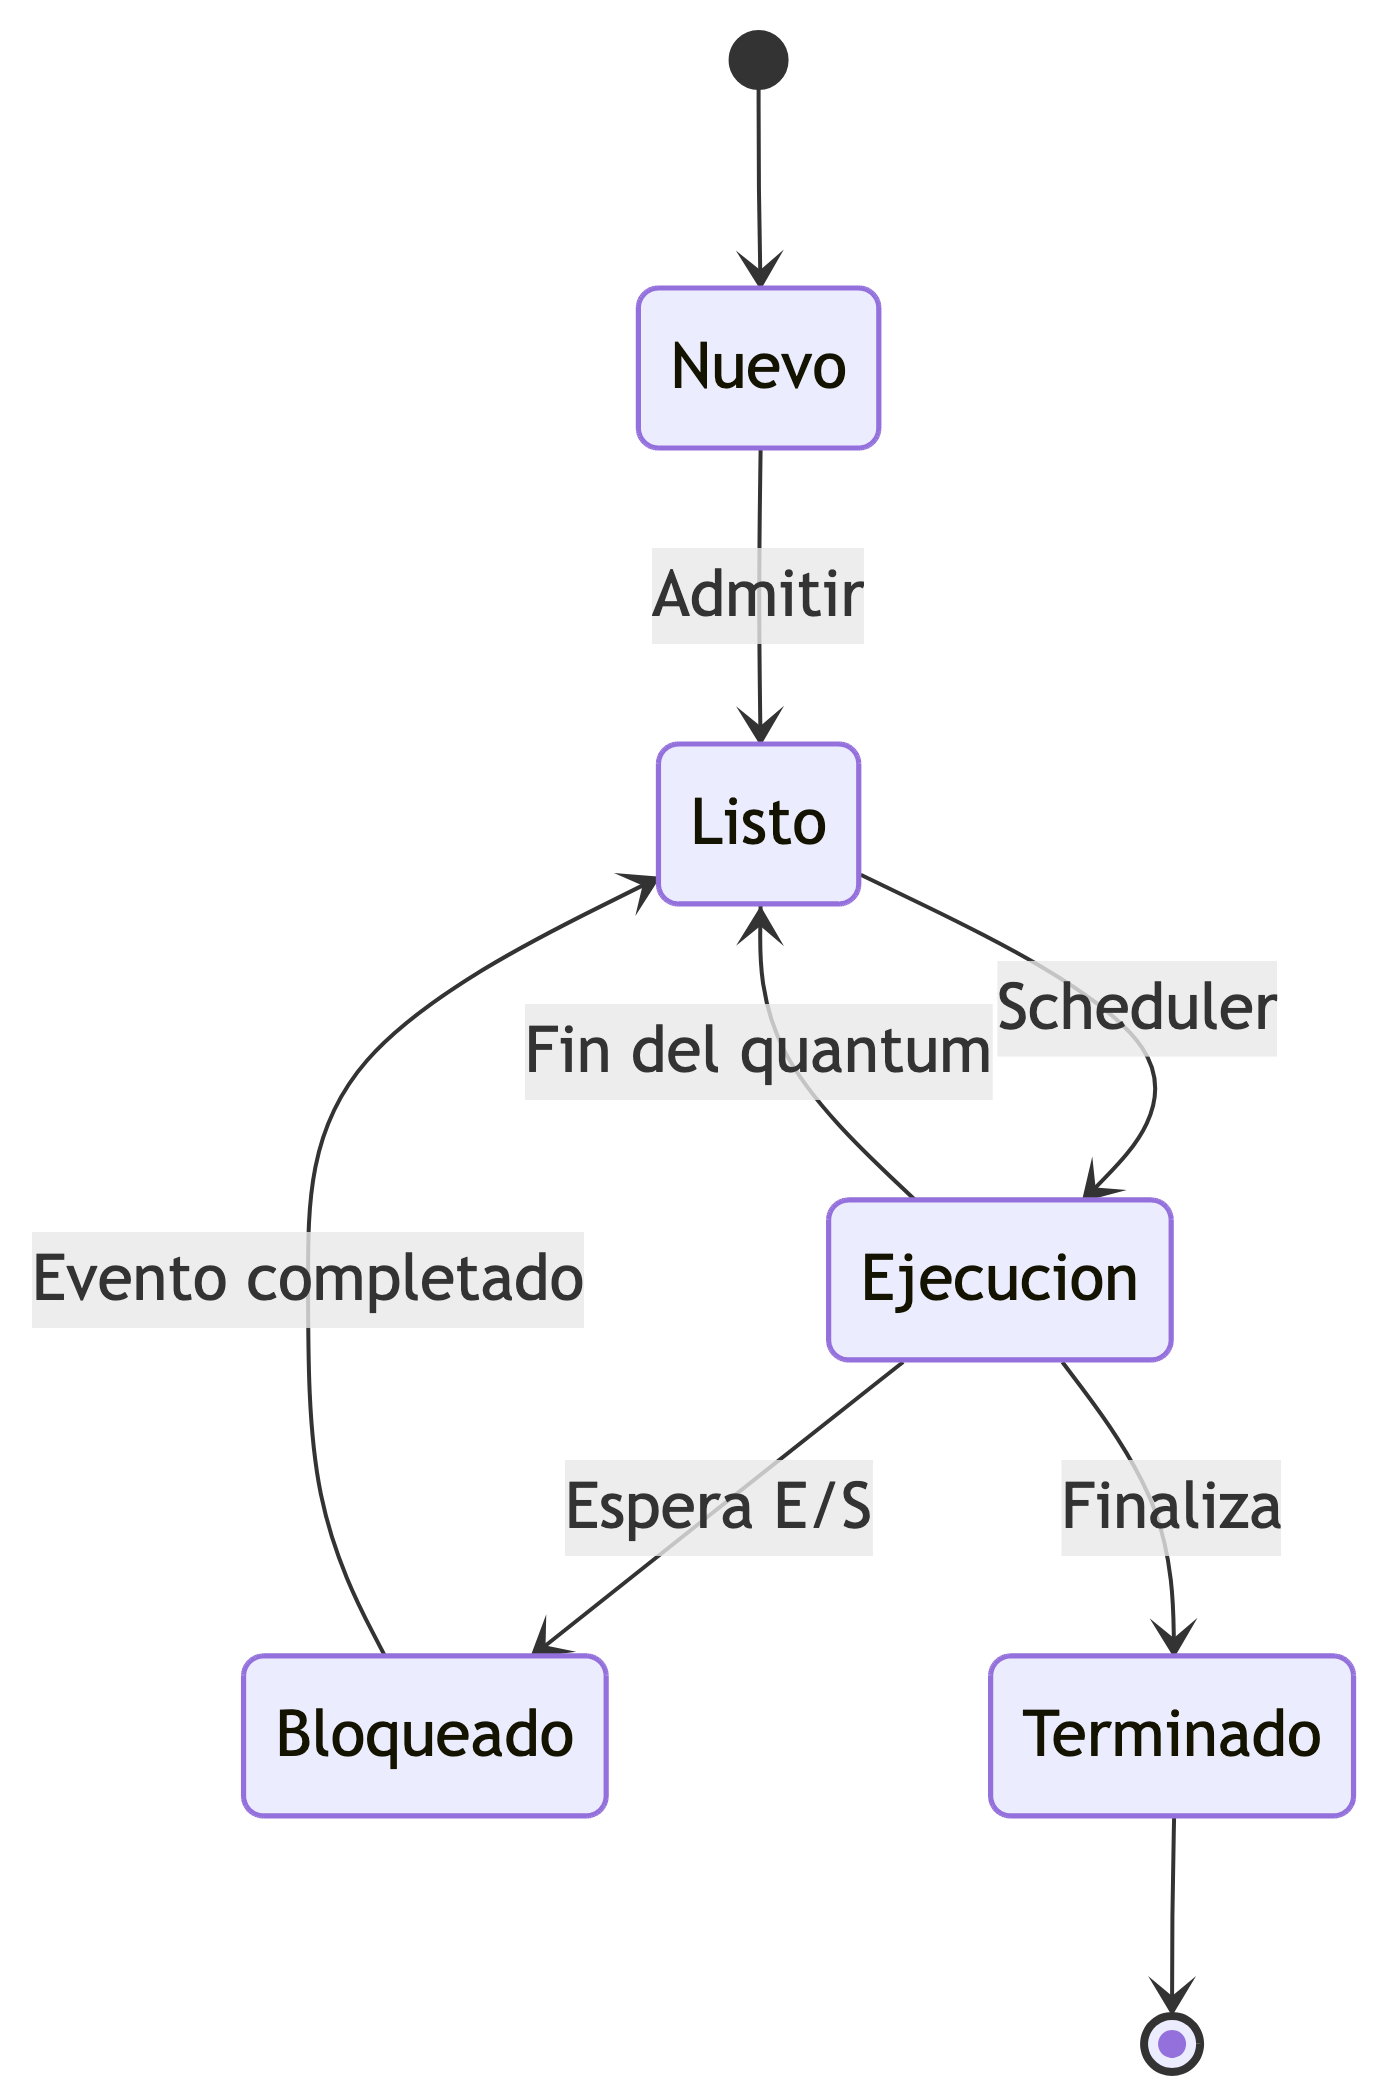
\includegraphics[width=3.61in,height=5.48in]{capitulos/04_administracion_procesos_files/figure-latex/mermaid-figure-6.png}

\subsection{Descripción de los
estados}\label{descripciuxf3n-de-los-estados}

{\def\LTcaptype{none} % do not increment counter
\begin{longtable}[]{@{}
  >{\raggedright\arraybackslash}p{(\linewidth - 2\tabcolsep) * \real{0.4091}}
  >{\raggedright\arraybackslash}p{(\linewidth - 2\tabcolsep) * \real{0.5909}}@{}}
\toprule\noalign{}
\begin{minipage}[b]{\linewidth}\raggedright
Estado
\end{minipage} & \begin{minipage}[b]{\linewidth}\raggedright
Descripción
\end{minipage} \\
\midrule\noalign{}
\endhead
\bottomrule\noalign{}
\endlastfoot
\textbf{Nuevo} & El proceso acaba de ser creado y aún no está listo para
ejecutarse. \\
\textbf{Listo (Ready)} & El proceso posee todos los recursos necesarios
excepto la CPU. Espera su turno para ejecutarse. \\
\textbf{Ejecución (Running)} & El proceso está utilizando el procesador
y ejecutando instrucciones. \\
\textbf{Bloqueado (Waiting)} & El proceso espera la finalización de una
operación de entrada/salida o algún evento externo. \\
\textbf{Terminado (Exit)} & El proceso concluyó su ejecución y el
sistema operativo libera los recursos utilizados. \\
\end{longtable}
}

\begin{tcolorbox}[enhanced jigsaw, arc=.35mm, bottomrule=.15mm, bottomtitle=1mm, breakable, colback=white, colbacktitle=quarto-callout-tip-color!10!white, colframe=quarto-callout-tip-color-frame, coltitle=black, left=2mm, leftrule=.75mm, opacityback=0, opacitybacktitle=0.6, rightrule=.15mm, title=\textcolor{quarto-callout-tip-color}{\faLightbulb}\hspace{0.5em}{Idea clave}, titlerule=0mm, toprule=.15mm, toptitle=1mm]

Todo proceso pasa necesariamente por los estados \textbf{Nuevo} y
\textbf{Terminado}, mientras que los estados \textbf{Listo},
\textbf{Ejecución} y \textbf{Bloqueado} pueden repetirse varias veces
durante su ciclo de vida.

\end{tcolorbox}

\section{Modelo con procesos suspendidos
(Swap)}\label{modelo-con-procesos-suspendidos-swap}

En sistemas multitarea es posible que la memoria principal no sea
suficiente para mantener todos los procesos cargados simultáneamente. En
estos casos, el sistema operativo puede mover temporalmente algunos
procesos al almacenamiento secundario mediante una técnica denominada
\textbf{Swap} o \textbf{Intercambio de memoria}.

Cuando esto ocurre aparecen dos nuevos estados:

\begin{itemize}
\tightlist
\item
  \textbf{Listo y Suspendido}
\item
  \textbf{Bloqueado y Suspendido}
\end{itemize}

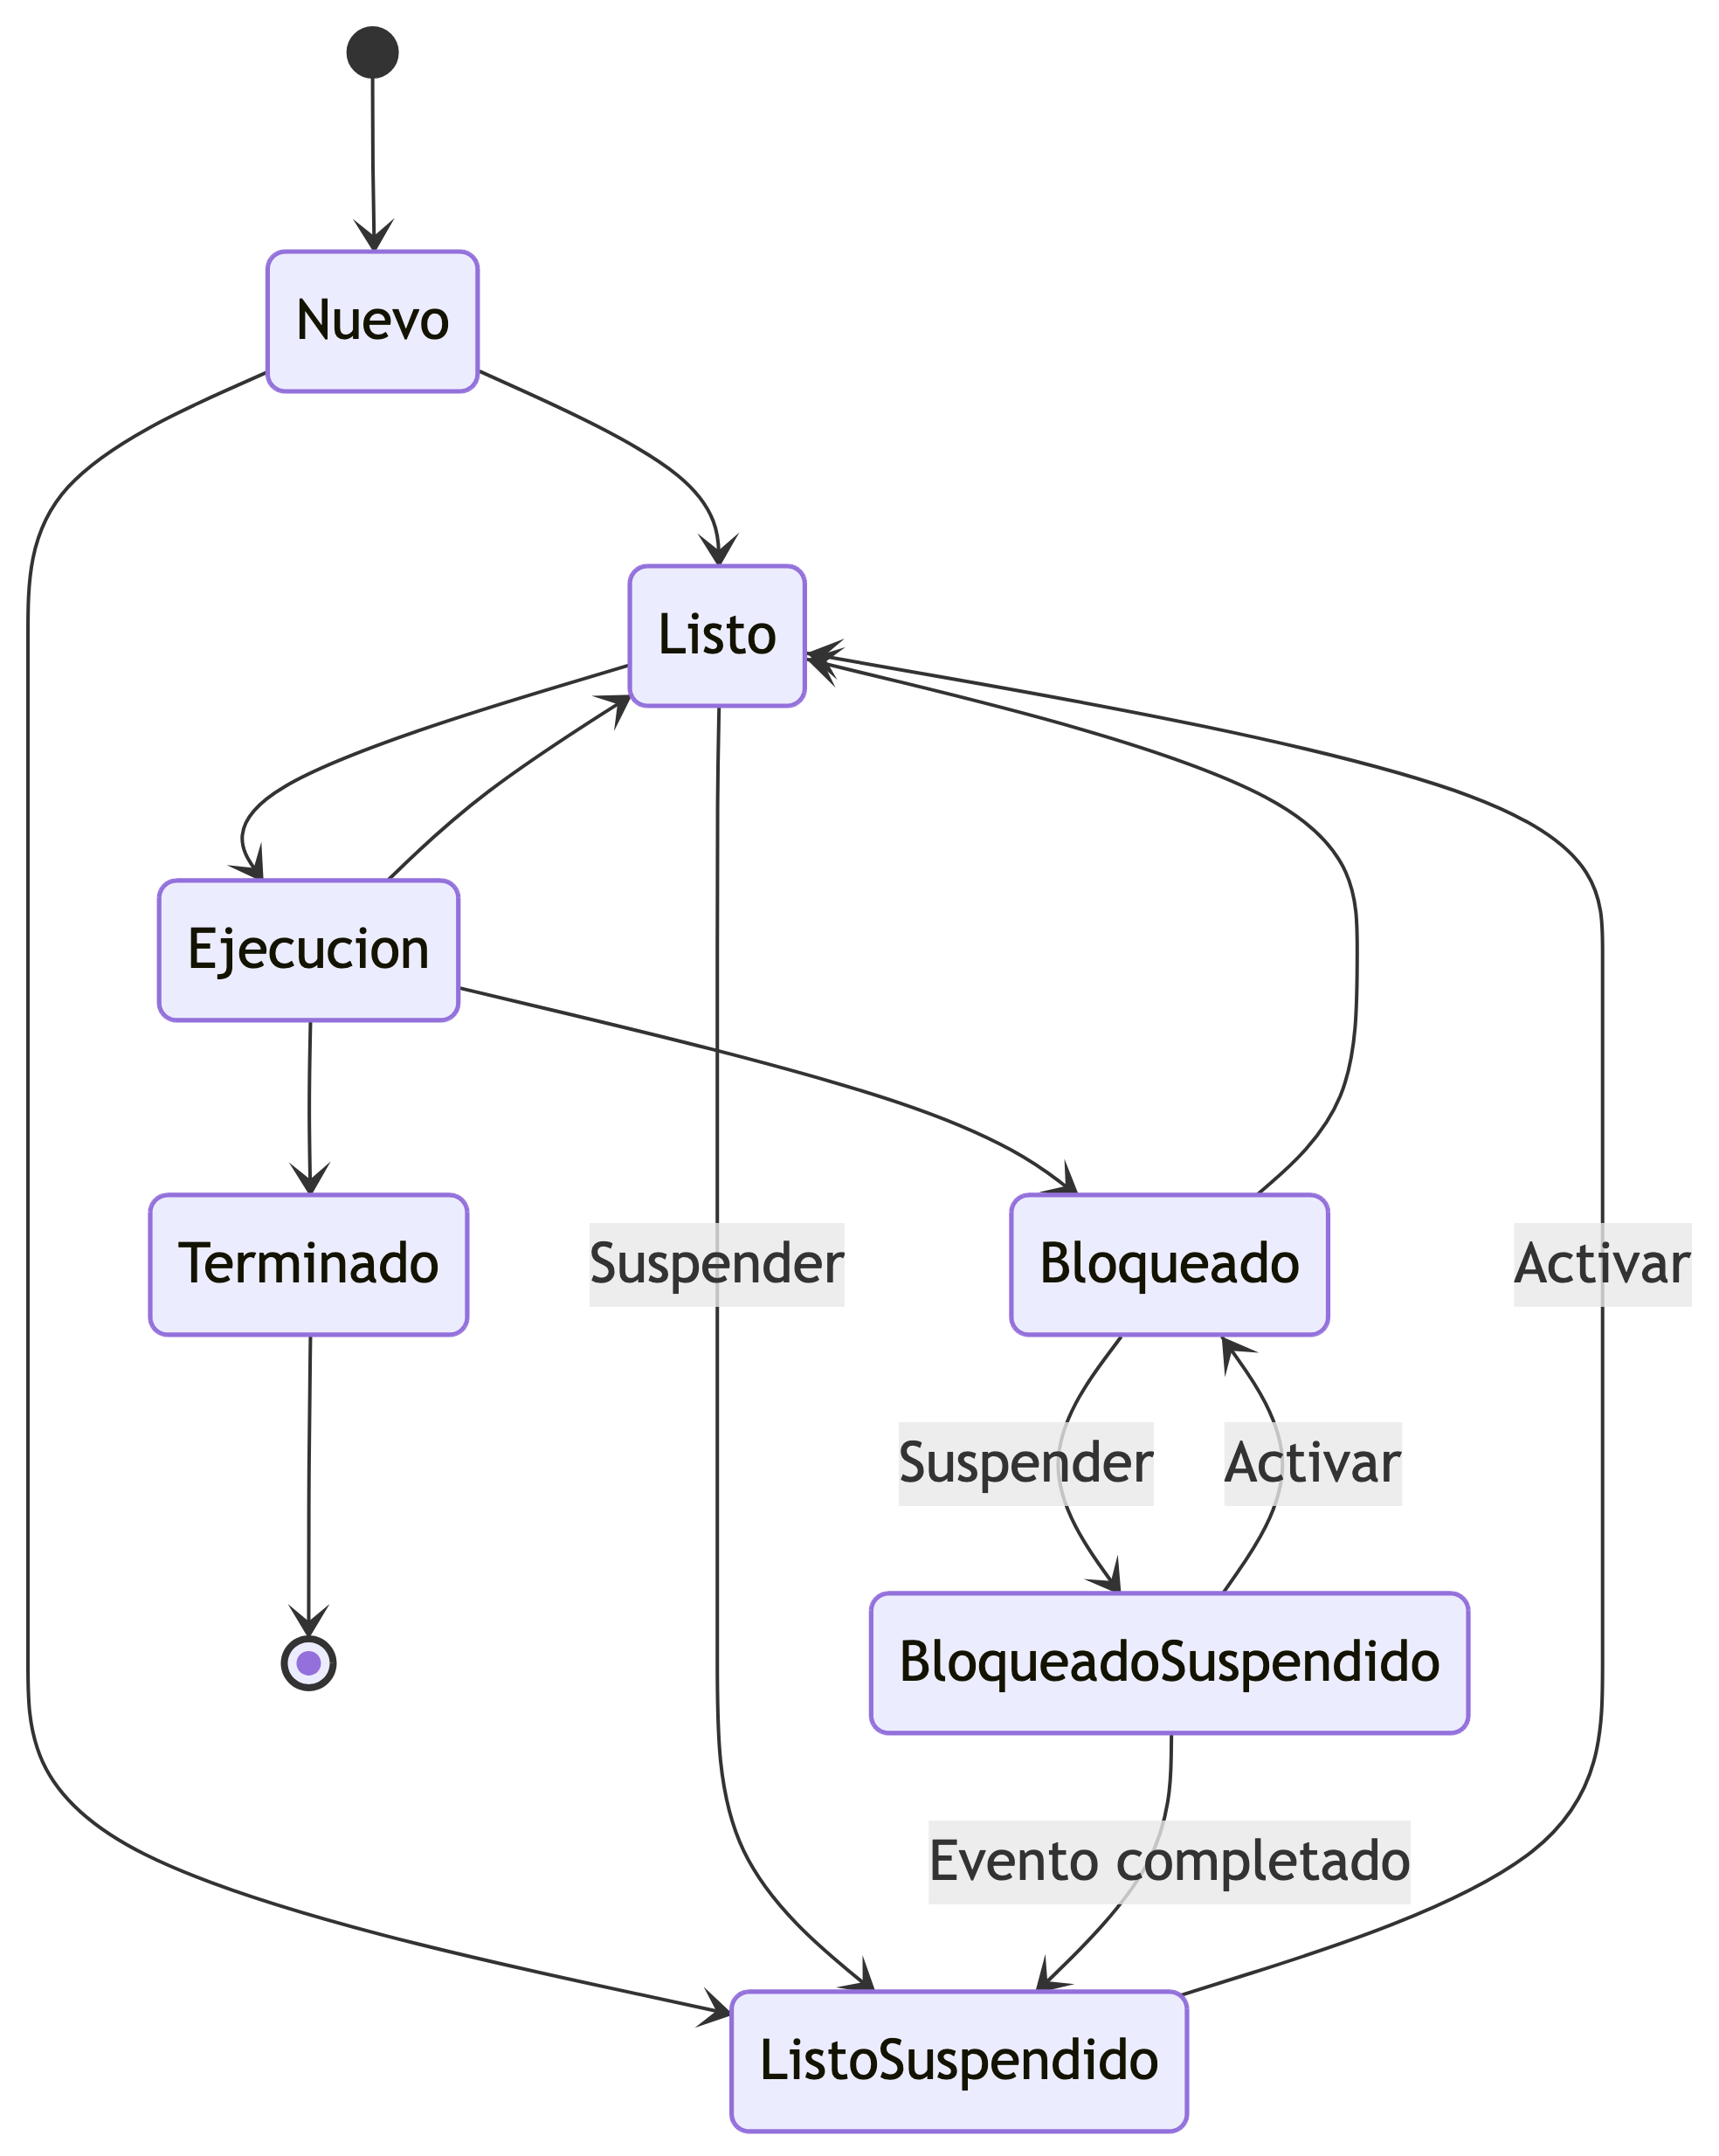
\includegraphics[width=5.13in,height=6.44in]{capitulos/04_administracion_procesos_files/figure-latex/mermaid-figure-5.png}

\subsection{Nuevos estados}\label{nuevos-estados}

{\def\LTcaptype{none} % do not increment counter
\begin{longtable}[]{@{}
  >{\raggedright\arraybackslash}p{(\linewidth - 2\tabcolsep) * \real{0.4091}}
  >{\raggedright\arraybackslash}p{(\linewidth - 2\tabcolsep) * \real{0.5909}}@{}}
\toprule\noalign{}
\begin{minipage}[b]{\linewidth}\raggedright
Estado
\end{minipage} & \begin{minipage}[b]{\linewidth}\raggedright
Descripción
\end{minipage} \\
\midrule\noalign{}
\endhead
\bottomrule\noalign{}
\endlastfoot
\textbf{Listo y Suspendido} & El proceso está preparado para ejecutarse,
pero fue trasladado al disco porque no existe memoria RAM suficiente. \\
\textbf{Bloqueado y Suspendido} & El proceso permanece esperando un
evento y, además, fue movido temporalmente al almacenamiento
secundario. \\
\end{longtable}
}

\begin{tcolorbox}[enhanced jigsaw, arc=.35mm, bottomrule=.15mm, bottomtitle=1mm, breakable, colback=white, colbacktitle=quarto-callout-note-color!10!white, colframe=quarto-callout-note-color-frame, coltitle=black, left=2mm, leftrule=.75mm, opacityback=0, opacitybacktitle=0.6, rightrule=.15mm, title=\textcolor{quarto-callout-note-color}{\faInfo}\hspace{0.5em}{¿Qué es el Swap?}, titlerule=0mm, toprule=.15mm, toptitle=1mm]

El \textbf{Swap} consiste en mover procesos completos o parte de su
memoria desde la RAM hacia un área especial del disco duro o del SSD
para liberar memoria física y permitir que otros procesos continúen
ejecutándose.

Aunque esta técnica incrementa la capacidad de ejecución del sistema,
también reduce el rendimiento, ya que acceder al disco es mucho más
lento que acceder a la memoria RAM.

\end{tcolorbox}

\bookmarksetup{startatroot}

\chapter{Resumen}\label{resumen}

\begin{itemize}
\tightlist
\item
  Un programa se convierte en proceso al ejecutarse.
\item
  Cada proceso posee memoria y recursos propios.
\item
  El PCB almacena toda la información necesaria para administrarlo.
\item
  El Scheduler comparte el procesador entre todos los procesos.
\item
  En la siguiente sección estudiaremos el ciclo de vida y los estados de
  un proceso.
\end{itemize}

\bookmarksetup{startatroot}

\chapter{Scheduler y Dispatcher}\label{scheduler-y-dispatcher}

El \textbf{Scheduler} decide qué proceso obtendrá el procesador cuando
existen varios procesos listos para ejecutarse. Para tomar esta decisión
puede considerar la prioridad, el tiempo de espera o el algoritmo de
planificación configurado por el sistema operativo.

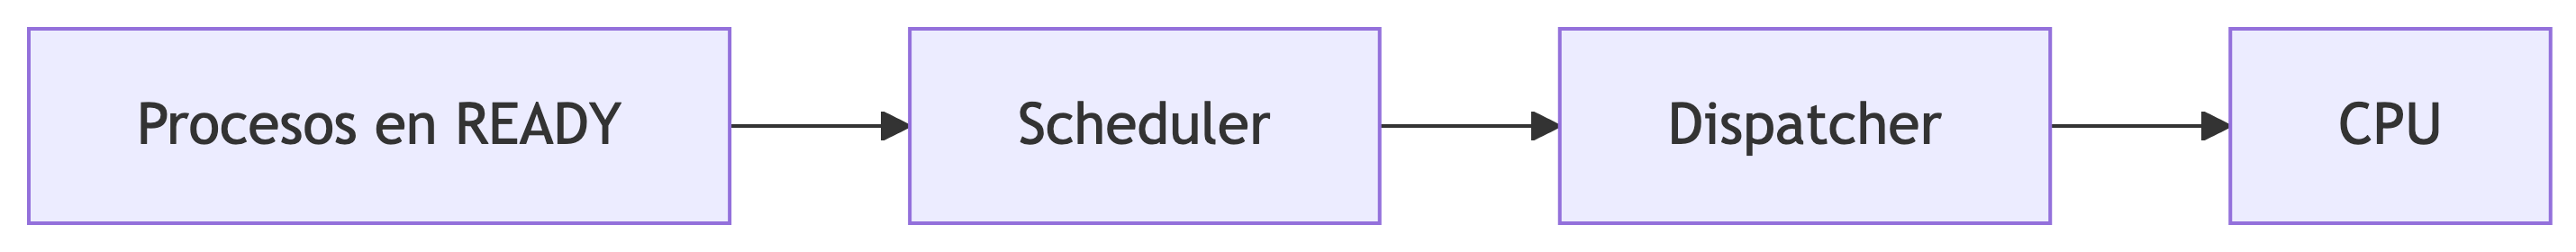
\includegraphics[width=7.46in,height=0.73in]{capitulos/04_administracion_procesos_files/figure-latex/mermaid-figure-4.png}

El \textbf{Dispatcher} es el componente encargado de entregar realmente
la CPU al proceso seleccionado y realizar el cambio de contexto.

\bookmarksetup{startatroot}

\chapter{Cambio de contexto (Context
Switch)}\label{cambio-de-contexto-context-switch}

Un cambio de contexto ocurre cuando el sistema operativo detiene
temporalmente un proceso, guarda su estado en el PCB y restaura el
estado de otro proceso.

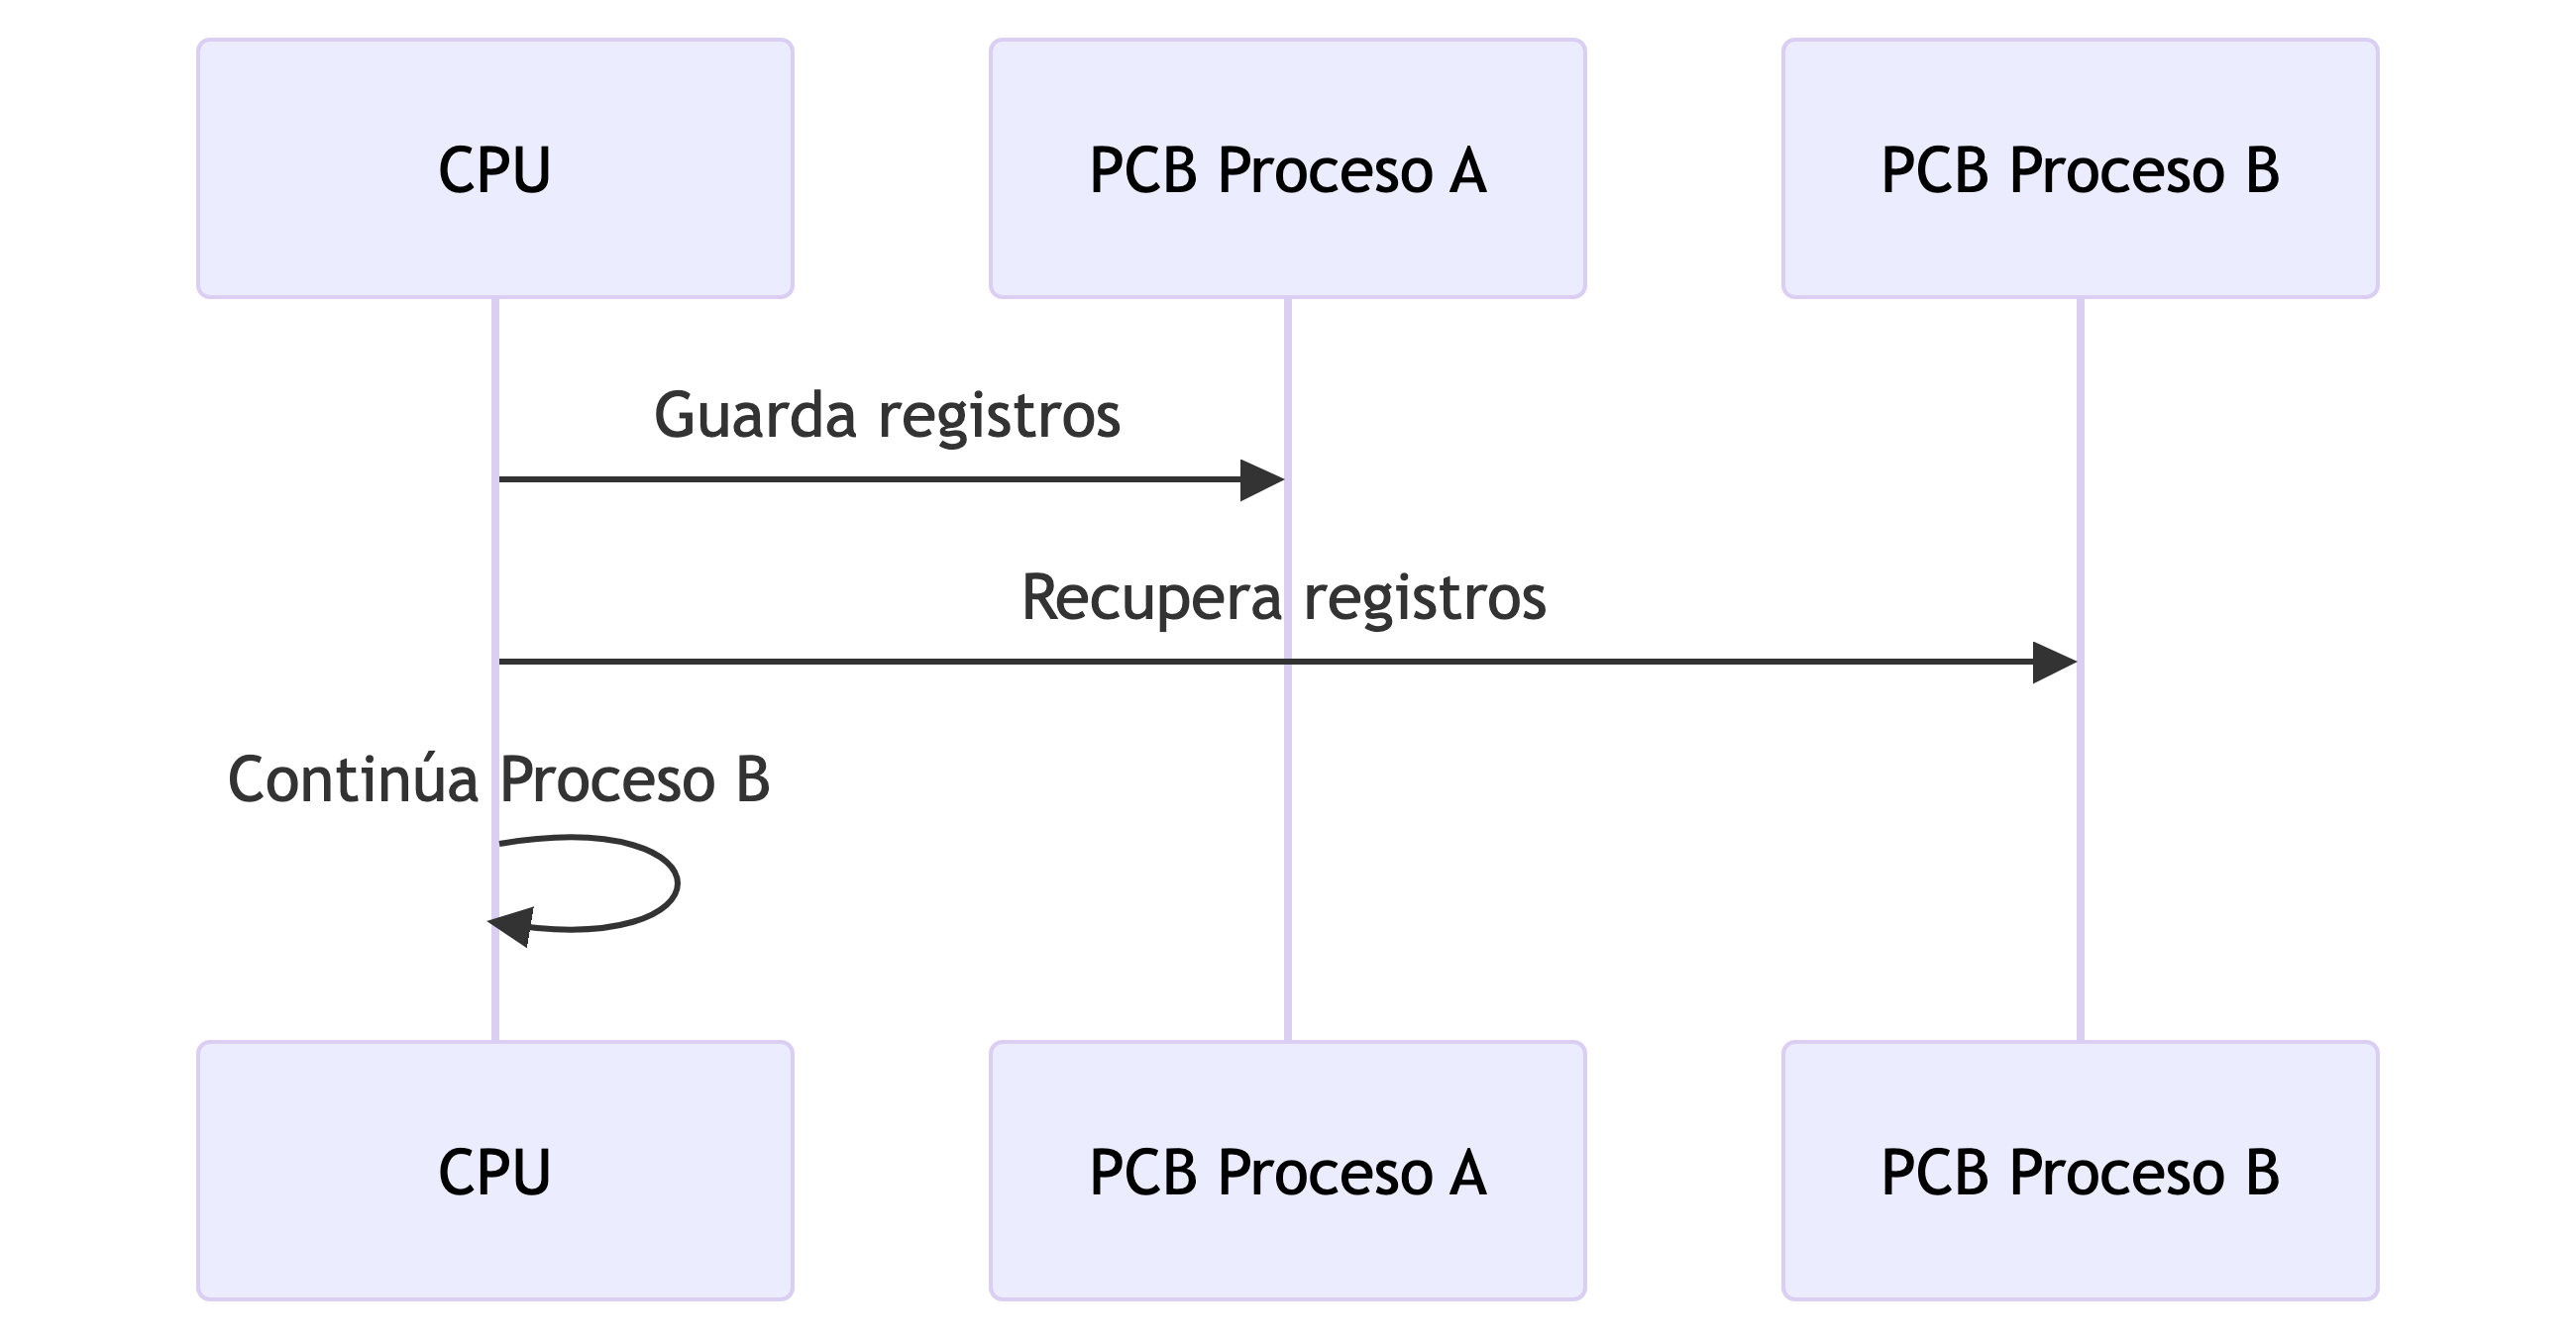
\includegraphics[width=6.77in,height=3.53in]{capitulos/04_administracion_procesos_files/figure-latex/mermaid-figure-3.png}

\bookmarksetup{startatroot}

\chapter{Ejemplo completo: Microsoft
Word}\label{ejemplo-completo-microsoft-word}

\begin{enumerate}
\def\labelenumi{\arabic{enumi}.}
\tightlist
\item
  El usuario hace doble clic sobre \textbf{Word.exe}.
\item
  El Kernel crea el proceso y asigna un PID.
\item
  El proceso entra al estado \textbf{NEW}.
\item
  Se reserva memoria y se crea el PCB.
\item
  El proceso pasa a \textbf{READY}.
\item
  El Scheduler selecciona el proceso.
\item
  El Dispatcher entrega la CPU.
\item
  El proceso entra en \textbf{RUNNING}.
\item
  Al guardar un archivo, espera la respuesta del disco
  (\textbf{WAITING}).
\item
  Finalizada la operación de E/S vuelve a \textbf{READY}.
\item
  El Scheduler le asigna nuevamente la CPU.
\item
  Al cerrar Word, el proceso entra en \textbf{EXIT} y el sistema libera
  memoria, archivos y demás recursos.
\end{enumerate}

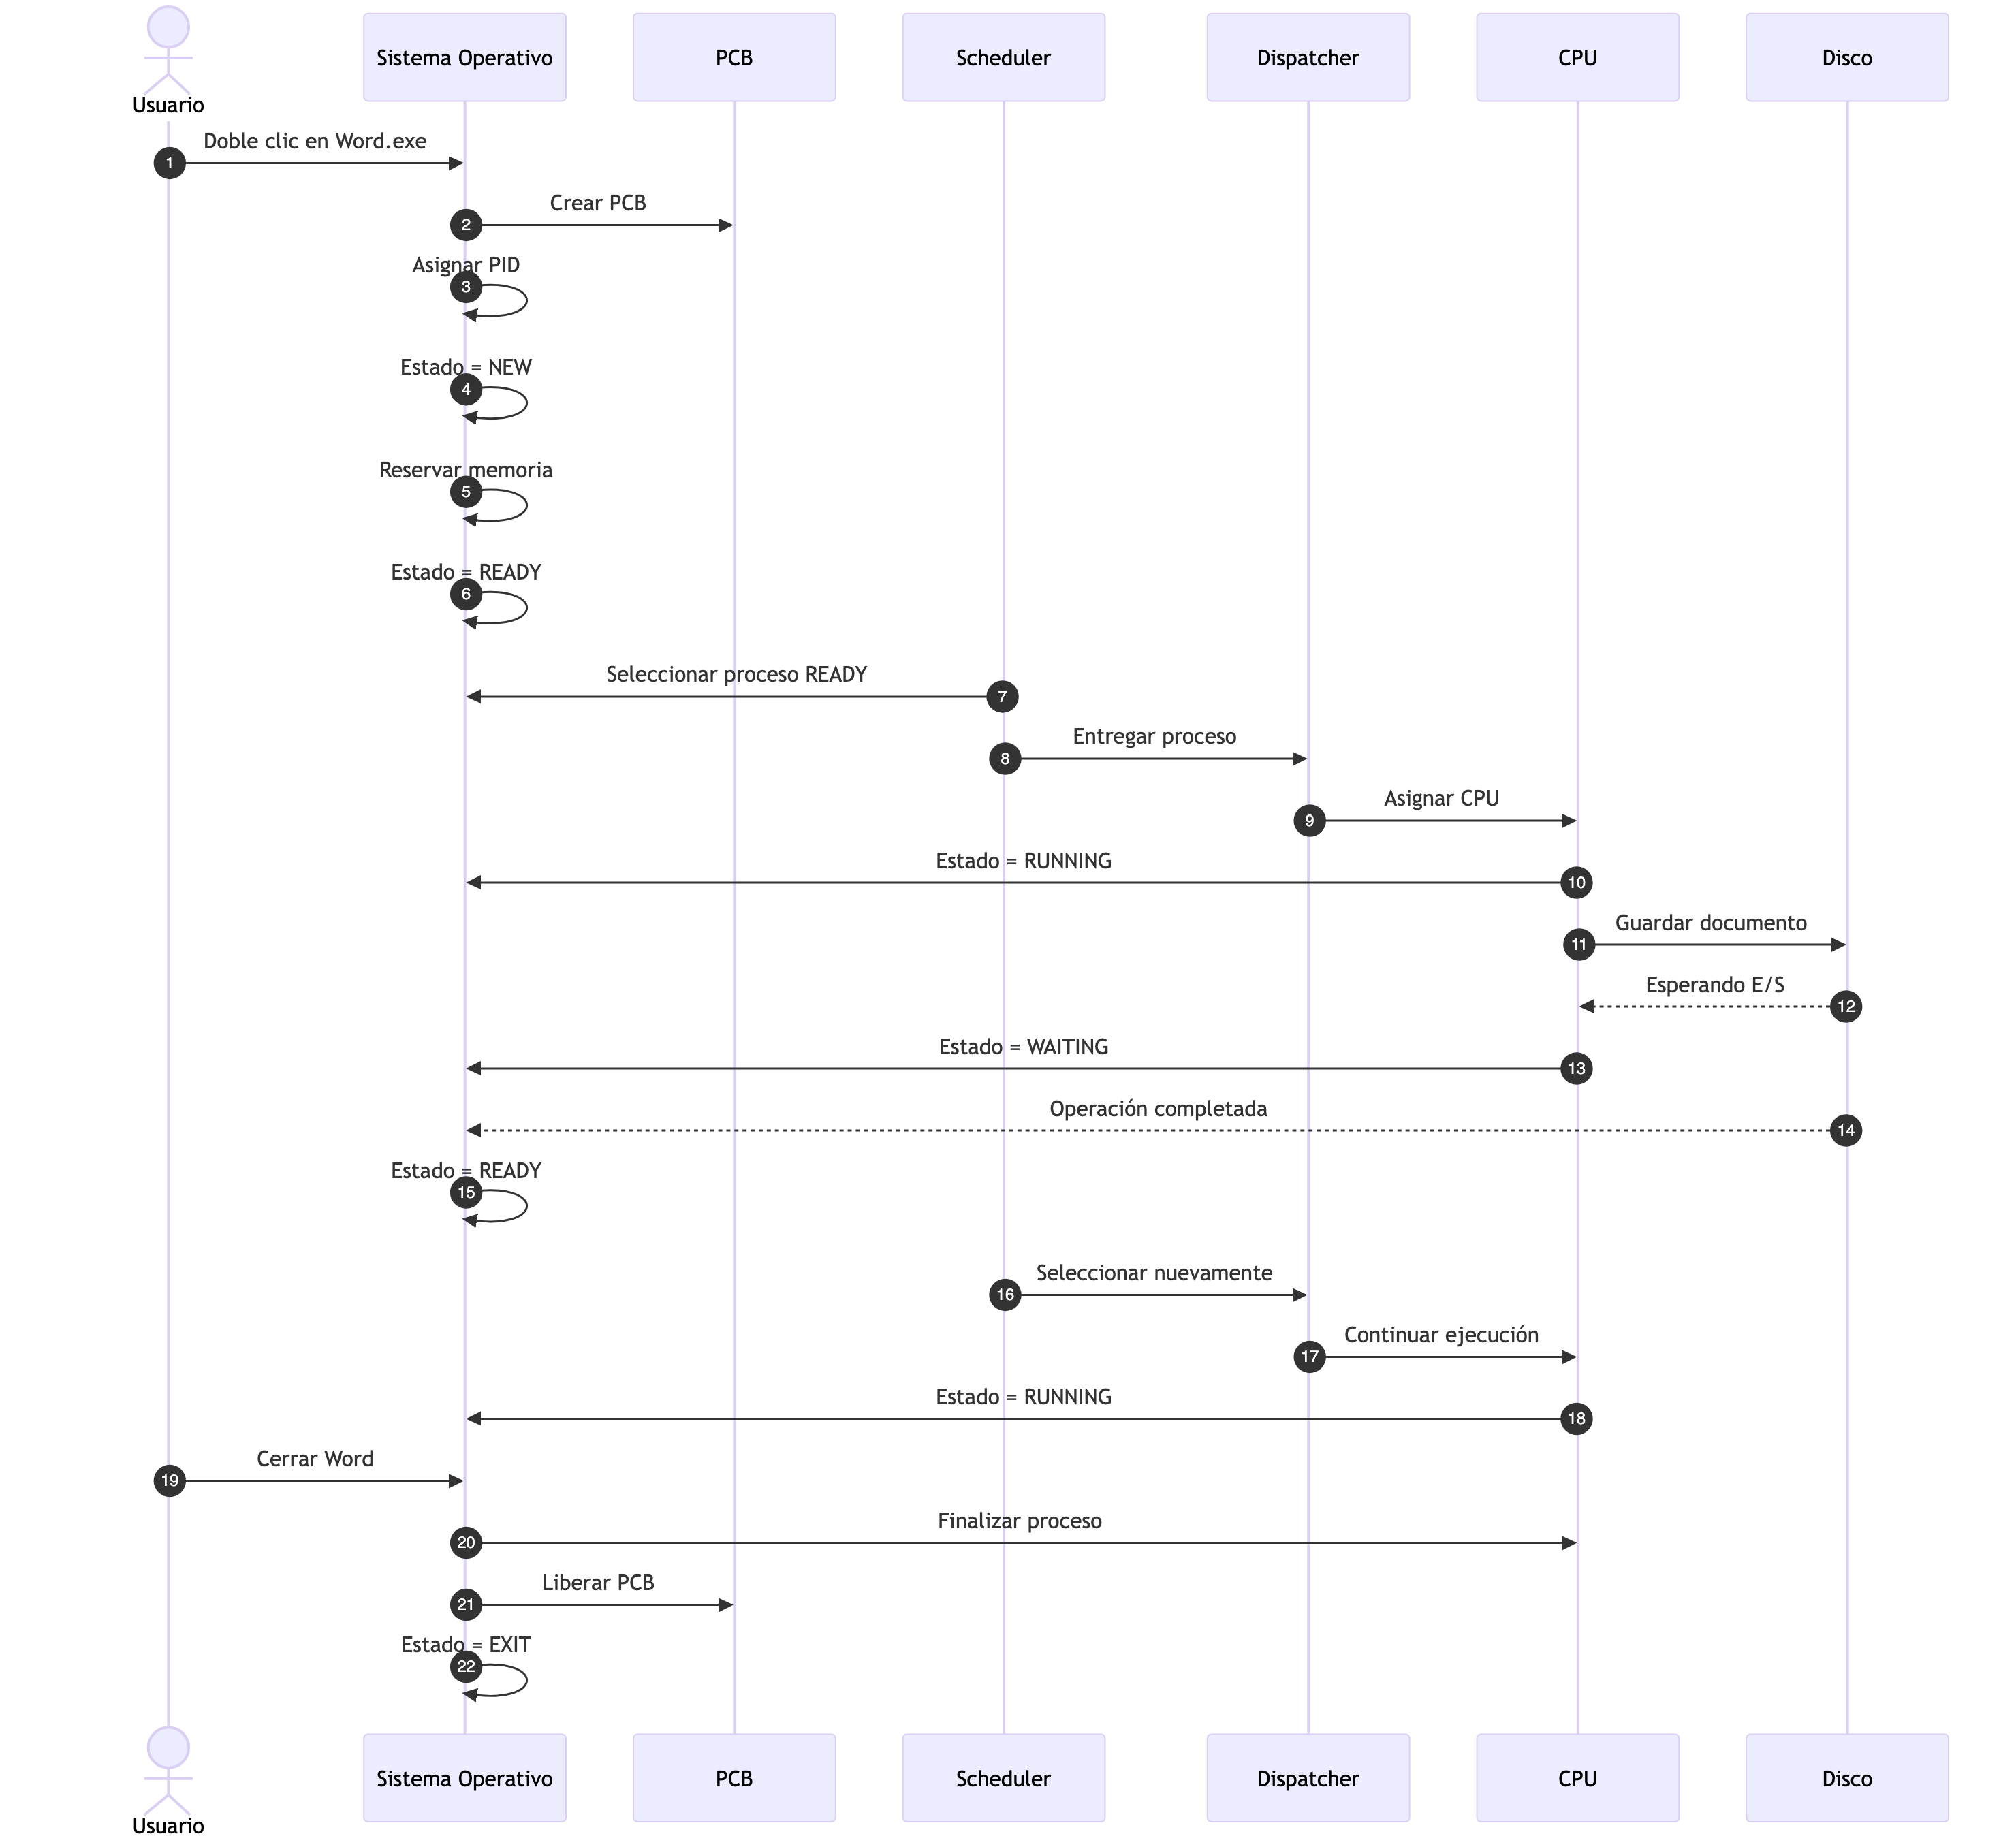
\includegraphics[width=6.2in,height=8.4in]{capitulos/04_administracion_procesos_files/figure-latex/mermaid-figure-2.png}

\section{Autoevaluación}\label{autoevaluaciuxf3n-1}

\begin{enumerate}
\def\labelenumi{\arabic{enumi}.}
\tightlist
\item
  ¿Cuál es la diferencia entre un programa y un proceso?
\item
  ¿Qué información almacena el PCB?
\item
  ¿Qué función cumple el Scheduler?
\item
  ¿Cuándo ocurre un cambio de contexto?
\item
  Explique el recorrido NEW → READY → RUNNING → WAITING → READY → EXIT
  con sus propias palabras.
\end{enumerate}

\bookmarksetup{startatroot}

\chapter{Cierre de la clase}\label{cierre-de-la-clase-1}

\begin{tcolorbox}[enhanced jigsaw, arc=.35mm, bottomrule=.15mm, bottomtitle=1mm, breakable, colback=white, colbacktitle=quarto-callout-tip-color!10!white, colframe=quarto-callout-tip-color-frame, coltitle=black, left=2mm, leftrule=.75mm, opacityback=0, opacitybacktitle=0.6, rightrule=.15mm, title=\textcolor{quarto-callout-tip-color}{\faLightbulb}\hspace{0.5em}{Consejo final del Ingeniero}, titlerule=0mm, toprule=.15mm, toptitle=1mm]

Comprender un sistema operativo no consiste solamente en aprender
nombres de versiones o comandos. Consiste en comprender cómo se
administran recursos, cómo se protegen los procesos y cómo se construye
el entorno donde funcionan las aplicaciones.

\end{tcolorbox}

\section{Próximo paso}\label{pruxf3ximo-paso}

En la siguiente clase profundizaremos en la estructura y los componentes
de un sistema operativo, relacionando kernel, procesos, memoria,
dispositivos y servicios.


\backmatter


\end{document}
